\documentclass[11pt,english,a4paper]{article}
\usepackage{babel}
\input{/home/marius/Dokumenter/preamples/phys_en.pre}
\author{\normalsize Marius Jonsson (Institutt for Vanskelig Fysikk, Oscars gate 19, 0352 OSLO, Norway) \\\\
\vspace{5px}
\normalsize \texttt{http://github.com/kingoslo/attaboy}}
\title{\bf \uppercase{TiTlE}}
\date{\normalsize \today}
\addbibresource{/home/marius/Dokumenter/MyLibrary.bib}
\DeclareUnicodeCharacter{2212}{$-$}
\begin{document}
\maketitle
\begin{abstract} \normalsize This is a report submission for the fourth project of «Computational physics» at the Institute of Physics, University of Oslo, autumn 2016.
\end{abstract}
\lstset{
  xleftmargin=.2\textwidth, xrightmargin=.2\textwidth
}



\section*{\uppercase{Introduction}}
> I Motivate the reader, the first part of the introduction gives always a motivation and tries to give the overarching ideas\\
> I What I have done\\
> I The structure of the report, how it is organized etc
\section*{\uppercase{Methods}}
We used the Metropolis algorithm in conjunction with the Ising model to approximate the Boltzman distribution $P(E)$. The Metropolis algorithm works by constructing a Markov chain such that the stationary distribution is $P$ (Robert, Christian; Casella, George (2004). Monte Carlo Statistical Methods). We know that a Markov chain is defined by its transition distribution. We know that detailed balance(hva) and ergodicity(hva) are sufficient but (but not required conditions) for existance and uniqueness of stationary distribution respectively.

Let's design a markov chain such that its stationary distripution is $P$. We will call this markov chain the Metropolis algorithm. We use the detailed balance criterion using P as the asymptotic distribution. This ensures that  the resulting markov chain will have P as an asymptotic distribution.
\[
p(i,j)P(j) = p(j,i)P(i) \qquad \text{only if} \qquad \frac{P(i)}{P(j)} = \frac{p(i,j)}{p(j,i)}
\]
Now pick any conditional distribution $g:\mathbb{R}^2 \to \mathbb{R}$ and a function $A: \mathbb{R}^2 \to \mathbb{R}$ such that
\begin{equation}
p(i,j) = g(i,j)A(i,j) \qquad \text{only if} \qquad \frac{A(i,j)}{A(j,i)} = \frac{P(i)}{P(j)} \frac{g(j,i)}{g(i,j)} \label{eq:mcchain}
\end{equation}
Clearly, by fixing the transformation rules of $A$ and $g$ one uniquely defines $p$ since $p$ is the pointwise product of $A$ with $g$. Let $g$ be any function on $\mathbb{R}^2$ with non-compact support, and define $A$ by
\begin{equation}
A(i,j) = \min \left( 1, \frac{P(i)}{P(j)} \frac{g(j,i)}{g(i,j)} \right),
\end{equation}
which solves equation \eqref{eq:mcchain} (check yourself!). This is the selection rule for the Metropolis algorithm as you will find implemented in this project.\\
\\
And sinec this markov chain is ergodic (Hjorth jensen), $P$ is the only stationary distribution of of $p$ (Robert, Christian; Casella, George (2004). Monte Carlo Statistical Methods). Let us consider how this is implemented in the case of the Ising model, where $A(i,j)/A(j,i)$ is taken to be the Boltzman factor.\\
\\
In this project we assume we are working with a sequence of $L \times L$ matrices $M_n$ where the elements $m_{u,v}$ are either $1$ or $-1$. Let $J$ be some real number, we assign a quantity called the energy denoted by $E$ which is computed by
\begin{equation}
E_n = -J \sum_{(i,j) \in S_L^2} (m_{ij} m_{i(j+1 \ \mathrm{mod} \ L)} + m_{ij} m_{(i+1 \ \mathrm{mod} \ L)j}), \label{energy}
\end{equation}
letting $S_L^2 = \big\{ (u,v) \in \{1,\cdots, L \}\times\{1,\cdots, L \} \big\}$, this ensures the sum in \eqref{energy} is over neighbouring elements of the matrix $M$ with periodic boundary conditions. We take the target distribution $P$ for the Metropolis algorithm to be the Boltzmann distribution. Hence $P(i) = (1/Z) e^{ -\beta E_i}$, for $\beta = (k_B T)^{  -1}$ and $k_B$ the Boltzmann constant. We let $g(i,j)$ be the unknown function induced by by the selection rule $A$ and Boltzmann factor when we flip one spin at a time. Bla bla\\
\\
The algorithm was implemented in c++ by:
\begin{lstlisting}[language=c++]
for (int k = 0; k < N; k++) { // sample iterations
    for (int i = 0; i < m; i++) { // loop matrix cols  
        for (int j = 0; j < n; j++) { // matrix rows
            int u = rand_int(gen);
            int v = rand_int(gen);
            double dE = 2*A[u][v]*(A[u][mod(v+1,n)] + 
                                       A[mod(u+1,m)][v] +
                                       A[u][mod(v-1,n)] + 
                                       A[mod(u-1,m)][v]);
            if (exp(-beta*dE) > rand_double(gen)) {
                // selection criterion                
                A[u][v] = - A[u][v];
                E += dE; 
                M += 2*A[u][v];
            }
        }
    }
    // sample if we believe we're at equilibrium
    if (k > samplepoint) {
        avg[0] += E;
        avg[1] += E*E;
        avg[2] += abs(M);
        avg[3] += M*M;
    }
}
\end{lstlisting}
We computed the exact result for $L=2$ and compared them to the numerical results. The errors were reasonable, indicating that the algorithm was implemented correctly (see table \ref{tab:errors}). The expressions for the exact results will be presented in the results.\\
\\
We would like to know when we have reached the asymptotic distribution $P$. Since we want to compute observables, this is useful because this ensures  that we know we are sampling to our expectation values from the Boltzmann distribution at any given confidence level. To test this, we will use a conventional $\chi^2$ statistical goodness-of-fit-test for the null hypothesis $H_0:$ $P(i)$ is the asymptotic distribution against $H_a:$ $P(i)$ is not the asymptotic distribution. The first markov iteration for which this is the case should be taken as the sampling point, because then we know that we are sampling from the Boltzmann distribution. We test this by at each step $n$ by assembling the asymptotic distribution by bootstrapping (Berk Devoire) and drawing samples from the empirical distribution at step $n$. We gather data by simulating $N$ times using the Metropolis algorithm. We let the algorithm continue for a long time, typically $10^6$ or $10^7$ Montecarlo cycles. We do this to ensure that the asnymptotic distribution is the Boltzman distribution. We store the measured energies at each monte carlo cycle $n$ for all the $N$ simulations. This means we have typically $10^6$ or $10^7$ candidates to the asymptotic distribution (the boltzmanm distribution). Since we did exactly $N$ simulations, we have $N$ observation from the candidates to the asymptotic distribution at each $n$. Each of these candidates are compared to asymptotic distribution. There exist statistical tests which can be used to determine when the sample is drawn from the asymptotic distribution for each $n$ at any confidence level $\alpha$. The most common is the chi-square goodness-of-fit test, which works as follows: At each $n$, divide cut the domain of the empirical distribution into $k$ intervals $I_j$ such that there are at least 5 observations in $I_j$ for all $j$. Count the number of observation in each interval, and label it by $n_j$. Then compute the probability of an observation to fall into $I_j$ from the empirical distribution. Call this probability $p_j$. It can be shown using the center limit theorem of dependent stochastic that the following observable has a known distribution:
\[
X^2 = \sum_{j=1}^k \frac{(n_j - np_j )^2}{np_j}.
\]
The distribution is the $\chi^2_\nu$-distribution with $\nu$ degrees of freedom, where $\nu = k-1$ under the null hypothesis that the empirical distribution is equal to the empirical. In the case that the null-hypothesis is false, the value of $X^2$ will be large, and when the value of $X^2$ is larger than the $\chi^2_{\nu, 1-\alpha}$-quantile in the $\chi^2$-distribution, we know that the distributions are difference at confidence level $\alpha$. We chose a confidence level of $0.5$, which implies we will only accept distributions which are so similar to the asymptotic distribution, that the probability of evaluating a distribution violating the null more hypothesis more strongly is exactly 50\%.
\section*{\uppercase{Results and discussion}}
\begin{table}[!h]
\center
\begin{tabular}{c l l l}
Observable&Exact:					& Numerical, $n = 10^8$& Error\\
\hline
$\E{E}$ & -7.9839283437467596		& -7.98379632& $-1.3\cdot 10^{-4}$\\
$\E{|M|}$ & 3.9946429309943987		& 3.9945928& $5.0\cdot 10^{-5}$\\
$C_V$ & 0.12832932745714487	& 0.129378400754& $-1.0\cdot 10^{-3}$\\
$\chi$ & 0.01604295806490974		& 0.0162110021882& $-1.7\cdot 10^{-4}$
\end{tabular}
\caption{BLa bla} \label{tab:errors}
\end{table}

\begin{figure}
\center
% Created by tikzDevice version 0.10.1 on 2016-11-13 23:03:50
% !TEX encoding = UTF-8 Unicode
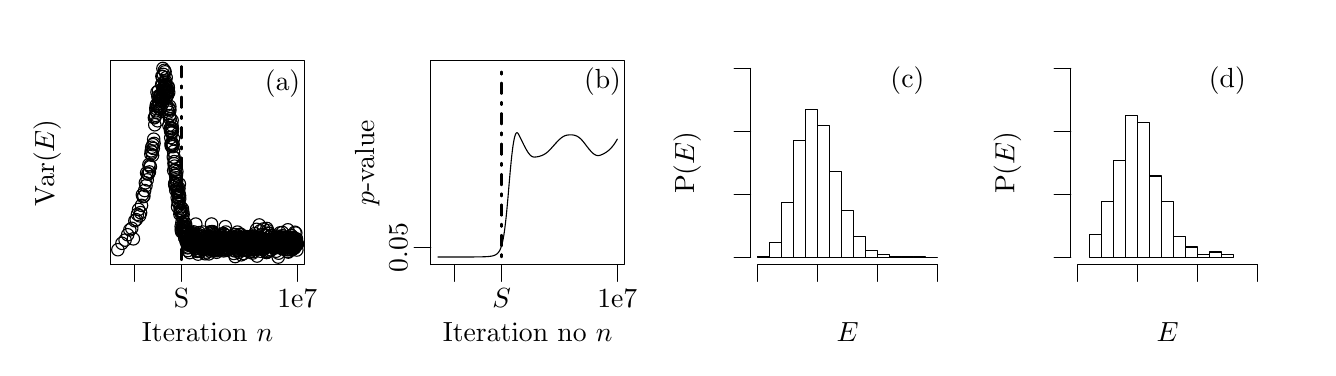
\begin{tikzpicture}[x=1pt,y=1pt]
\definecolor{fillColor}{RGB}{255,255,255}
\path[use as bounding box,fill=fillColor,fill opacity=0.00] (0,0) rectangle (462.53,115.63);
\begin{scope}
\path[clip] ( 30.00, 30.00) rectangle (100.03,103.63);
\definecolor{drawColor}{RGB}{0,0,0}

\path[draw=drawColor,line width= 0.4pt,line join=round,line cap=round] ( 32.59, 35.39) circle (  2.25);

\path[draw=drawColor,line width= 0.4pt,line join=round,line cap=round] ( 34.06, 37.71) circle (  2.25);

\path[draw=drawColor,line width= 0.4pt,line join=round,line cap=round] ( 35.20, 38.87) circle (  2.25);

\path[draw=drawColor,line width= 0.4pt,line join=round,line cap=round] ( 36.13, 40.80) circle (  2.25);

\path[draw=drawColor,line width= 0.4pt,line join=round,line cap=round] ( 36.91, 42.55) circle (  2.25);

\path[draw=drawColor,line width= 0.4pt,line join=round,line cap=round] ( 37.60, 43.13) circle (  2.25);

\path[draw=drawColor,line width= 0.4pt,line join=round,line cap=round] ( 38.20, 39.32) circle (  2.25);

\path[draw=drawColor,line width= 0.4pt,line join=round,line cap=round] ( 38.73, 45.85) circle (  2.25);

\path[draw=drawColor,line width= 0.4pt,line join=round,line cap=round] ( 39.22, 46.25) circle (  2.25);

\path[draw=drawColor,line width= 0.4pt,line join=round,line cap=round] ( 39.66, 48.18) circle (  2.25);

\path[draw=drawColor,line width= 0.4pt,line join=round,line cap=round] ( 40.07, 49.94) circle (  2.25);

\path[draw=drawColor,line width= 0.4pt,line join=round,line cap=round] ( 40.45, 47.65) circle (  2.25);

\path[draw=drawColor,line width= 0.4pt,line join=round,line cap=round] ( 40.80, 48.79) circle (  2.25);

\path[draw=drawColor,line width= 0.4pt,line join=round,line cap=round] ( 41.13, 51.42) circle (  2.25);

\path[draw=drawColor,line width= 0.4pt,line join=round,line cap=round] ( 41.44, 55.24) circle (  2.25);

\path[draw=drawColor,line width= 0.4pt,line join=round,line cap=round] ( 41.73, 54.56) circle (  2.25);

\path[draw=drawColor,line width= 0.4pt,line join=round,line cap=round] ( 42.01, 54.80) circle (  2.25);

\path[draw=drawColor,line width= 0.4pt,line join=round,line cap=round] ( 42.27, 56.78) circle (  2.25);

\path[draw=drawColor,line width= 0.4pt,line join=round,line cap=round] ( 42.52, 59.58) circle (  2.25);

\path[draw=drawColor,line width= 0.4pt,line join=round,line cap=round] ( 42.75, 58.52) circle (  2.25);

\path[draw=drawColor,line width= 0.4pt,line join=round,line cap=round] ( 42.98, 63.16) circle (  2.25);

\path[draw=drawColor,line width= 0.4pt,line join=round,line cap=round] ( 43.20, 60.63) circle (  2.25);

\path[draw=drawColor,line width= 0.4pt,line join=round,line cap=round] ( 43.41, 62.76) circle (  2.25);

\path[draw=drawColor,line width= 0.4pt,line join=round,line cap=round] ( 43.61, 62.76) circle (  2.25);

\path[draw=drawColor,line width= 0.4pt,line join=round,line cap=round] ( 43.80, 66.14) circle (  2.25);

\path[draw=drawColor,line width= 0.4pt,line join=round,line cap=round] ( 43.98, 63.49) circle (  2.25);

\path[draw=drawColor,line width= 0.4pt,line join=round,line cap=round] ( 44.16, 65.70) circle (  2.25);

\path[draw=drawColor,line width= 0.4pt,line join=round,line cap=round] ( 44.33, 65.35) circle (  2.25);

\path[draw=drawColor,line width= 0.4pt,line join=round,line cap=round] ( 44.50, 69.93) circle (  2.25);

\path[draw=drawColor,line width= 0.4pt,line join=round,line cap=round] ( 44.66, 71.13) circle (  2.25);

\path[draw=drawColor,line width= 0.4pt,line join=round,line cap=round] ( 44.82, 72.42) circle (  2.25);

\path[draw=drawColor,line width= 0.4pt,line join=round,line cap=round] ( 44.97, 70.68) circle (  2.25);

\path[draw=drawColor,line width= 0.4pt,line join=round,line cap=round] ( 45.12, 69.47) circle (  2.25);

\path[draw=drawColor,line width= 0.4pt,line join=round,line cap=round] ( 45.26, 73.35) circle (  2.25);

\path[draw=drawColor,line width= 0.4pt,line join=round,line cap=round] ( 45.40, 72.00) circle (  2.25);

\path[draw=drawColor,line width= 0.4pt,line join=round,line cap=round] ( 45.54, 75.33) circle (  2.25);

\path[draw=drawColor,line width= 0.4pt,line join=round,line cap=round] ( 45.67, 73.80) circle (  2.25);

\path[draw=drawColor,line width= 0.4pt,line join=round,line cap=round] ( 45.80, 83.07) circle (  2.25);

\path[draw=drawColor,line width= 0.4pt,line join=round,line cap=round] ( 45.93, 80.54) circle (  2.25);

\path[draw=drawColor,line width= 0.4pt,line join=round,line cap=round] ( 46.05, 83.40) circle (  2.25);

\path[draw=drawColor,line width= 0.4pt,line join=round,line cap=round] ( 46.17, 83.94) circle (  2.25);

\path[draw=drawColor,line width= 0.4pt,line join=round,line cap=round] ( 46.29, 86.46) circle (  2.25);

\path[draw=drawColor,line width= 0.4pt,line join=round,line cap=round] ( 46.40, 85.60) circle (  2.25);

\path[draw=drawColor,line width= 0.4pt,line join=round,line cap=round] ( 46.51, 87.72) circle (  2.25);

\path[draw=drawColor,line width= 0.4pt,line join=round,line cap=round] ( 46.62, 85.08) circle (  2.25);

\path[draw=drawColor,line width= 0.4pt,line join=round,line cap=round] ( 46.73, 92.33) circle (  2.25);

\path[draw=drawColor,line width= 0.4pt,line join=round,line cap=round] ( 46.84, 87.23) circle (  2.25);

\path[draw=drawColor,line width= 0.4pt,line join=round,line cap=round] ( 46.94, 81.99) circle (  2.25);

\path[draw=drawColor,line width= 0.4pt,line join=round,line cap=round] ( 47.04, 90.74) circle (  2.25);

\path[draw=drawColor,line width= 0.4pt,line join=round,line cap=round] ( 47.14, 87.29) circle (  2.25);

\path[draw=drawColor,line width= 0.4pt,line join=round,line cap=round] ( 47.24, 92.75) circle (  2.25);

\path[draw=drawColor,line width= 0.4pt,line join=round,line cap=round] ( 47.33, 88.89) circle (  2.25);

\path[draw=drawColor,line width= 0.4pt,line join=round,line cap=round] ( 47.43, 90.53) circle (  2.25);

\path[draw=drawColor,line width= 0.4pt,line join=round,line cap=round] ( 47.52, 87.33) circle (  2.25);

\path[draw=drawColor,line width= 0.4pt,line join=round,line cap=round] ( 47.61, 88.27) circle (  2.25);

\path[draw=drawColor,line width= 0.4pt,line join=round,line cap=round] ( 47.70, 90.42) circle (  2.25);

\path[draw=drawColor,line width= 0.4pt,line join=round,line cap=round] ( 47.78, 86.25) circle (  2.25);

\path[draw=drawColor,line width= 0.4pt,line join=round,line cap=round] ( 47.87, 86.13) circle (  2.25);

\path[draw=drawColor,line width= 0.4pt,line join=round,line cap=round] ( 47.95, 89.48) circle (  2.25);

\path[draw=drawColor,line width= 0.4pt,line join=round,line cap=round] ( 48.04, 91.50) circle (  2.25);

\path[draw=drawColor,line width= 0.4pt,line join=round,line cap=round] ( 48.12, 86.83) circle (  2.25);

\path[draw=drawColor,line width= 0.4pt,line join=round,line cap=round] ( 48.20, 89.86) circle (  2.25);

\path[draw=drawColor,line width= 0.4pt,line join=round,line cap=round] ( 48.28, 90.21) circle (  2.25);

\path[draw=drawColor,line width= 0.4pt,line join=round,line cap=round] ( 48.36, 90.54) circle (  2.25);

\path[draw=drawColor,line width= 0.4pt,line join=round,line cap=round] ( 48.43, 95.19) circle (  2.25);

\path[draw=drawColor,line width= 0.4pt,line join=round,line cap=round] ( 48.51, 98.07) circle (  2.25);

\path[draw=drawColor,line width= 0.4pt,line join=round,line cap=round] ( 48.58, 94.76) circle (  2.25);

\path[draw=drawColor,line width= 0.4pt,line join=round,line cap=round] ( 48.66, 88.14) circle (  2.25);

\path[draw=drawColor,line width= 0.4pt,line join=round,line cap=round] ( 48.73, 90.07) circle (  2.25);

\path[draw=drawColor,line width= 0.4pt,line join=round,line cap=round] ( 48.80, 97.91) circle (  2.25);

\path[draw=drawColor,line width= 0.4pt,line join=round,line cap=round] ( 48.87,100.90) circle (  2.25);

\path[draw=drawColor,line width= 0.4pt,line join=round,line cap=round] ( 48.94, 93.91) circle (  2.25);

\path[draw=drawColor,line width= 0.4pt,line join=round,line cap=round] ( 49.01, 98.75) circle (  2.25);

\path[draw=drawColor,line width= 0.4pt,line join=round,line cap=round] ( 49.07, 91.74) circle (  2.25);

\path[draw=drawColor,line width= 0.4pt,line join=round,line cap=round] ( 49.14, 90.18) circle (  2.25);

\path[draw=drawColor,line width= 0.4pt,line join=round,line cap=round] ( 49.21, 94.12) circle (  2.25);

\path[draw=drawColor,line width= 0.4pt,line join=round,line cap=round] ( 49.27, 92.99) circle (  2.25);

\path[draw=drawColor,line width= 0.4pt,line join=round,line cap=round] ( 49.34, 92.24) circle (  2.25);

\path[draw=drawColor,line width= 0.4pt,line join=round,line cap=round] ( 49.40,100.22) circle (  2.25);

\path[draw=drawColor,line width= 0.4pt,line join=round,line cap=round] ( 49.46, 93.83) circle (  2.25);

\path[draw=drawColor,line width= 0.4pt,line join=round,line cap=round] ( 49.52, 95.98) circle (  2.25);

\path[draw=drawColor,line width= 0.4pt,line join=round,line cap=round] ( 49.58, 92.80) circle (  2.25);

\path[draw=drawColor,line width= 0.4pt,line join=round,line cap=round] ( 49.65, 99.67) circle (  2.25);

\path[draw=drawColor,line width= 0.4pt,line join=round,line cap=round] ( 49.70, 95.09) circle (  2.25);

\path[draw=drawColor,line width= 0.4pt,line join=round,line cap=round] ( 49.82, 96.36) circle (  2.25);

\path[draw=drawColor,line width= 0.4pt,line join=round,line cap=round] ( 49.88, 94.43) circle (  2.25);

\path[draw=drawColor,line width= 0.4pt,line join=round,line cap=round] ( 49.94, 94.87) circle (  2.25);

\path[draw=drawColor,line width= 0.4pt,line join=round,line cap=round] ( 49.99, 94.18) circle (  2.25);

\path[draw=drawColor,line width= 0.4pt,line join=round,line cap=round] ( 50.05, 97.59) circle (  2.25);

\path[draw=drawColor,line width= 0.4pt,line join=round,line cap=round] ( 50.10, 90.54) circle (  2.25);

\path[draw=drawColor,line width= 0.4pt,line join=round,line cap=round] ( 50.21, 87.62) circle (  2.25);

\path[draw=drawColor,line width= 0.4pt,line join=round,line cap=round] ( 50.27, 92.31) circle (  2.25);

\path[draw=drawColor,line width= 0.4pt,line join=round,line cap=round] ( 50.32, 91.09) circle (  2.25);

\path[draw=drawColor,line width= 0.4pt,line join=round,line cap=round] ( 50.37, 92.15) circle (  2.25);

\path[draw=drawColor,line width= 0.4pt,line join=round,line cap=round] ( 50.42, 92.64) circle (  2.25);

\path[draw=drawColor,line width= 0.4pt,line join=round,line cap=round] ( 50.52, 85.96) circle (  2.25);

\path[draw=drawColor,line width= 0.4pt,line join=round,line cap=round] ( 50.57, 91.36) circle (  2.25);

\path[draw=drawColor,line width= 0.4pt,line join=round,line cap=round] ( 50.62, 92.43) circle (  2.25);

\path[draw=drawColor,line width= 0.4pt,line join=round,line cap=round] ( 50.72, 93.11) circle (  2.25);

\path[draw=drawColor,line width= 0.4pt,line join=round,line cap=round] ( 50.77, 94.33) circle (  2.25);

\path[draw=drawColor,line width= 0.4pt,line join=round,line cap=round] ( 50.82, 93.88) circle (  2.25);

\path[draw=drawColor,line width= 0.4pt,line join=round,line cap=round] ( 50.91, 85.11) circle (  2.25);

\path[draw=drawColor,line width= 0.4pt,line join=round,line cap=round] ( 50.96, 92.22) circle (  2.25);

\path[draw=drawColor,line width= 0.4pt,line join=round,line cap=round] ( 51.05, 80.28) circle (  2.25);

\path[draw=drawColor,line width= 0.4pt,line join=round,line cap=round] ( 51.10, 86.20) circle (  2.25);

\path[draw=drawColor,line width= 0.4pt,line join=round,line cap=round] ( 51.14, 86.38) circle (  2.25);

\path[draw=drawColor,line width= 0.4pt,line join=round,line cap=round] ( 51.23, 83.78) circle (  2.25);

\path[draw=drawColor,line width= 0.4pt,line join=round,line cap=round] ( 51.27, 83.88) circle (  2.25);

\path[draw=drawColor,line width= 0.4pt,line join=round,line cap=round] ( 51.36, 87.19) circle (  2.25);

\path[draw=drawColor,line width= 0.4pt,line join=round,line cap=round] ( 51.40, 85.85) circle (  2.25);

\path[draw=drawColor,line width= 0.4pt,line join=round,line cap=round] ( 51.49, 82.62) circle (  2.25);

\path[draw=drawColor,line width= 0.4pt,line join=round,line cap=round] ( 51.57, 79.39) circle (  2.25);

\path[draw=drawColor,line width= 0.4pt,line join=round,line cap=round] ( 51.61, 78.37) circle (  2.25);

\path[draw=drawColor,line width= 0.4pt,line join=round,line cap=round] ( 51.69, 75.88) circle (  2.25);

\path[draw=drawColor,line width= 0.4pt,line join=round,line cap=round] ( 51.73, 78.59) circle (  2.25);

\path[draw=drawColor,line width= 0.4pt,line join=round,line cap=round] ( 51.81, 73.45) circle (  2.25);

\path[draw=drawColor,line width= 0.4pt,line join=round,line cap=round] ( 51.89, 72.83) circle (  2.25);

\path[draw=drawColor,line width= 0.4pt,line join=round,line cap=round] ( 51.93, 73.92) circle (  2.25);

\path[draw=drawColor,line width= 0.4pt,line join=round,line cap=round] ( 52.00, 77.52) circle (  2.25);

\path[draw=drawColor,line width= 0.4pt,line join=round,line cap=round] ( 52.08, 79.27) circle (  2.25);

\path[draw=drawColor,line width= 0.4pt,line join=round,line cap=round] ( 52.15, 80.37) circle (  2.25);

\path[draw=drawColor,line width= 0.4pt,line join=round,line cap=round] ( 52.19, 82.12) circle (  2.25);

\path[draw=drawColor,line width= 0.4pt,line join=round,line cap=round] ( 52.26, 78.12) circle (  2.25);

\path[draw=drawColor,line width= 0.4pt,line join=round,line cap=round] ( 52.33, 79.06) circle (  2.25);

\path[draw=drawColor,line width= 0.4pt,line join=round,line cap=round] ( 52.40, 72.61) circle (  2.25);

\path[draw=drawColor,line width= 0.4pt,line join=round,line cap=round] ( 52.47, 73.56) circle (  2.25);

\path[draw=drawColor,line width= 0.4pt,line join=round,line cap=round] ( 52.54, 73.38) circle (  2.25);

\path[draw=drawColor,line width= 0.4pt,line join=round,line cap=round] ( 52.61, 68.87) circle (  2.25);

\path[draw=drawColor,line width= 0.4pt,line join=round,line cap=round] ( 52.68, 75.51) circle (  2.25);

\path[draw=drawColor,line width= 0.4pt,line join=round,line cap=round] ( 52.71, 70.89) circle (  2.25);

\path[draw=drawColor,line width= 0.4pt,line join=round,line cap=round] ( 52.77, 64.01) circle (  2.25);

\path[draw=drawColor,line width= 0.4pt,line join=round,line cap=round] ( 52.87, 66.49) circle (  2.25);

\path[draw=drawColor,line width= 0.4pt,line join=round,line cap=round] ( 52.93, 68.72) circle (  2.25);

\path[draw=drawColor,line width= 0.4pt,line join=round,line cap=round] ( 53.00, 67.23) circle (  2.25);

\path[draw=drawColor,line width= 0.4pt,line join=round,line cap=round] ( 53.06, 65.61) circle (  2.25);

\path[draw=drawColor,line width= 0.4pt,line join=round,line cap=round] ( 53.12, 59.12) circle (  2.25);

\path[draw=drawColor,line width= 0.4pt,line join=round,line cap=round] ( 53.18, 59.38) circle (  2.25);

\path[draw=drawColor,line width= 0.4pt,line join=round,line cap=round] ( 53.24, 58.54) circle (  2.25);

\path[draw=drawColor,line width= 0.4pt,line join=round,line cap=round] ( 53.30, 64.22) circle (  2.25);

\path[draw=drawColor,line width= 0.4pt,line join=round,line cap=round] ( 53.39, 64.17) circle (  2.25);

\path[draw=drawColor,line width= 0.4pt,line join=round,line cap=round] ( 53.44, 62.31) circle (  2.25);

\path[draw=drawColor,line width= 0.4pt,line join=round,line cap=round] ( 53.50, 56.91) circle (  2.25);

\path[draw=drawColor,line width= 0.4pt,line join=round,line cap=round] ( 53.58, 60.65) circle (  2.25);

\path[draw=drawColor,line width= 0.4pt,line join=round,line cap=round] ( 53.64, 61.36) circle (  2.25);

\path[draw=drawColor,line width= 0.4pt,line join=round,line cap=round] ( 53.69, 58.90) circle (  2.25);

\path[draw=drawColor,line width= 0.4pt,line join=round,line cap=round] ( 53.77, 62.42) circle (  2.25);

\path[draw=drawColor,line width= 0.4pt,line join=round,line cap=round] ( 53.83, 60.17) circle (  2.25);

\path[draw=drawColor,line width= 0.4pt,line join=round,line cap=round] ( 53.91, 63.63) circle (  2.25);

\path[draw=drawColor,line width= 0.4pt,line join=round,line cap=round] ( 53.96, 57.38) circle (  2.25);

\path[draw=drawColor,line width= 0.4pt,line join=round,line cap=round] ( 54.03, 54.17) circle (  2.25);

\path[draw=drawColor,line width= 0.4pt,line join=round,line cap=round] ( 54.08, 56.07) circle (  2.25);

\path[draw=drawColor,line width= 0.4pt,line join=round,line cap=round] ( 54.16, 50.88) circle (  2.25);

\path[draw=drawColor,line width= 0.4pt,line join=round,line cap=round] ( 54.23, 56.47) circle (  2.25);

\path[draw=drawColor,line width= 0.4pt,line join=round,line cap=round] ( 54.28, 57.47) circle (  2.25);

\path[draw=drawColor,line width= 0.4pt,line join=round,line cap=round] ( 54.35, 52.45) circle (  2.25);

\path[draw=drawColor,line width= 0.4pt,line join=round,line cap=round] ( 54.42, 56.55) circle (  2.25);

\path[draw=drawColor,line width= 0.4pt,line join=round,line cap=round] ( 54.49, 52.73) circle (  2.25);

\path[draw=drawColor,line width= 0.4pt,line join=round,line cap=round] ( 54.54, 54.34) circle (  2.25);

\path[draw=drawColor,line width= 0.4pt,line join=round,line cap=round] ( 54.61, 54.42) circle (  2.25);

\path[draw=drawColor,line width= 0.4pt,line join=round,line cap=round] ( 54.68, 57.60) circle (  2.25);

\path[draw=drawColor,line width= 0.4pt,line join=round,line cap=round] ( 54.74, 55.44) circle (  2.25);

\path[draw=drawColor,line width= 0.4pt,line join=round,line cap=round] ( 54.81, 59.17) circle (  2.25);

\path[draw=drawColor,line width= 0.4pt,line join=round,line cap=round] ( 54.87, 55.00) circle (  2.25);

\path[draw=drawColor,line width= 0.4pt,line join=round,line cap=round] ( 54.94, 53.83) circle (  2.25);

\path[draw=drawColor,line width= 0.4pt,line join=round,line cap=round] ( 55.00, 48.23) circle (  2.25);

\path[draw=drawColor,line width= 0.4pt,line join=round,line cap=round] ( 55.06, 50.39) circle (  2.25);

\path[draw=drawColor,line width= 0.4pt,line join=round,line cap=round] ( 55.15, 49.43) circle (  2.25);

\path[draw=drawColor,line width= 0.4pt,line join=round,line cap=round] ( 55.21, 48.93) circle (  2.25);

\path[draw=drawColor,line width= 0.4pt,line join=round,line cap=round] ( 55.27, 49.57) circle (  2.25);

\path[draw=drawColor,line width= 0.4pt,line join=round,line cap=round] ( 55.33, 50.88) circle (  2.25);

\path[draw=drawColor,line width= 0.4pt,line join=round,line cap=round] ( 55.40, 49.32) circle (  2.25);

\path[draw=drawColor,line width= 0.4pt,line join=round,line cap=round] ( 55.46, 43.80) circle (  2.25);

\path[draw=drawColor,line width= 0.4pt,line join=round,line cap=round] ( 55.52, 42.37) circle (  2.25);

\path[draw=drawColor,line width= 0.4pt,line join=round,line cap=round] ( 55.59, 42.75) circle (  2.25);

\path[draw=drawColor,line width= 0.4pt,line join=round,line cap=round] ( 55.65, 41.84) circle (  2.25);

\path[draw=drawColor,line width= 0.4pt,line join=round,line cap=round] ( 55.72, 45.14) circle (  2.25);

\path[draw=drawColor,line width= 0.4pt,line join=round,line cap=round] ( 55.80, 42.48) circle (  2.25);

\path[draw=drawColor,line width= 0.4pt,line join=round,line cap=round] ( 55.85, 47.24) circle (  2.25);

\path[draw=drawColor,line width= 0.4pt,line join=round,line cap=round] ( 55.92, 50.17) circle (  2.25);

\path[draw=drawColor,line width= 0.4pt,line join=round,line cap=round] ( 55.99, 43.75) circle (  2.25);

\path[draw=drawColor,line width= 0.4pt,line join=round,line cap=round] ( 56.04, 49.04) circle (  2.25);

\path[draw=drawColor,line width= 0.4pt,line join=round,line cap=round] ( 56.11, 43.96) circle (  2.25);

\path[draw=drawColor,line width= 0.4pt,line join=round,line cap=round] ( 56.18, 48.11) circle (  2.25);

\path[draw=drawColor,line width= 0.4pt,line join=round,line cap=round] ( 56.24, 42.08) circle (  2.25);

\path[draw=drawColor,line width= 0.4pt,line join=round,line cap=round] ( 56.31, 44.59) circle (  2.25);

\path[draw=drawColor,line width= 0.4pt,line join=round,line cap=round] ( 56.37, 43.39) circle (  2.25);

\path[draw=drawColor,line width= 0.4pt,line join=round,line cap=round] ( 56.44, 45.61) circle (  2.25);

\path[draw=drawColor,line width= 0.4pt,line join=round,line cap=round] ( 56.50, 42.92) circle (  2.25);

\path[draw=drawColor,line width= 0.4pt,line join=round,line cap=round] ( 56.58, 41.80) circle (  2.25);

\path[draw=drawColor,line width= 0.4pt,line join=round,line cap=round] ( 56.64, 41.00) circle (  2.25);

\path[draw=drawColor,line width= 0.4pt,line join=round,line cap=round] ( 56.70, 42.52) circle (  2.25);

\path[draw=drawColor,line width= 0.4pt,line join=round,line cap=round] ( 56.77, 39.70) circle (  2.25);

\path[draw=drawColor,line width= 0.4pt,line join=round,line cap=round] ( 56.83, 39.69) circle (  2.25);

\path[draw=drawColor,line width= 0.4pt,line join=round,line cap=round] ( 56.89, 42.86) circle (  2.25);

\path[draw=drawColor,line width= 0.4pt,line join=round,line cap=round] ( 56.96, 43.60) circle (  2.25);

\path[draw=drawColor,line width= 0.4pt,line join=round,line cap=round] ( 57.03, 43.74) circle (  2.25);

\path[draw=drawColor,line width= 0.4pt,line join=round,line cap=round] ( 57.09, 44.55) circle (  2.25);

\path[draw=drawColor,line width= 0.4pt,line join=round,line cap=round] ( 57.16, 41.54) circle (  2.25);

\path[draw=drawColor,line width= 0.4pt,line join=round,line cap=round] ( 57.23, 38.35) circle (  2.25);

\path[draw=drawColor,line width= 0.4pt,line join=round,line cap=round] ( 57.29, 39.88) circle (  2.25);

\path[draw=drawColor,line width= 0.4pt,line join=round,line cap=round] ( 57.35, 42.09) circle (  2.25);

\path[draw=drawColor,line width= 0.4pt,line join=round,line cap=round] ( 57.41, 40.99) circle (  2.25);

\path[draw=drawColor,line width= 0.4pt,line join=round,line cap=round] ( 57.48, 41.64) circle (  2.25);

\path[draw=drawColor,line width= 0.4pt,line join=round,line cap=round] ( 57.56, 37.61) circle (  2.25);

\path[draw=drawColor,line width= 0.4pt,line join=round,line cap=round] ( 57.62, 38.52) circle (  2.25);

\path[draw=drawColor,line width= 0.4pt,line join=round,line cap=round] ( 57.68, 40.49) circle (  2.25);

\path[draw=drawColor,line width= 0.4pt,line join=round,line cap=round] ( 57.74, 41.76) circle (  2.25);

\path[draw=drawColor,line width= 0.4pt,line join=round,line cap=round] ( 57.82, 36.07) circle (  2.25);

\path[draw=drawColor,line width= 0.4pt,line join=round,line cap=round] ( 57.88, 35.09) circle (  2.25);

\path[draw=drawColor,line width= 0.4pt,line join=round,line cap=round] ( 57.95, 36.36) circle (  2.25);

\path[draw=drawColor,line width= 0.4pt,line join=round,line cap=round] ( 58.01, 37.30) circle (  2.25);

\path[draw=drawColor,line width= 0.4pt,line join=round,line cap=round] ( 58.07, 37.03) circle (  2.25);

\path[draw=drawColor,line width= 0.4pt,line join=round,line cap=round] ( 58.13, 37.37) circle (  2.25);

\path[draw=drawColor,line width= 0.4pt,line join=round,line cap=round] ( 58.20, 40.39) circle (  2.25);

\path[draw=drawColor,line width= 0.4pt,line join=round,line cap=round] ( 58.27, 38.65) circle (  2.25);

\path[draw=drawColor,line width= 0.4pt,line join=round,line cap=round] ( 58.33, 39.08) circle (  2.25);

\path[draw=drawColor,line width= 0.4pt,line join=round,line cap=round] ( 58.40, 37.15) circle (  2.25);

\path[draw=drawColor,line width= 0.4pt,line join=round,line cap=round] ( 58.46, 37.56) circle (  2.25);

\path[draw=drawColor,line width= 0.4pt,line join=round,line cap=round] ( 58.53, 34.35) circle (  2.25);

\path[draw=drawColor,line width= 0.4pt,line join=round,line cap=round] ( 58.60, 38.75) circle (  2.25);

\path[draw=drawColor,line width= 0.4pt,line join=round,line cap=round] ( 58.66, 37.00) circle (  2.25);

\path[draw=drawColor,line width= 0.4pt,line join=round,line cap=round] ( 58.72, 38.70) circle (  2.25);

\path[draw=drawColor,line width= 0.4pt,line join=round,line cap=round] ( 58.79, 37.83) circle (  2.25);

\path[draw=drawColor,line width= 0.4pt,line join=round,line cap=round] ( 58.85, 40.87) circle (  2.25);

\path[draw=drawColor,line width= 0.4pt,line join=round,line cap=round] ( 58.92, 37.73) circle (  2.25);

\path[draw=drawColor,line width= 0.4pt,line join=round,line cap=round] ( 58.99, 36.89) circle (  2.25);

\path[draw=drawColor,line width= 0.4pt,line join=round,line cap=round] ( 59.05, 37.61) circle (  2.25);

\path[draw=drawColor,line width= 0.4pt,line join=round,line cap=round] ( 59.12, 37.15) circle (  2.25);

\path[draw=drawColor,line width= 0.4pt,line join=round,line cap=round] ( 59.19, 37.39) circle (  2.25);

\path[draw=drawColor,line width= 0.4pt,line join=round,line cap=round] ( 59.25, 41.27) circle (  2.25);

\path[draw=drawColor,line width= 0.4pt,line join=round,line cap=round] ( 59.31, 39.29) circle (  2.25);

\path[draw=drawColor,line width= 0.4pt,line join=round,line cap=round] ( 59.38, 40.46) circle (  2.25);

\path[draw=drawColor,line width= 0.4pt,line join=round,line cap=round] ( 59.45, 41.54) circle (  2.25);

\path[draw=drawColor,line width= 0.4pt,line join=round,line cap=round] ( 59.51, 39.18) circle (  2.25);

\path[draw=drawColor,line width= 0.4pt,line join=round,line cap=round] ( 59.58, 37.06) circle (  2.25);

\path[draw=drawColor,line width= 0.4pt,line join=round,line cap=round] ( 59.64, 37.31) circle (  2.25);

\path[draw=drawColor,line width= 0.4pt,line join=round,line cap=round] ( 59.70, 37.10) circle (  2.25);

\path[draw=drawColor,line width= 0.4pt,line join=round,line cap=round] ( 59.77, 39.88) circle (  2.25);

\path[draw=drawColor,line width= 0.4pt,line join=round,line cap=round] ( 59.83, 39.51) circle (  2.25);

\path[draw=drawColor,line width= 0.4pt,line join=round,line cap=round] ( 59.90, 38.50) circle (  2.25);

\path[draw=drawColor,line width= 0.4pt,line join=round,line cap=round] ( 59.96, 41.83) circle (  2.25);

\path[draw=drawColor,line width= 0.4pt,line join=round,line cap=round] ( 60.03, 40.92) circle (  2.25);

\path[draw=drawColor,line width= 0.4pt,line join=round,line cap=round] ( 60.10, 39.64) circle (  2.25);

\path[draw=drawColor,line width= 0.4pt,line join=round,line cap=round] ( 60.16, 40.52) circle (  2.25);

\path[draw=drawColor,line width= 0.4pt,line join=round,line cap=round] ( 60.23, 40.23) circle (  2.25);

\path[draw=drawColor,line width= 0.4pt,line join=round,line cap=round] ( 60.29, 38.79) circle (  2.25);

\path[draw=drawColor,line width= 0.4pt,line join=round,line cap=round] ( 60.36, 38.38) circle (  2.25);

\path[draw=drawColor,line width= 0.4pt,line join=round,line cap=round] ( 60.43, 35.94) circle (  2.25);

\path[draw=drawColor,line width= 0.4pt,line join=round,line cap=round] ( 60.49, 36.69) circle (  2.25);

\path[draw=drawColor,line width= 0.4pt,line join=round,line cap=round] ( 60.55, 39.17) circle (  2.25);

\path[draw=drawColor,line width= 0.4pt,line join=round,line cap=round] ( 60.62, 38.23) circle (  2.25);

\path[draw=drawColor,line width= 0.4pt,line join=round,line cap=round] ( 60.69, 39.09) circle (  2.25);

\path[draw=drawColor,line width= 0.4pt,line join=round,line cap=round] ( 60.75, 44.66) circle (  2.25);

\path[draw=drawColor,line width= 0.4pt,line join=round,line cap=round] ( 60.82, 35.91) circle (  2.25);

\path[draw=drawColor,line width= 0.4pt,line join=round,line cap=round] ( 60.88, 39.80) circle (  2.25);

\path[draw=drawColor,line width= 0.4pt,line join=round,line cap=round] ( 60.95, 36.82) circle (  2.25);

\path[draw=drawColor,line width= 0.4pt,line join=round,line cap=round] ( 61.01, 36.48) circle (  2.25);

\path[draw=drawColor,line width= 0.4pt,line join=round,line cap=round] ( 61.08, 36.67) circle (  2.25);

\path[draw=drawColor,line width= 0.4pt,line join=round,line cap=round] ( 61.14, 34.79) circle (  2.25);

\path[draw=drawColor,line width= 0.4pt,line join=round,line cap=round] ( 61.21, 36.49) circle (  2.25);

\path[draw=drawColor,line width= 0.4pt,line join=round,line cap=round] ( 61.27, 38.62) circle (  2.25);

\path[draw=drawColor,line width= 0.4pt,line join=round,line cap=round] ( 61.34, 36.90) circle (  2.25);

\path[draw=drawColor,line width= 0.4pt,line join=round,line cap=round] ( 61.40, 34.92) circle (  2.25);

\path[draw=drawColor,line width= 0.4pt,line join=round,line cap=round] ( 61.47, 34.94) circle (  2.25);

\path[draw=drawColor,line width= 0.4pt,line join=round,line cap=round] ( 61.53, 35.84) circle (  2.25);

\path[draw=drawColor,line width= 0.4pt,line join=round,line cap=round] ( 61.60, 33.80) circle (  2.25);

\path[draw=drawColor,line width= 0.4pt,line join=round,line cap=round] ( 61.66, 40.31) circle (  2.25);

\path[draw=drawColor,line width= 0.4pt,line join=round,line cap=round] ( 61.73, 39.25) circle (  2.25);

\path[draw=drawColor,line width= 0.4pt,line join=round,line cap=round] ( 61.80, 38.07) circle (  2.25);

\path[draw=drawColor,line width= 0.4pt,line join=round,line cap=round] ( 61.86, 40.81) circle (  2.25);

\path[draw=drawColor,line width= 0.4pt,line join=round,line cap=round] ( 61.93, 39.65) circle (  2.25);

\path[draw=drawColor,line width= 0.4pt,line join=round,line cap=round] ( 61.99, 41.57) circle (  2.25);

\path[draw=drawColor,line width= 0.4pt,line join=round,line cap=round] ( 62.05, 37.76) circle (  2.25);

\path[draw=drawColor,line width= 0.4pt,line join=round,line cap=round] ( 62.12, 40.22) circle (  2.25);

\path[draw=drawColor,line width= 0.4pt,line join=round,line cap=round] ( 62.18, 37.88) circle (  2.25);

\path[draw=drawColor,line width= 0.4pt,line join=round,line cap=round] ( 62.25, 38.10) circle (  2.25);

\path[draw=drawColor,line width= 0.4pt,line join=round,line cap=round] ( 62.32, 38.33) circle (  2.25);

\path[draw=drawColor,line width= 0.4pt,line join=round,line cap=round] ( 62.38, 37.12) circle (  2.25);

\path[draw=drawColor,line width= 0.4pt,line join=round,line cap=round] ( 62.45, 34.81) circle (  2.25);

\path[draw=drawColor,line width= 0.4pt,line join=round,line cap=round] ( 62.51, 38.94) circle (  2.25);

\path[draw=drawColor,line width= 0.4pt,line join=round,line cap=round] ( 62.58, 38.26) circle (  2.25);

\path[draw=drawColor,line width= 0.4pt,line join=round,line cap=round] ( 62.65, 38.35) circle (  2.25);

\path[draw=drawColor,line width= 0.4pt,line join=round,line cap=round] ( 62.71, 37.23) circle (  2.25);

\path[draw=drawColor,line width= 0.4pt,line join=round,line cap=round] ( 62.77, 36.33) circle (  2.25);

\path[draw=drawColor,line width= 0.4pt,line join=round,line cap=round] ( 62.84, 38.60) circle (  2.25);

\path[draw=drawColor,line width= 0.4pt,line join=round,line cap=round] ( 62.91, 36.93) circle (  2.25);

\path[draw=drawColor,line width= 0.4pt,line join=round,line cap=round] ( 62.97, 38.19) circle (  2.25);

\path[draw=drawColor,line width= 0.4pt,line join=round,line cap=round] ( 63.03, 35.50) circle (  2.25);

\path[draw=drawColor,line width= 0.4pt,line join=round,line cap=round] ( 63.10, 36.62) circle (  2.25);

\path[draw=drawColor,line width= 0.4pt,line join=round,line cap=round] ( 63.17, 40.40) circle (  2.25);

\path[draw=drawColor,line width= 0.4pt,line join=round,line cap=round] ( 63.23, 39.23) circle (  2.25);

\path[draw=drawColor,line width= 0.4pt,line join=round,line cap=round] ( 63.30, 38.18) circle (  2.25);

\path[draw=drawColor,line width= 0.4pt,line join=round,line cap=round] ( 63.36, 41.78) circle (  2.25);

\path[draw=drawColor,line width= 0.4pt,line join=round,line cap=round] ( 63.43, 38.44) circle (  2.25);

\path[draw=drawColor,line width= 0.4pt,line join=round,line cap=round] ( 63.49, 35.87) circle (  2.25);

\path[draw=drawColor,line width= 0.4pt,line join=round,line cap=round] ( 63.56, 37.07) circle (  2.25);

\path[draw=drawColor,line width= 0.4pt,line join=round,line cap=round] ( 63.62, 39.83) circle (  2.25);

\path[draw=drawColor,line width= 0.4pt,line join=round,line cap=round] ( 63.69, 39.64) circle (  2.25);

\path[draw=drawColor,line width= 0.4pt,line join=round,line cap=round] ( 63.75, 36.14) circle (  2.25);

\path[draw=drawColor,line width= 0.4pt,line join=round,line cap=round] ( 63.82, 38.64) circle (  2.25);

\path[draw=drawColor,line width= 0.4pt,line join=round,line cap=round] ( 63.88, 38.44) circle (  2.25);

\path[draw=drawColor,line width= 0.4pt,line join=round,line cap=round] ( 63.95, 38.95) circle (  2.25);

\path[draw=drawColor,line width= 0.4pt,line join=round,line cap=round] ( 64.01, 38.98) circle (  2.25);

\path[draw=drawColor,line width= 0.4pt,line join=round,line cap=round] ( 64.08, 33.94) circle (  2.25);

\path[draw=drawColor,line width= 0.4pt,line join=round,line cap=round] ( 64.14, 36.05) circle (  2.25);

\path[draw=drawColor,line width= 0.4pt,line join=round,line cap=round] ( 64.21, 36.84) circle (  2.25);

\path[draw=drawColor,line width= 0.4pt,line join=round,line cap=round] ( 64.28, 39.87) circle (  2.25);

\path[draw=drawColor,line width= 0.4pt,line join=round,line cap=round] ( 64.34, 38.44) circle (  2.25);

\path[draw=drawColor,line width= 0.4pt,line join=round,line cap=round] ( 64.41, 36.49) circle (  2.25);

\path[draw=drawColor,line width= 0.4pt,line join=round,line cap=round] ( 64.47, 34.54) circle (  2.25);

\path[draw=drawColor,line width= 0.4pt,line join=round,line cap=round] ( 64.54, 37.60) circle (  2.25);

\path[draw=drawColor,line width= 0.4pt,line join=round,line cap=round] ( 64.60, 38.68) circle (  2.25);

\path[draw=drawColor,line width= 0.4pt,line join=round,line cap=round] ( 64.67, 38.02) circle (  2.25);

\path[draw=drawColor,line width= 0.4pt,line join=round,line cap=round] ( 64.73, 37.24) circle (  2.25);

\path[draw=drawColor,line width= 0.4pt,line join=round,line cap=round] ( 64.80, 35.81) circle (  2.25);

\path[draw=drawColor,line width= 0.4pt,line join=round,line cap=round] ( 64.86, 35.41) circle (  2.25);

\path[draw=drawColor,line width= 0.4pt,line join=round,line cap=round] ( 64.93, 36.13) circle (  2.25);

\path[draw=drawColor,line width= 0.4pt,line join=round,line cap=round] ( 65.00, 38.24) circle (  2.25);

\path[draw=drawColor,line width= 0.4pt,line join=round,line cap=round] ( 65.06, 37.86) circle (  2.25);

\path[draw=drawColor,line width= 0.4pt,line join=round,line cap=round] ( 65.13, 36.34) circle (  2.25);

\path[draw=drawColor,line width= 0.4pt,line join=round,line cap=round] ( 65.19, 38.59) circle (  2.25);

\path[draw=drawColor,line width= 0.4pt,line join=round,line cap=round] ( 65.26, 37.30) circle (  2.25);

\path[draw=drawColor,line width= 0.4pt,line join=round,line cap=round] ( 65.32, 39.56) circle (  2.25);

\path[draw=drawColor,line width= 0.4pt,line join=round,line cap=round] ( 65.39, 37.31) circle (  2.25);

\path[draw=drawColor,line width= 0.4pt,line join=round,line cap=round] ( 65.45, 33.88) circle (  2.25);

\path[draw=drawColor,line width= 0.4pt,line join=round,line cap=round] ( 65.52, 38.90) circle (  2.25);

\path[draw=drawColor,line width= 0.4pt,line join=round,line cap=round] ( 65.58, 36.62) circle (  2.25);

\path[draw=drawColor,line width= 0.4pt,line join=round,line cap=round] ( 65.65, 37.58) circle (  2.25);

\path[draw=drawColor,line width= 0.4pt,line join=round,line cap=round] ( 65.71, 37.13) circle (  2.25);

\path[draw=drawColor,line width= 0.4pt,line join=round,line cap=round] ( 65.78, 40.17) circle (  2.25);

\path[draw=drawColor,line width= 0.4pt,line join=round,line cap=round] ( 65.84, 35.82) circle (  2.25);

\path[draw=drawColor,line width= 0.4pt,line join=round,line cap=round] ( 65.91, 34.90) circle (  2.25);

\path[draw=drawColor,line width= 0.4pt,line join=round,line cap=round] ( 65.97, 41.84) circle (  2.25);

\path[draw=drawColor,line width= 0.4pt,line join=round,line cap=round] ( 66.04, 36.12) circle (  2.25);

\path[draw=drawColor,line width= 0.4pt,line join=round,line cap=round] ( 66.11, 39.72) circle (  2.25);

\path[draw=drawColor,line width= 0.4pt,line join=round,line cap=round] ( 66.17, 36.82) circle (  2.25);

\path[draw=drawColor,line width= 0.4pt,line join=round,line cap=round] ( 66.24, 36.33) circle (  2.25);

\path[draw=drawColor,line width= 0.4pt,line join=round,line cap=round] ( 66.30, 36.62) circle (  2.25);

\path[draw=drawColor,line width= 0.4pt,line join=round,line cap=round] ( 66.37, 39.81) circle (  2.25);

\path[draw=drawColor,line width= 0.4pt,line join=round,line cap=round] ( 66.43, 44.68) circle (  2.25);

\path[draw=drawColor,line width= 0.4pt,line join=round,line cap=round] ( 66.50, 41.77) circle (  2.25);

\path[draw=drawColor,line width= 0.4pt,line join=round,line cap=round] ( 66.56, 38.74) circle (  2.25);

\path[draw=drawColor,line width= 0.4pt,line join=round,line cap=round] ( 66.63, 37.68) circle (  2.25);

\path[draw=drawColor,line width= 0.4pt,line join=round,line cap=round] ( 66.69, 41.95) circle (  2.25);

\path[draw=drawColor,line width= 0.4pt,line join=round,line cap=round] ( 66.76, 40.38) circle (  2.25);

\path[draw=drawColor,line width= 0.4pt,line join=round,line cap=round] ( 66.82, 41.31) circle (  2.25);

\path[draw=drawColor,line width= 0.4pt,line join=round,line cap=round] ( 66.89, 38.38) circle (  2.25);

\path[draw=drawColor,line width= 0.4pt,line join=round,line cap=round] ( 66.95, 41.81) circle (  2.25);

\path[draw=drawColor,line width= 0.4pt,line join=round,line cap=round] ( 67.02, 39.46) circle (  2.25);

\path[draw=drawColor,line width= 0.4pt,line join=round,line cap=round] ( 67.09, 39.89) circle (  2.25);

\path[draw=drawColor,line width= 0.4pt,line join=round,line cap=round] ( 67.15, 40.90) circle (  2.25);

\path[draw=drawColor,line width= 0.4pt,line join=round,line cap=round] ( 67.22, 37.21) circle (  2.25);

\path[draw=drawColor,line width= 0.4pt,line join=round,line cap=round] ( 67.28, 37.03) circle (  2.25);

\path[draw=drawColor,line width= 0.4pt,line join=round,line cap=round] ( 67.35, 35.45) circle (  2.25);

\path[draw=drawColor,line width= 0.4pt,line join=round,line cap=round] ( 67.41, 35.12) circle (  2.25);

\path[draw=drawColor,line width= 0.4pt,line join=round,line cap=round] ( 67.48, 39.30) circle (  2.25);

\path[draw=drawColor,line width= 0.4pt,line join=round,line cap=round] ( 67.54, 39.84) circle (  2.25);

\path[draw=drawColor,line width= 0.4pt,line join=round,line cap=round] ( 67.61, 39.22) circle (  2.25);

\path[draw=drawColor,line width= 0.4pt,line join=round,line cap=round] ( 67.67, 36.03) circle (  2.25);

\path[draw=drawColor,line width= 0.4pt,line join=round,line cap=round] ( 67.74, 36.26) circle (  2.25);

\path[draw=drawColor,line width= 0.4pt,line join=round,line cap=round] ( 67.80, 38.15) circle (  2.25);

\path[draw=drawColor,line width= 0.4pt,line join=round,line cap=round] ( 67.87, 39.31) circle (  2.25);

\path[draw=drawColor,line width= 0.4pt,line join=round,line cap=round] ( 67.93, 35.28) circle (  2.25);

\path[draw=drawColor,line width= 0.4pt,line join=round,line cap=round] ( 68.00, 39.02) circle (  2.25);

\path[draw=drawColor,line width= 0.4pt,line join=round,line cap=round] ( 68.07, 37.71) circle (  2.25);

\path[draw=drawColor,line width= 0.4pt,line join=round,line cap=round] ( 68.13, 36.69) circle (  2.25);

\path[draw=drawColor,line width= 0.4pt,line join=round,line cap=round] ( 68.20, 38.42) circle (  2.25);

\path[draw=drawColor,line width= 0.4pt,line join=round,line cap=round] ( 68.26, 34.48) circle (  2.25);

\path[draw=drawColor,line width= 0.4pt,line join=round,line cap=round] ( 68.33, 35.04) circle (  2.25);

\path[draw=drawColor,line width= 0.4pt,line join=round,line cap=round] ( 68.39, 40.32) circle (  2.25);

\path[draw=drawColor,line width= 0.4pt,line join=round,line cap=round] ( 68.46, 35.47) circle (  2.25);

\path[draw=drawColor,line width= 0.4pt,line join=round,line cap=round] ( 68.52, 36.88) circle (  2.25);

\path[draw=drawColor,line width= 0.4pt,line join=round,line cap=round] ( 68.59, 36.38) circle (  2.25);

\path[draw=drawColor,line width= 0.4pt,line join=round,line cap=round] ( 68.65, 38.92) circle (  2.25);

\path[draw=drawColor,line width= 0.4pt,line join=round,line cap=round] ( 68.72, 39.88) circle (  2.25);

\path[draw=drawColor,line width= 0.4pt,line join=round,line cap=round] ( 68.78, 38.36) circle (  2.25);

\path[draw=drawColor,line width= 0.4pt,line join=round,line cap=round] ( 68.85, 39.26) circle (  2.25);

\path[draw=drawColor,line width= 0.4pt,line join=round,line cap=round] ( 68.92, 39.23) circle (  2.25);

\path[draw=drawColor,line width= 0.4pt,line join=round,line cap=round] ( 68.98, 37.29) circle (  2.25);

\path[draw=drawColor,line width= 0.4pt,line join=round,line cap=round] ( 69.05, 35.62) circle (  2.25);

\path[draw=drawColor,line width= 0.4pt,line join=round,line cap=round] ( 69.11, 39.75) circle (  2.25);

\path[draw=drawColor,line width= 0.4pt,line join=round,line cap=round] ( 69.18, 38.51) circle (  2.25);

\path[draw=drawColor,line width= 0.4pt,line join=round,line cap=round] ( 69.24, 39.44) circle (  2.25);

\path[draw=drawColor,line width= 0.4pt,line join=round,line cap=round] ( 69.31, 35.87) circle (  2.25);

\path[draw=drawColor,line width= 0.4pt,line join=round,line cap=round] ( 69.37, 37.74) circle (  2.25);

\path[draw=drawColor,line width= 0.4pt,line join=round,line cap=round] ( 69.44, 36.14) circle (  2.25);

\path[draw=drawColor,line width= 0.4pt,line join=round,line cap=round] ( 69.50, 38.51) circle (  2.25);

\path[draw=drawColor,line width= 0.4pt,line join=round,line cap=round] ( 69.57, 39.60) circle (  2.25);

\path[draw=drawColor,line width= 0.4pt,line join=round,line cap=round] ( 69.63, 37.52) circle (  2.25);

\path[draw=drawColor,line width= 0.4pt,line join=round,line cap=round] ( 69.70, 38.51) circle (  2.25);

\path[draw=drawColor,line width= 0.4pt,line join=round,line cap=round] ( 69.76, 36.22) circle (  2.25);

\path[draw=drawColor,line width= 0.4pt,line join=round,line cap=round] ( 69.83, 38.01) circle (  2.25);

\path[draw=drawColor,line width= 0.4pt,line join=round,line cap=round] ( 69.89, 37.70) circle (  2.25);

\path[draw=drawColor,line width= 0.4pt,line join=round,line cap=round] ( 69.96, 39.34) circle (  2.25);

\path[draw=drawColor,line width= 0.4pt,line join=round,line cap=round] ( 70.03, 35.66) circle (  2.25);

\path[draw=drawColor,line width= 0.4pt,line join=round,line cap=round] ( 70.09, 38.45) circle (  2.25);

\path[draw=drawColor,line width= 0.4pt,line join=round,line cap=round] ( 70.16, 40.27) circle (  2.25);

\path[draw=drawColor,line width= 0.4pt,line join=round,line cap=round] ( 70.22, 38.68) circle (  2.25);

\path[draw=drawColor,line width= 0.4pt,line join=round,line cap=round] ( 70.29, 37.44) circle (  2.25);

\path[draw=drawColor,line width= 0.4pt,line join=round,line cap=round] ( 70.35, 37.71) circle (  2.25);

\path[draw=drawColor,line width= 0.4pt,line join=round,line cap=round] ( 70.42, 40.47) circle (  2.25);

\path[draw=drawColor,line width= 0.4pt,line join=round,line cap=round] ( 70.48, 39.72) circle (  2.25);

\path[draw=drawColor,line width= 0.4pt,line join=round,line cap=round] ( 70.55, 35.34) circle (  2.25);

\path[draw=drawColor,line width= 0.4pt,line join=round,line cap=round] ( 70.61, 37.51) circle (  2.25);

\path[draw=drawColor,line width= 0.4pt,line join=round,line cap=round] ( 70.68, 37.72) circle (  2.25);

\path[draw=drawColor,line width= 0.4pt,line join=round,line cap=round] ( 70.74, 41.26) circle (  2.25);

\path[draw=drawColor,line width= 0.4pt,line join=round,line cap=round] ( 70.81, 34.98) circle (  2.25);

\path[draw=drawColor,line width= 0.4pt,line join=round,line cap=round] ( 70.88, 39.76) circle (  2.25);

\path[draw=drawColor,line width= 0.4pt,line join=round,line cap=round] ( 70.94, 37.11) circle (  2.25);

\path[draw=drawColor,line width= 0.4pt,line join=round,line cap=round] ( 71.01, 38.39) circle (  2.25);

\path[draw=drawColor,line width= 0.4pt,line join=round,line cap=round] ( 71.07, 40.93) circle (  2.25);

\path[draw=drawColor,line width= 0.4pt,line join=round,line cap=round] ( 71.14, 36.29) circle (  2.25);

\path[draw=drawColor,line width= 0.4pt,line join=round,line cap=round] ( 71.20, 39.27) circle (  2.25);

\path[draw=drawColor,line width= 0.4pt,line join=round,line cap=round] ( 71.27, 37.89) circle (  2.25);

\path[draw=drawColor,line width= 0.4pt,line join=round,line cap=round] ( 71.33, 36.08) circle (  2.25);

\path[draw=drawColor,line width= 0.4pt,line join=round,line cap=round] ( 71.40, 43.73) circle (  2.25);

\path[draw=drawColor,line width= 0.4pt,line join=round,line cap=round] ( 71.46, 35.36) circle (  2.25);

\path[draw=drawColor,line width= 0.4pt,line join=round,line cap=round] ( 71.53, 36.32) circle (  2.25);

\path[draw=drawColor,line width= 0.4pt,line join=round,line cap=round] ( 71.59, 41.78) circle (  2.25);

\path[draw=drawColor,line width= 0.4pt,line join=round,line cap=round] ( 71.66, 38.15) circle (  2.25);

\path[draw=drawColor,line width= 0.4pt,line join=round,line cap=round] ( 71.72, 39.18) circle (  2.25);

\path[draw=drawColor,line width= 0.4pt,line join=round,line cap=round] ( 71.79, 38.26) circle (  2.25);

\path[draw=drawColor,line width= 0.4pt,line join=round,line cap=round] ( 71.86, 40.48) circle (  2.25);

\path[draw=drawColor,line width= 0.4pt,line join=round,line cap=round] ( 71.92, 37.90) circle (  2.25);

\path[draw=drawColor,line width= 0.4pt,line join=round,line cap=round] ( 71.99, 35.97) circle (  2.25);

\path[draw=drawColor,line width= 0.4pt,line join=round,line cap=round] ( 72.05, 35.17) circle (  2.25);

\path[draw=drawColor,line width= 0.4pt,line join=round,line cap=round] ( 72.12, 37.75) circle (  2.25);

\path[draw=drawColor,line width= 0.4pt,line join=round,line cap=round] ( 72.18, 37.91) circle (  2.25);

\path[draw=drawColor,line width= 0.4pt,line join=round,line cap=round] ( 72.25, 37.53) circle (  2.25);

\path[draw=drawColor,line width= 0.4pt,line join=round,line cap=round] ( 72.31, 35.86) circle (  2.25);

\path[draw=drawColor,line width= 0.4pt,line join=round,line cap=round] ( 72.38, 36.84) circle (  2.25);

\path[draw=drawColor,line width= 0.4pt,line join=round,line cap=round] ( 72.44, 39.38) circle (  2.25);

\path[draw=drawColor,line width= 0.4pt,line join=round,line cap=round] ( 72.51, 37.11) circle (  2.25);

\path[draw=drawColor,line width= 0.4pt,line join=round,line cap=round] ( 72.57, 38.65) circle (  2.25);

\path[draw=drawColor,line width= 0.4pt,line join=round,line cap=round] ( 72.64, 38.47) circle (  2.25);

\path[draw=drawColor,line width= 0.4pt,line join=round,line cap=round] ( 72.70, 36.63) circle (  2.25);

\path[draw=drawColor,line width= 0.4pt,line join=round,line cap=round] ( 72.77, 38.32) circle (  2.25);

\path[draw=drawColor,line width= 0.4pt,line join=round,line cap=round] ( 72.84, 35.77) circle (  2.25);

\path[draw=drawColor,line width= 0.4pt,line join=round,line cap=round] ( 72.90, 37.37) circle (  2.25);

\path[draw=drawColor,line width= 0.4pt,line join=round,line cap=round] ( 72.97, 35.56) circle (  2.25);

\path[draw=drawColor,line width= 0.4pt,line join=round,line cap=round] ( 73.03, 38.11) circle (  2.25);

\path[draw=drawColor,line width= 0.4pt,line join=round,line cap=round] ( 73.10, 36.24) circle (  2.25);

\path[draw=drawColor,line width= 0.4pt,line join=round,line cap=round] ( 73.16, 37.46) circle (  2.25);

\path[draw=drawColor,line width= 0.4pt,line join=round,line cap=round] ( 73.23, 36.97) circle (  2.25);

\path[draw=drawColor,line width= 0.4pt,line join=round,line cap=round] ( 73.29, 37.09) circle (  2.25);

\path[draw=drawColor,line width= 0.4pt,line join=round,line cap=round] ( 73.36, 38.35) circle (  2.25);

\path[draw=drawColor,line width= 0.4pt,line join=round,line cap=round] ( 73.42, 36.54) circle (  2.25);

\path[draw=drawColor,line width= 0.4pt,line join=round,line cap=round] ( 73.49, 37.48) circle (  2.25);

\path[draw=drawColor,line width= 0.4pt,line join=round,line cap=round] ( 73.55, 39.78) circle (  2.25);

\path[draw=drawColor,line width= 0.4pt,line join=round,line cap=round] ( 73.62, 39.98) circle (  2.25);

\path[draw=drawColor,line width= 0.4pt,line join=round,line cap=round] ( 73.68, 38.41) circle (  2.25);

\path[draw=drawColor,line width= 0.4pt,line join=round,line cap=round] ( 73.75, 38.27) circle (  2.25);

\path[draw=drawColor,line width= 0.4pt,line join=round,line cap=round] ( 73.82, 39.89) circle (  2.25);

\path[draw=drawColor,line width= 0.4pt,line join=round,line cap=round] ( 73.88, 39.25) circle (  2.25);

\path[draw=drawColor,line width= 0.4pt,line join=round,line cap=round] ( 73.95, 37.09) circle (  2.25);

\path[draw=drawColor,line width= 0.4pt,line join=round,line cap=round] ( 74.01, 38.69) circle (  2.25);

\path[draw=drawColor,line width= 0.4pt,line join=round,line cap=round] ( 74.08, 37.06) circle (  2.25);

\path[draw=drawColor,line width= 0.4pt,line join=round,line cap=round] ( 74.14, 35.28) circle (  2.25);

\path[draw=drawColor,line width= 0.4pt,line join=round,line cap=round] ( 74.21, 38.36) circle (  2.25);

\path[draw=drawColor,line width= 0.4pt,line join=round,line cap=round] ( 74.27, 38.80) circle (  2.25);

\path[draw=drawColor,line width= 0.4pt,line join=round,line cap=round] ( 74.34, 39.26) circle (  2.25);

\path[draw=drawColor,line width= 0.4pt,line join=round,line cap=round] ( 74.40, 38.53) circle (  2.25);

\path[draw=drawColor,line width= 0.4pt,line join=round,line cap=round] ( 74.47, 34.06) circle (  2.25);

\path[draw=drawColor,line width= 0.4pt,line join=round,line cap=round] ( 74.53, 39.12) circle (  2.25);

\path[draw=drawColor,line width= 0.4pt,line join=round,line cap=round] ( 74.60, 38.29) circle (  2.25);

\path[draw=drawColor,line width= 0.4pt,line join=round,line cap=round] ( 74.66, 38.10) circle (  2.25);

\path[draw=drawColor,line width= 0.4pt,line join=round,line cap=round] ( 74.73, 36.55) circle (  2.25);

\path[draw=drawColor,line width= 0.4pt,line join=round,line cap=round] ( 74.80, 36.66) circle (  2.25);

\path[draw=drawColor,line width= 0.4pt,line join=round,line cap=round] ( 74.86, 34.95) circle (  2.25);

\path[draw=drawColor,line width= 0.4pt,line join=round,line cap=round] ( 74.93, 39.61) circle (  2.25);

\path[draw=drawColor,line width= 0.4pt,line join=round,line cap=round] ( 74.99, 32.91) circle (  2.25);

\path[draw=drawColor,line width= 0.4pt,line join=round,line cap=round] ( 75.06, 40.86) circle (  2.25);

\path[draw=drawColor,line width= 0.4pt,line join=round,line cap=round] ( 75.12, 38.27) circle (  2.25);

\path[draw=drawColor,line width= 0.4pt,line join=round,line cap=round] ( 75.19, 38.24) circle (  2.25);

\path[draw=drawColor,line width= 0.4pt,line join=round,line cap=round] ( 75.25, 37.30) circle (  2.25);

\path[draw=drawColor,line width= 0.4pt,line join=round,line cap=round] ( 75.32, 36.08) circle (  2.25);

\path[draw=drawColor,line width= 0.4pt,line join=round,line cap=round] ( 75.38, 40.32) circle (  2.25);

\path[draw=drawColor,line width= 0.4pt,line join=round,line cap=round] ( 75.45, 37.12) circle (  2.25);

\path[draw=drawColor,line width= 0.4pt,line join=round,line cap=round] ( 75.51, 38.09) circle (  2.25);

\path[draw=drawColor,line width= 0.4pt,line join=round,line cap=round] ( 75.58, 39.05) circle (  2.25);

\path[draw=drawColor,line width= 0.4pt,line join=round,line cap=round] ( 75.65, 38.67) circle (  2.25);

\path[draw=drawColor,line width= 0.4pt,line join=round,line cap=round] ( 75.71, 38.46) circle (  2.25);

\path[draw=drawColor,line width= 0.4pt,line join=round,line cap=round] ( 75.78, 41.76) circle (  2.25);

\path[draw=drawColor,line width= 0.4pt,line join=round,line cap=round] ( 75.84, 38.36) circle (  2.25);

\path[draw=drawColor,line width= 0.4pt,line join=round,line cap=round] ( 75.91, 35.16) circle (  2.25);

\path[draw=drawColor,line width= 0.4pt,line join=round,line cap=round] ( 75.97, 40.47) circle (  2.25);

\path[draw=drawColor,line width= 0.4pt,line join=round,line cap=round] ( 76.04, 37.71) circle (  2.25);

\path[draw=drawColor,line width= 0.4pt,line join=round,line cap=round] ( 76.10, 39.88) circle (  2.25);

\path[draw=drawColor,line width= 0.4pt,line join=round,line cap=round] ( 76.17, 35.29) circle (  2.25);

\path[draw=drawColor,line width= 0.4pt,line join=round,line cap=round] ( 76.23, 36.00) circle (  2.25);

\path[draw=drawColor,line width= 0.4pt,line join=round,line cap=round] ( 76.30, 38.10) circle (  2.25);

\path[draw=drawColor,line width= 0.4pt,line join=round,line cap=round] ( 76.36, 34.50) circle (  2.25);

\path[draw=drawColor,line width= 0.4pt,line join=round,line cap=round] ( 76.43, 39.52) circle (  2.25);

\path[draw=drawColor,line width= 0.4pt,line join=round,line cap=round] ( 76.49, 36.30) circle (  2.25);

\path[draw=drawColor,line width= 0.4pt,line join=round,line cap=round] ( 76.56, 37.28) circle (  2.25);

\path[draw=drawColor,line width= 0.4pt,line join=round,line cap=round] ( 76.63, 39.59) circle (  2.25);

\path[draw=drawColor,line width= 0.4pt,line join=round,line cap=round] ( 76.69, 37.19) circle (  2.25);

\path[draw=drawColor,line width= 0.4pt,line join=round,line cap=round] ( 76.76, 36.73) circle (  2.25);

\path[draw=drawColor,line width= 0.4pt,line join=round,line cap=round] ( 76.82, 38.76) circle (  2.25);

\path[draw=drawColor,line width= 0.4pt,line join=round,line cap=round] ( 76.89, 40.76) circle (  2.25);

\path[draw=drawColor,line width= 0.4pt,line join=round,line cap=round] ( 76.95, 40.98) circle (  2.25);

\path[draw=drawColor,line width= 0.4pt,line join=round,line cap=round] ( 77.02, 38.95) circle (  2.25);

\path[draw=drawColor,line width= 0.4pt,line join=round,line cap=round] ( 77.08, 39.91) circle (  2.25);

\path[draw=drawColor,line width= 0.4pt,line join=round,line cap=round] ( 77.15, 36.65) circle (  2.25);

\path[draw=drawColor,line width= 0.4pt,line join=round,line cap=round] ( 77.21, 33.57) circle (  2.25);

\path[draw=drawColor,line width= 0.4pt,line join=round,line cap=round] ( 77.28, 37.92) circle (  2.25);

\path[draw=drawColor,line width= 0.4pt,line join=round,line cap=round] ( 77.34, 39.15) circle (  2.25);

\path[draw=drawColor,line width= 0.4pt,line join=round,line cap=round] ( 77.41, 36.09) circle (  2.25);

\path[draw=drawColor,line width= 0.4pt,line join=round,line cap=round] ( 77.47, 39.66) circle (  2.25);

\path[draw=drawColor,line width= 0.4pt,line join=round,line cap=round] ( 77.54, 35.20) circle (  2.25);

\path[draw=drawColor,line width= 0.4pt,line join=round,line cap=round] ( 77.61, 35.78) circle (  2.25);

\path[draw=drawColor,line width= 0.4pt,line join=round,line cap=round] ( 77.67, 38.24) circle (  2.25);

\path[draw=drawColor,line width= 0.4pt,line join=round,line cap=round] ( 77.74, 38.13) circle (  2.25);

\path[draw=drawColor,line width= 0.4pt,line join=round,line cap=round] ( 77.80, 36.81) circle (  2.25);

\path[draw=drawColor,line width= 0.4pt,line join=round,line cap=round] ( 77.87, 38.29) circle (  2.25);

\path[draw=drawColor,line width= 0.4pt,line join=round,line cap=round] ( 77.93, 37.66) circle (  2.25);

\path[draw=drawColor,line width= 0.4pt,line join=round,line cap=round] ( 78.00, 36.93) circle (  2.25);

\path[draw=drawColor,line width= 0.4pt,line join=round,line cap=round] ( 78.06, 34.05) circle (  2.25);

\path[draw=drawColor,line width= 0.4pt,line join=round,line cap=round] ( 78.13, 35.38) circle (  2.25);

\path[draw=drawColor,line width= 0.4pt,line join=round,line cap=round] ( 78.19, 37.46) circle (  2.25);

\path[draw=drawColor,line width= 0.4pt,line join=round,line cap=round] ( 78.26, 38.29) circle (  2.25);

\path[draw=drawColor,line width= 0.4pt,line join=round,line cap=round] ( 78.32, 38.56) circle (  2.25);

\path[draw=drawColor,line width= 0.4pt,line join=round,line cap=round] ( 78.39, 39.34) circle (  2.25);

\path[draw=drawColor,line width= 0.4pt,line join=round,line cap=round] ( 78.45, 37.43) circle (  2.25);

\path[draw=drawColor,line width= 0.4pt,line join=round,line cap=round] ( 78.52, 39.90) circle (  2.25);

\path[draw=drawColor,line width= 0.4pt,line join=round,line cap=round] ( 78.59, 39.61) circle (  2.25);

\path[draw=drawColor,line width= 0.4pt,line join=round,line cap=round] ( 78.65, 36.47) circle (  2.25);

\path[draw=drawColor,line width= 0.4pt,line join=round,line cap=round] ( 78.72, 39.48) circle (  2.25);

\path[draw=drawColor,line width= 0.4pt,line join=round,line cap=round] ( 78.78, 35.20) circle (  2.25);

\path[draw=drawColor,line width= 0.4pt,line join=round,line cap=round] ( 78.85, 38.47) circle (  2.25);

\path[draw=drawColor,line width= 0.4pt,line join=round,line cap=round] ( 78.91, 37.24) circle (  2.25);

\path[draw=drawColor,line width= 0.4pt,line join=round,line cap=round] ( 78.98, 38.06) circle (  2.25);

\path[draw=drawColor,line width= 0.4pt,line join=round,line cap=round] ( 79.04, 37.71) circle (  2.25);

\path[draw=drawColor,line width= 0.4pt,line join=round,line cap=round] ( 79.11, 36.23) circle (  2.25);

\path[draw=drawColor,line width= 0.4pt,line join=round,line cap=round] ( 79.17, 37.68) circle (  2.25);

\path[draw=drawColor,line width= 0.4pt,line join=round,line cap=round] ( 79.24, 40.11) circle (  2.25);

\path[draw=drawColor,line width= 0.4pt,line join=round,line cap=round] ( 79.30, 39.54) circle (  2.25);

\path[draw=drawColor,line width= 0.4pt,line join=round,line cap=round] ( 79.37, 35.18) circle (  2.25);

\path[draw=drawColor,line width= 0.4pt,line join=round,line cap=round] ( 79.44, 36.25) circle (  2.25);

\path[draw=drawColor,line width= 0.4pt,line join=round,line cap=round] ( 79.50, 39.25) circle (  2.25);

\path[draw=drawColor,line width= 0.4pt,line join=round,line cap=round] ( 79.57, 39.97) circle (  2.25);

\path[draw=drawColor,line width= 0.4pt,line join=round,line cap=round] ( 79.63, 37.43) circle (  2.25);

\path[draw=drawColor,line width= 0.4pt,line join=round,line cap=round] ( 79.70, 37.80) circle (  2.25);

\path[draw=drawColor,line width= 0.4pt,line join=round,line cap=round] ( 79.76, 36.69) circle (  2.25);

\path[draw=drawColor,line width= 0.4pt,line join=round,line cap=round] ( 79.83, 39.71) circle (  2.25);

\path[draw=drawColor,line width= 0.4pt,line join=round,line cap=round] ( 79.89, 39.96) circle (  2.25);

\path[draw=drawColor,line width= 0.4pt,line join=round,line cap=round] ( 79.96, 38.62) circle (  2.25);

\path[draw=drawColor,line width= 0.4pt,line join=round,line cap=round] ( 80.02, 38.22) circle (  2.25);

\path[draw=drawColor,line width= 0.4pt,line join=round,line cap=round] ( 80.09, 34.63) circle (  2.25);

\path[draw=drawColor,line width= 0.4pt,line join=round,line cap=round] ( 80.15, 35.72) circle (  2.25);

\path[draw=drawColor,line width= 0.4pt,line join=round,line cap=round] ( 80.22, 38.82) circle (  2.25);

\path[draw=drawColor,line width= 0.4pt,line join=round,line cap=round] ( 80.28, 35.98) circle (  2.25);

\path[draw=drawColor,line width= 0.4pt,line join=round,line cap=round] ( 80.35, 34.60) circle (  2.25);

\path[draw=drawColor,line width= 0.4pt,line join=round,line cap=round] ( 80.42, 39.41) circle (  2.25);

\path[draw=drawColor,line width= 0.4pt,line join=round,line cap=round] ( 80.48, 39.37) circle (  2.25);

\path[draw=drawColor,line width= 0.4pt,line join=round,line cap=round] ( 80.55, 37.99) circle (  2.25);

\path[draw=drawColor,line width= 0.4pt,line join=round,line cap=round] ( 80.61, 38.66) circle (  2.25);

\path[draw=drawColor,line width= 0.4pt,line join=round,line cap=round] ( 80.68, 37.98) circle (  2.25);

\path[draw=drawColor,line width= 0.4pt,line join=round,line cap=round] ( 80.74, 35.47) circle (  2.25);

\path[draw=drawColor,line width= 0.4pt,line join=round,line cap=round] ( 80.81, 35.80) circle (  2.25);

\path[draw=drawColor,line width= 0.4pt,line join=round,line cap=round] ( 80.87, 37.61) circle (  2.25);

\path[draw=drawColor,line width= 0.4pt,line join=round,line cap=round] ( 80.94, 38.37) circle (  2.25);

\path[draw=drawColor,line width= 0.4pt,line join=round,line cap=round] ( 81.00, 36.98) circle (  2.25);

\path[draw=drawColor,line width= 0.4pt,line join=round,line cap=round] ( 81.07, 40.07) circle (  2.25);

\path[draw=drawColor,line width= 0.4pt,line join=round,line cap=round] ( 81.13, 40.37) circle (  2.25);

\path[draw=drawColor,line width= 0.4pt,line join=round,line cap=round] ( 81.20, 35.69) circle (  2.25);

\path[draw=drawColor,line width= 0.4pt,line join=round,line cap=round] ( 81.26, 34.19) circle (  2.25);

\path[draw=drawColor,line width= 0.4pt,line join=round,line cap=round] ( 81.33, 39.63) circle (  2.25);

\path[draw=drawColor,line width= 0.4pt,line join=round,line cap=round] ( 81.40, 36.24) circle (  2.25);

\path[draw=drawColor,line width= 0.4pt,line join=round,line cap=round] ( 81.46, 34.72) circle (  2.25);

\path[draw=drawColor,line width= 0.4pt,line join=round,line cap=round] ( 81.53, 37.49) circle (  2.25);

\path[draw=drawColor,line width= 0.4pt,line join=round,line cap=round] ( 81.59, 35.82) circle (  2.25);

\path[draw=drawColor,line width= 0.4pt,line join=round,line cap=round] ( 81.66, 39.96) circle (  2.25);

\path[draw=drawColor,line width= 0.4pt,line join=round,line cap=round] ( 81.72, 35.47) circle (  2.25);

\path[draw=drawColor,line width= 0.4pt,line join=round,line cap=round] ( 81.79, 39.53) circle (  2.25);

\path[draw=drawColor,line width= 0.4pt,line join=round,line cap=round] ( 81.85, 35.60) circle (  2.25);

\path[draw=drawColor,line width= 0.4pt,line join=round,line cap=round] ( 81.92, 38.29) circle (  2.25);

\path[draw=drawColor,line width= 0.4pt,line join=round,line cap=round] ( 81.98, 37.17) circle (  2.25);

\path[draw=drawColor,line width= 0.4pt,line join=round,line cap=round] ( 82.05, 41.19) circle (  2.25);

\path[draw=drawColor,line width= 0.4pt,line join=round,line cap=round] ( 82.11, 37.87) circle (  2.25);

\path[draw=drawColor,line width= 0.4pt,line join=round,line cap=round] ( 82.18, 36.95) circle (  2.25);

\path[draw=drawColor,line width= 0.4pt,line join=round,line cap=round] ( 82.25, 39.74) circle (  2.25);

\path[draw=drawColor,line width= 0.4pt,line join=round,line cap=round] ( 82.31, 36.10) circle (  2.25);

\path[draw=drawColor,line width= 0.4pt,line join=round,line cap=round] ( 82.38, 35.74) circle (  2.25);

\path[draw=drawColor,line width= 0.4pt,line join=round,line cap=round] ( 82.44, 38.94) circle (  2.25);

\path[draw=drawColor,line width= 0.4pt,line join=round,line cap=round] ( 82.51, 38.21) circle (  2.25);

\path[draw=drawColor,line width= 0.4pt,line join=round,line cap=round] ( 82.57, 37.48) circle (  2.25);

\path[draw=drawColor,line width= 0.4pt,line join=round,line cap=round] ( 82.64, 37.26) circle (  2.25);

\path[draw=drawColor,line width= 0.4pt,line join=round,line cap=round] ( 82.70, 42.76) circle (  2.25);

\path[draw=drawColor,line width= 0.4pt,line join=round,line cap=round] ( 82.77, 39.82) circle (  2.25);

\path[draw=drawColor,line width= 0.4pt,line join=round,line cap=round] ( 82.83, 38.45) circle (  2.25);

\path[draw=drawColor,line width= 0.4pt,line join=round,line cap=round] ( 82.90, 33.10) circle (  2.25);

\path[draw=drawColor,line width= 0.4pt,line join=round,line cap=round] ( 82.96, 38.89) circle (  2.25);

\path[draw=drawColor,line width= 0.4pt,line join=round,line cap=round] ( 83.03, 37.34) circle (  2.25);

\path[draw=drawColor,line width= 0.4pt,line join=round,line cap=round] ( 83.09, 38.75) circle (  2.25);

\path[draw=drawColor,line width= 0.4pt,line join=round,line cap=round] ( 83.16, 38.30) circle (  2.25);

\path[draw=drawColor,line width= 0.4pt,line join=round,line cap=round] ( 83.23, 36.81) circle (  2.25);

\path[draw=drawColor,line width= 0.4pt,line join=round,line cap=round] ( 83.29, 37.93) circle (  2.25);

\path[draw=drawColor,line width= 0.4pt,line join=round,line cap=round] ( 83.36, 37.86) circle (  2.25);

\path[draw=drawColor,line width= 0.4pt,line join=round,line cap=round] ( 83.42, 39.36) circle (  2.25);

\path[draw=drawColor,line width= 0.4pt,line join=round,line cap=round] ( 83.49, 36.10) circle (  2.25);

\path[draw=drawColor,line width= 0.4pt,line join=round,line cap=round] ( 83.55, 39.25) circle (  2.25);

\path[draw=drawColor,line width= 0.4pt,line join=round,line cap=round] ( 83.62, 37.01) circle (  2.25);

\path[draw=drawColor,line width= 0.4pt,line join=round,line cap=round] ( 83.68, 44.34) circle (  2.25);

\path[draw=drawColor,line width= 0.4pt,line join=round,line cap=round] ( 83.75, 37.68) circle (  2.25);

\path[draw=drawColor,line width= 0.4pt,line join=round,line cap=round] ( 83.81, 39.65) circle (  2.25);

\path[draw=drawColor,line width= 0.4pt,line join=round,line cap=round] ( 83.88, 36.84) circle (  2.25);

\path[draw=drawColor,line width= 0.4pt,line join=round,line cap=round] ( 83.94, 35.66) circle (  2.25);

\path[draw=drawColor,line width= 0.4pt,line join=round,line cap=round] ( 84.01, 42.20) circle (  2.25);

\path[draw=drawColor,line width= 0.4pt,line join=round,line cap=round] ( 84.07, 38.66) circle (  2.25);

\path[draw=drawColor,line width= 0.4pt,line join=round,line cap=round] ( 84.14, 37.70) circle (  2.25);

\path[draw=drawColor,line width= 0.4pt,line join=round,line cap=round] ( 84.21, 36.87) circle (  2.25);

\path[draw=drawColor,line width= 0.4pt,line join=round,line cap=round] ( 84.27, 34.83) circle (  2.25);

\path[draw=drawColor,line width= 0.4pt,line join=round,line cap=round] ( 84.34, 35.73) circle (  2.25);

\path[draw=drawColor,line width= 0.4pt,line join=round,line cap=round] ( 84.40, 36.61) circle (  2.25);

\path[draw=drawColor,line width= 0.4pt,line join=round,line cap=round] ( 84.47, 36.86) circle (  2.25);

\path[draw=drawColor,line width= 0.4pt,line join=round,line cap=round] ( 84.53, 38.89) circle (  2.25);

\path[draw=drawColor,line width= 0.4pt,line join=round,line cap=round] ( 84.60, 38.76) circle (  2.25);

\path[draw=drawColor,line width= 0.4pt,line join=round,line cap=round] ( 84.66, 37.49) circle (  2.25);

\path[draw=drawColor,line width= 0.4pt,line join=round,line cap=round] ( 84.73, 38.56) circle (  2.25);

\path[draw=drawColor,line width= 0.4pt,line join=round,line cap=round] ( 84.79, 37.13) circle (  2.25);

\path[draw=drawColor,line width= 0.4pt,line join=round,line cap=round] ( 84.86, 36.44) circle (  2.25);

\path[draw=drawColor,line width= 0.4pt,line join=round,line cap=round] ( 84.92, 40.97) circle (  2.25);

\path[draw=drawColor,line width= 0.4pt,line join=round,line cap=round] ( 84.99, 39.18) circle (  2.25);

\path[draw=drawColor,line width= 0.4pt,line join=round,line cap=round] ( 85.05, 35.40) circle (  2.25);

\path[draw=drawColor,line width= 0.4pt,line join=round,line cap=round] ( 85.12, 39.47) circle (  2.25);

\path[draw=drawColor,line width= 0.4pt,line join=round,line cap=round] ( 85.19, 37.97) circle (  2.25);

\path[draw=drawColor,line width= 0.4pt,line join=round,line cap=round] ( 85.25, 42.90) circle (  2.25);

\path[draw=drawColor,line width= 0.4pt,line join=round,line cap=round] ( 85.32, 39.33) circle (  2.25);

\path[draw=drawColor,line width= 0.4pt,line join=round,line cap=round] ( 85.38, 37.72) circle (  2.25);

\path[draw=drawColor,line width= 0.4pt,line join=round,line cap=round] ( 85.45, 36.75) circle (  2.25);

\path[draw=drawColor,line width= 0.4pt,line join=round,line cap=round] ( 85.51, 36.78) circle (  2.25);

\path[draw=drawColor,line width= 0.4pt,line join=round,line cap=round] ( 85.58, 36.20) circle (  2.25);

\path[draw=drawColor,line width= 0.4pt,line join=round,line cap=round] ( 85.64, 36.61) circle (  2.25);

\path[draw=drawColor,line width= 0.4pt,line join=round,line cap=round] ( 85.71, 37.65) circle (  2.25);

\path[draw=drawColor,line width= 0.4pt,line join=round,line cap=round] ( 85.77, 37.15) circle (  2.25);

\path[draw=drawColor,line width= 0.4pt,line join=round,line cap=round] ( 85.84, 36.19) circle (  2.25);

\path[draw=drawColor,line width= 0.4pt,line join=round,line cap=round] ( 85.90, 36.06) circle (  2.25);

\path[draw=drawColor,line width= 0.4pt,line join=round,line cap=round] ( 85.97, 36.54) circle (  2.25);

\path[draw=drawColor,line width= 0.4pt,line join=round,line cap=round] ( 86.04, 38.81) circle (  2.25);

\path[draw=drawColor,line width= 0.4pt,line join=round,line cap=round] ( 86.10, 37.52) circle (  2.25);

\path[draw=drawColor,line width= 0.4pt,line join=round,line cap=round] ( 86.17, 36.69) circle (  2.25);

\path[draw=drawColor,line width= 0.4pt,line join=round,line cap=round] ( 86.23, 37.35) circle (  2.25);

\path[draw=drawColor,line width= 0.4pt,line join=round,line cap=round] ( 86.30, 34.38) circle (  2.25);

\path[draw=drawColor,line width= 0.4pt,line join=round,line cap=round] ( 86.36, 40.58) circle (  2.25);

\path[draw=drawColor,line width= 0.4pt,line join=round,line cap=round] ( 86.43, 43.07) circle (  2.25);

\path[draw=drawColor,line width= 0.4pt,line join=round,line cap=round] ( 86.49, 37.82) circle (  2.25);

\path[draw=drawColor,line width= 0.4pt,line join=round,line cap=round] ( 86.56, 34.78) circle (  2.25);

\path[draw=drawColor,line width= 0.4pt,line join=round,line cap=round] ( 86.62, 34.52) circle (  2.25);

\path[draw=drawColor,line width= 0.4pt,line join=round,line cap=round] ( 86.69, 37.43) circle (  2.25);

\path[draw=drawColor,line width= 0.4pt,line join=round,line cap=round] ( 86.75, 42.25) circle (  2.25);

\path[draw=drawColor,line width= 0.4pt,line join=round,line cap=round] ( 86.82, 41.42) circle (  2.25);

\path[draw=drawColor,line width= 0.4pt,line join=round,line cap=round] ( 86.88, 38.29) circle (  2.25);

\path[draw=drawColor,line width= 0.4pt,line join=round,line cap=round] ( 86.95, 37.01) circle (  2.25);

\path[draw=drawColor,line width= 0.4pt,line join=round,line cap=round] ( 87.02, 36.87) circle (  2.25);

\path[draw=drawColor,line width= 0.4pt,line join=round,line cap=round] ( 87.08, 37.10) circle (  2.25);

\path[draw=drawColor,line width= 0.4pt,line join=round,line cap=round] ( 87.15, 37.60) circle (  2.25);

\path[draw=drawColor,line width= 0.4pt,line join=round,line cap=round] ( 87.21, 34.97) circle (  2.25);

\path[draw=drawColor,line width= 0.4pt,line join=round,line cap=round] ( 87.28, 37.04) circle (  2.25);

\path[draw=drawColor,line width= 0.4pt,line join=round,line cap=round] ( 87.34, 41.26) circle (  2.25);

\path[draw=drawColor,line width= 0.4pt,line join=round,line cap=round] ( 87.41, 37.71) circle (  2.25);

\path[draw=drawColor,line width= 0.4pt,line join=round,line cap=round] ( 87.47, 37.47) circle (  2.25);

\path[draw=drawColor,line width= 0.4pt,line join=round,line cap=round] ( 87.54, 39.05) circle (  2.25);

\path[draw=drawColor,line width= 0.4pt,line join=round,line cap=round] ( 87.60, 37.58) circle (  2.25);

\path[draw=drawColor,line width= 0.4pt,line join=round,line cap=round] ( 87.67, 38.44) circle (  2.25);

\path[draw=drawColor,line width= 0.4pt,line join=round,line cap=round] ( 87.73, 40.45) circle (  2.25);

\path[draw=drawColor,line width= 0.4pt,line join=round,line cap=round] ( 87.80, 38.64) circle (  2.25);

\path[draw=drawColor,line width= 0.4pt,line join=round,line cap=round] ( 87.86, 35.28) circle (  2.25);

\path[draw=drawColor,line width= 0.4pt,line join=round,line cap=round] ( 87.93, 36.80) circle (  2.25);

\path[draw=drawColor,line width= 0.4pt,line join=round,line cap=round] ( 88.00, 35.36) circle (  2.25);

\path[draw=drawColor,line width= 0.4pt,line join=round,line cap=round] ( 88.06, 40.43) circle (  2.25);

\path[draw=drawColor,line width= 0.4pt,line join=round,line cap=round] ( 88.13, 38.04) circle (  2.25);

\path[draw=drawColor,line width= 0.4pt,line join=round,line cap=round] ( 88.19, 36.50) circle (  2.25);

\path[draw=drawColor,line width= 0.4pt,line join=round,line cap=round] ( 88.26, 38.23) circle (  2.25);

\path[draw=drawColor,line width= 0.4pt,line join=round,line cap=round] ( 88.32, 38.98) circle (  2.25);

\path[draw=drawColor,line width= 0.4pt,line join=round,line cap=round] ( 88.39, 39.63) circle (  2.25);

\path[draw=drawColor,line width= 0.4pt,line join=round,line cap=round] ( 88.45, 36.43) circle (  2.25);

\path[draw=drawColor,line width= 0.4pt,line join=round,line cap=round] ( 88.52, 37.47) circle (  2.25);

\path[draw=drawColor,line width= 0.4pt,line join=round,line cap=round] ( 88.58, 36.17) circle (  2.25);

\path[draw=drawColor,line width= 0.4pt,line join=round,line cap=round] ( 88.65, 38.56) circle (  2.25);

\path[draw=drawColor,line width= 0.4pt,line join=round,line cap=round] ( 88.71, 40.00) circle (  2.25);

\path[draw=drawColor,line width= 0.4pt,line join=round,line cap=round] ( 88.78, 37.66) circle (  2.25);

\path[draw=drawColor,line width= 0.4pt,line join=round,line cap=round] ( 88.85, 36.25) circle (  2.25);

\path[draw=drawColor,line width= 0.4pt,line join=round,line cap=round] ( 88.91, 36.83) circle (  2.25);

\path[draw=drawColor,line width= 0.4pt,line join=round,line cap=round] ( 88.98, 38.70) circle (  2.25);

\path[draw=drawColor,line width= 0.4pt,line join=round,line cap=round] ( 89.04, 38.73) circle (  2.25);

\path[draw=drawColor,line width= 0.4pt,line join=round,line cap=round] ( 89.11, 38.57) circle (  2.25);

\path[draw=drawColor,line width= 0.4pt,line join=round,line cap=round] ( 89.17, 38.01) circle (  2.25);

\path[draw=drawColor,line width= 0.4pt,line join=round,line cap=round] ( 89.24, 35.99) circle (  2.25);

\path[draw=drawColor,line width= 0.4pt,line join=round,line cap=round] ( 89.30, 36.50) circle (  2.25);

\path[draw=drawColor,line width= 0.4pt,line join=round,line cap=round] ( 89.37, 38.31) circle (  2.25);

\path[draw=drawColor,line width= 0.4pt,line join=round,line cap=round] ( 89.43, 37.03) circle (  2.25);

\path[draw=drawColor,line width= 0.4pt,line join=round,line cap=round] ( 89.50, 37.11) circle (  2.25);

\path[draw=drawColor,line width= 0.4pt,line join=round,line cap=round] ( 89.56, 39.31) circle (  2.25);

\path[draw=drawColor,line width= 0.4pt,line join=round,line cap=round] ( 89.63, 39.05) circle (  2.25);

\path[draw=drawColor,line width= 0.4pt,line join=round,line cap=round] ( 89.69, 38.11) circle (  2.25);

\path[draw=drawColor,line width= 0.4pt,line join=round,line cap=round] ( 89.76, 37.43) circle (  2.25);

\path[draw=drawColor,line width= 0.4pt,line join=round,line cap=round] ( 89.83, 34.86) circle (  2.25);

\path[draw=drawColor,line width= 0.4pt,line join=round,line cap=round] ( 89.89, 36.56) circle (  2.25);

\path[draw=drawColor,line width= 0.4pt,line join=round,line cap=round] ( 89.96, 39.08) circle (  2.25);

\path[draw=drawColor,line width= 0.4pt,line join=round,line cap=round] ( 90.02, 40.30) circle (  2.25);

\path[draw=drawColor,line width= 0.4pt,line join=round,line cap=round] ( 90.09, 37.98) circle (  2.25);

\path[draw=drawColor,line width= 0.4pt,line join=round,line cap=round] ( 90.15, 36.90) circle (  2.25);

\path[draw=drawColor,line width= 0.4pt,line join=round,line cap=round] ( 90.22, 39.86) circle (  2.25);

\path[draw=drawColor,line width= 0.4pt,line join=round,line cap=round] ( 90.28, 37.48) circle (  2.25);

\path[draw=drawColor,line width= 0.4pt,line join=round,line cap=round] ( 90.35, 39.49) circle (  2.25);

\path[draw=drawColor,line width= 0.4pt,line join=round,line cap=round] ( 90.41, 36.84) circle (  2.25);

\path[draw=drawColor,line width= 0.4pt,line join=round,line cap=round] ( 90.48, 37.59) circle (  2.25);

\path[draw=drawColor,line width= 0.4pt,line join=round,line cap=round] ( 90.54, 32.73) circle (  2.25);

\path[draw=drawColor,line width= 0.4pt,line join=round,line cap=round] ( 90.61, 38.79) circle (  2.25);

\path[draw=drawColor,line width= 0.4pt,line join=round,line cap=round] ( 90.67, 34.15) circle (  2.25);

\path[draw=drawColor,line width= 0.4pt,line join=round,line cap=round] ( 90.74, 38.08) circle (  2.25);

\path[draw=drawColor,line width= 0.4pt,line join=round,line cap=round] ( 90.81, 39.44) circle (  2.25);

\path[draw=drawColor,line width= 0.4pt,line join=round,line cap=round] ( 90.87, 39.88) circle (  2.25);

\path[draw=drawColor,line width= 0.4pt,line join=round,line cap=round] ( 90.94, 37.34) circle (  2.25);

\path[draw=drawColor,line width= 0.4pt,line join=round,line cap=round] ( 91.00, 37.53) circle (  2.25);

\path[draw=drawColor,line width= 0.4pt,line join=round,line cap=round] ( 91.07, 39.35) circle (  2.25);

\path[draw=drawColor,line width= 0.4pt,line join=round,line cap=round] ( 91.13, 39.22) circle (  2.25);

\path[draw=drawColor,line width= 0.4pt,line join=round,line cap=round] ( 91.20, 41.48) circle (  2.25);

\path[draw=drawColor,line width= 0.4pt,line join=round,line cap=round] ( 91.26, 39.16) circle (  2.25);

\path[draw=drawColor,line width= 0.4pt,line join=round,line cap=round] ( 91.33, 40.08) circle (  2.25);

\path[draw=drawColor,line width= 0.4pt,line join=round,line cap=round] ( 91.39, 39.21) circle (  2.25);

\path[draw=drawColor,line width= 0.4pt,line join=round,line cap=round] ( 91.46, 38.19) circle (  2.25);

\path[draw=drawColor,line width= 0.4pt,line join=round,line cap=round] ( 91.52, 37.62) circle (  2.25);

\path[draw=drawColor,line width= 0.4pt,line join=round,line cap=round] ( 91.59, 37.93) circle (  2.25);

\path[draw=drawColor,line width= 0.4pt,line join=round,line cap=round] ( 91.66, 37.04) circle (  2.25);

\path[draw=drawColor,line width= 0.4pt,line join=round,line cap=round] ( 91.72, 36.03) circle (  2.25);

\path[draw=drawColor,line width= 0.4pt,line join=round,line cap=round] ( 91.79, 36.38) circle (  2.25);

\path[draw=drawColor,line width= 0.4pt,line join=round,line cap=round] ( 91.85, 35.81) circle (  2.25);

\path[draw=drawColor,line width= 0.4pt,line join=round,line cap=round] ( 91.92, 38.49) circle (  2.25);

\path[draw=drawColor,line width= 0.4pt,line join=round,line cap=round] ( 91.98, 40.44) circle (  2.25);

\path[draw=drawColor,line width= 0.4pt,line join=round,line cap=round] ( 92.05, 41.64) circle (  2.25);

\path[draw=drawColor,line width= 0.4pt,line join=round,line cap=round] ( 92.11, 36.61) circle (  2.25);

\path[draw=drawColor,line width= 0.4pt,line join=round,line cap=round] ( 92.18, 39.42) circle (  2.25);

\path[draw=drawColor,line width= 0.4pt,line join=round,line cap=round] ( 92.24, 35.75) circle (  2.25);

\path[draw=drawColor,line width= 0.4pt,line join=round,line cap=round] ( 92.31, 36.01) circle (  2.25);

\path[draw=drawColor,line width= 0.4pt,line join=round,line cap=round] ( 92.37, 39.39) circle (  2.25);

\path[draw=drawColor,line width= 0.4pt,line join=round,line cap=round] ( 92.44, 37.79) circle (  2.25);

\path[draw=drawColor,line width= 0.4pt,line join=round,line cap=round] ( 92.50, 36.30) circle (  2.25);

\path[draw=drawColor,line width= 0.4pt,line join=round,line cap=round] ( 92.57, 36.67) circle (  2.25);

\path[draw=drawColor,line width= 0.4pt,line join=round,line cap=round] ( 92.64, 37.04) circle (  2.25);

\path[draw=drawColor,line width= 0.4pt,line join=round,line cap=round] ( 92.70, 39.76) circle (  2.25);

\path[draw=drawColor,line width= 0.4pt,line join=round,line cap=round] ( 92.77, 39.80) circle (  2.25);

\path[draw=drawColor,line width= 0.4pt,line join=round,line cap=round] ( 92.83, 37.83) circle (  2.25);

\path[draw=drawColor,line width= 0.4pt,line join=round,line cap=round] ( 92.90, 37.90) circle (  2.25);

\path[draw=drawColor,line width= 0.4pt,line join=round,line cap=round] ( 92.96, 39.44) circle (  2.25);

\path[draw=drawColor,line width= 0.4pt,line join=round,line cap=round] ( 93.03, 39.88) circle (  2.25);

\path[draw=drawColor,line width= 0.4pt,line join=round,line cap=round] ( 93.09, 39.69) circle (  2.25);

\path[draw=drawColor,line width= 0.4pt,line join=round,line cap=round] ( 93.16, 38.44) circle (  2.25);

\path[draw=drawColor,line width= 0.4pt,line join=round,line cap=round] ( 93.22, 37.70) circle (  2.25);

\path[draw=drawColor,line width= 0.4pt,line join=round,line cap=round] ( 93.29, 39.48) circle (  2.25);

\path[draw=drawColor,line width= 0.4pt,line join=round,line cap=round] ( 93.35, 37.05) circle (  2.25);

\path[draw=drawColor,line width= 0.4pt,line join=round,line cap=round] ( 93.42, 36.84) circle (  2.25);

\path[draw=drawColor,line width= 0.4pt,line join=round,line cap=round] ( 93.48, 36.24) circle (  2.25);

\path[draw=drawColor,line width= 0.4pt,line join=round,line cap=round] ( 93.55, 38.82) circle (  2.25);

\path[draw=drawColor,line width= 0.4pt,line join=round,line cap=round] ( 93.62, 38.73) circle (  2.25);

\path[draw=drawColor,line width= 0.4pt,line join=round,line cap=round] ( 93.68, 37.59) circle (  2.25);

\path[draw=drawColor,line width= 0.4pt,line join=round,line cap=round] ( 93.75, 35.40) circle (  2.25);

\path[draw=drawColor,line width= 0.4pt,line join=round,line cap=round] ( 93.81, 37.50) circle (  2.25);

\path[draw=drawColor,line width= 0.4pt,line join=round,line cap=round] ( 93.88, 36.83) circle (  2.25);

\path[draw=drawColor,line width= 0.4pt,line join=round,line cap=round] ( 93.94, 34.70) circle (  2.25);

\path[draw=drawColor,line width= 0.4pt,line join=round,line cap=round] ( 94.01, 42.59) circle (  2.25);

\path[draw=drawColor,line width= 0.4pt,line join=round,line cap=round] ( 94.07, 35.39) circle (  2.25);

\path[draw=drawColor,line width= 0.4pt,line join=round,line cap=round] ( 94.14, 37.72) circle (  2.25);

\path[draw=drawColor,line width= 0.4pt,line join=round,line cap=round] ( 94.20, 34.55) circle (  2.25);

\path[draw=drawColor,line width= 0.4pt,line join=round,line cap=round] ( 94.27, 36.90) circle (  2.25);

\path[draw=drawColor,line width= 0.4pt,line join=round,line cap=round] ( 94.33, 39.90) circle (  2.25);

\path[draw=drawColor,line width= 0.4pt,line join=round,line cap=round] ( 94.40, 38.95) circle (  2.25);

\path[draw=drawColor,line width= 0.4pt,line join=round,line cap=round] ( 94.46, 37.11) circle (  2.25);

\path[draw=drawColor,line width= 0.4pt,line join=round,line cap=round] ( 94.53, 37.49) circle (  2.25);

\path[draw=drawColor,line width= 0.4pt,line join=round,line cap=round] ( 94.60, 39.06) circle (  2.25);

\path[draw=drawColor,line width= 0.4pt,line join=round,line cap=round] ( 94.66, 36.89) circle (  2.25);

\path[draw=drawColor,line width= 0.4pt,line join=round,line cap=round] ( 94.73, 36.09) circle (  2.25);

\path[draw=drawColor,line width= 0.4pt,line join=round,line cap=round] ( 94.79, 36.11) circle (  2.25);

\path[draw=drawColor,line width= 0.4pt,line join=round,line cap=round] ( 94.86, 36.79) circle (  2.25);

\path[draw=drawColor,line width= 0.4pt,line join=round,line cap=round] ( 94.92, 36.87) circle (  2.25);

\path[draw=drawColor,line width= 0.4pt,line join=round,line cap=round] ( 94.99, 35.55) circle (  2.25);

\path[draw=drawColor,line width= 0.4pt,line join=round,line cap=round] ( 95.05, 39.08) circle (  2.25);

\path[draw=drawColor,line width= 0.4pt,line join=round,line cap=round] ( 95.12, 36.34) circle (  2.25);

\path[draw=drawColor,line width= 0.4pt,line join=round,line cap=round] ( 95.18, 36.59) circle (  2.25);

\path[draw=drawColor,line width= 0.4pt,line join=round,line cap=round] ( 95.25, 40.58) circle (  2.25);

\path[draw=drawColor,line width= 0.4pt,line join=round,line cap=round] ( 95.31, 38.75) circle (  2.25);

\path[draw=drawColor,line width= 0.4pt,line join=round,line cap=round] ( 95.38, 35.35) circle (  2.25);

\path[draw=drawColor,line width= 0.4pt,line join=round,line cap=round] ( 95.45, 38.48) circle (  2.25);

\path[draw=drawColor,line width= 0.4pt,line join=round,line cap=round] ( 95.51, 38.80) circle (  2.25);

\path[draw=drawColor,line width= 0.4pt,line join=round,line cap=round] ( 95.58, 39.45) circle (  2.25);

\path[draw=drawColor,line width= 0.4pt,line join=round,line cap=round] ( 95.64, 38.03) circle (  2.25);

\path[draw=drawColor,line width= 0.4pt,line join=round,line cap=round] ( 95.71, 39.89) circle (  2.25);

\path[draw=drawColor,line width= 0.4pt,line join=round,line cap=round] ( 95.77, 36.35) circle (  2.25);

\path[draw=drawColor,line width= 0.4pt,line join=round,line cap=round] ( 95.84, 35.69) circle (  2.25);

\path[draw=drawColor,line width= 0.4pt,line join=round,line cap=round] ( 95.90, 35.91) circle (  2.25);

\path[draw=drawColor,line width= 0.4pt,line join=round,line cap=round] ( 95.97, 37.13) circle (  2.25);

\path[draw=drawColor,line width= 0.4pt,line join=round,line cap=round] ( 96.03, 38.54) circle (  2.25);

\path[draw=drawColor,line width= 0.4pt,line join=round,line cap=round] ( 96.10, 39.48) circle (  2.25);

\path[draw=drawColor,line width= 0.4pt,line join=round,line cap=round] ( 96.16, 39.81) circle (  2.25);

\path[draw=drawColor,line width= 0.4pt,line join=round,line cap=round] ( 96.23, 36.78) circle (  2.25);

\path[draw=drawColor,line width= 0.4pt,line join=round,line cap=round] ( 96.29, 35.96) circle (  2.25);

\path[draw=drawColor,line width= 0.4pt,line join=round,line cap=round] ( 96.36, 35.99) circle (  2.25);

\path[draw=drawColor,line width= 0.4pt,line join=round,line cap=round] ( 96.43, 38.68) circle (  2.25);

\path[draw=drawColor,line width= 0.4pt,line join=round,line cap=round] ( 96.49, 36.99) circle (  2.25);

\path[draw=drawColor,line width= 0.4pt,line join=round,line cap=round] ( 96.56, 41.70) circle (  2.25);

\path[draw=drawColor,line width= 0.4pt,line join=round,line cap=round] ( 96.62, 36.28) circle (  2.25);

\path[draw=drawColor,line width= 0.4pt,line join=round,line cap=round] ( 96.69, 37.22) circle (  2.25);

\path[draw=drawColor,line width= 0.4pt,line join=round,line cap=round] ( 96.75, 37.21) circle (  2.25);

\path[draw=drawColor,line width= 0.4pt,line join=round,line cap=round] ( 96.82, 38.11) circle (  2.25);

\path[draw=drawColor,line width= 0.4pt,line join=round,line cap=round] ( 96.88, 41.41) circle (  2.25);

\path[draw=drawColor,line width= 0.4pt,line join=round,line cap=round] ( 96.95, 37.34) circle (  2.25);

\path[draw=drawColor,line width= 0.4pt,line join=round,line cap=round] ( 97.01, 38.72) circle (  2.25);

\path[draw=drawColor,line width= 0.4pt,line join=round,line cap=round] ( 97.08, 37.80) circle (  2.25);

\path[draw=drawColor,line width= 0.4pt,line join=round,line cap=round] ( 97.14, 39.26) circle (  2.25);

\path[draw=drawColor,line width= 0.4pt,line join=round,line cap=round] ( 97.21, 37.74) circle (  2.25);

\path[draw=drawColor,line width= 0.4pt,line join=round,line cap=round] ( 97.27, 35.28) circle (  2.25);

\path[draw=drawColor,line width= 0.4pt,line join=round,line cap=round] ( 97.34, 37.36) circle (  2.25);

\path[draw=drawColor,line width= 0.4pt,line join=round,line cap=round] ( 97.41, 37.68) circle (  2.25);

\path[draw=drawColor,line width= 0.4pt,line join=round,line cap=round] ( 97.44, 37.35) circle (  2.25);
\end{scope}
\begin{scope}
\path[clip] (  0.00,  0.00) rectangle (462.53,115.63);
\definecolor{drawColor}{RGB}{0,0,0}

\path[draw=drawColor,line width= 0.4pt,line join=round,line cap=round] ( 30.00, 30.00) --
	(100.03, 30.00) --
	(100.03,103.63) --
	( 30.00,103.63) --
	( 30.00, 30.00);
\end{scope}
\begin{scope}
\path[clip] (  0.00,  0.00) rectangle (115.63,115.63);
\definecolor{drawColor}{RGB}{0,0,0}

\node[text=drawColor,anchor=base,inner sep=0pt, outer sep=0pt, scale=  1.00] at ( 65.02,  2.40) {Iteration $n$};

\node[text=drawColor,rotate= 90.00,anchor=base,inner sep=0pt, outer sep=0pt, scale=  1.00] at (  9.60, 66.82) {Var($E$)};
\end{scope}
\begin{scope}
\path[clip] (  0.00,  0.00) rectangle (462.53,115.63);
\definecolor{drawColor}{RGB}{0,0,0}

\path[draw=drawColor,line width= 0.4pt,line join=round,line cap=round] ( 38.73, 30.00) -- ( 97.44, 30.00);

\path[draw=drawColor,line width= 0.4pt,line join=round,line cap=round] ( 38.73, 30.00) -- ( 38.73, 24.00);

\path[draw=drawColor,line width= 0.4pt,line join=round,line cap=round] ( 55.59, 30.00) -- ( 55.59, 24.00);

\path[draw=drawColor,line width= 0.4pt,line join=round,line cap=round] ( 97.44, 30.00) -- ( 97.44, 24.00);

\node[text=drawColor,anchor=base,inner sep=0pt, outer sep=0pt, scale=  1.00] at ( 55.59, 14.40) {S};

\node[text=drawColor,anchor=base,inner sep=0pt, outer sep=0pt, scale=  1.00] at ( 97.44, 14.40) {1e7};
\end{scope}
\begin{scope}
\path[clip] ( 30.00, 30.00) rectangle (100.03,103.63);
\definecolor{drawColor}{RGB}{0,0,0}

\path[draw=drawColor,line width= 0.8pt,dash pattern=on 1pt off 3pt on 4pt off 3pt ,line join=round,line cap=round] ( 55.59, 16.69) --
	( 55.59,108.21);

\node[text=drawColor,anchor=base,inner sep=0pt, outer sep=0pt, scale=  1.00] at ( 92.09, 92.90) {(a)};
\end{scope}
\begin{scope}
\path[clip] (145.63, 30.00) rectangle (215.66,103.63);
\definecolor{drawColor}{RGB}{0,0,0}

\path[draw=drawColor,line width= 0.4pt,line join=round,line cap=round] (148.23, 32.76) --
	(149.69, 32.76) --
	(150.83, 32.76) --
	(151.76, 32.76) --
	(152.55, 32.76) --
	(153.23, 32.76) --
	(153.83, 32.76) --
	(154.36, 32.76) --
	(154.85, 32.76) --
	(155.29, 32.76) --
	(155.70, 32.76) --
	(156.08, 32.76) --
	(156.43, 32.76) --
	(156.76, 32.76) --
	(157.07, 32.77) --
	(157.36, 32.77) --
	(157.64, 32.77) --
	(157.90, 32.77) --
	(158.15, 32.77) --
	(158.39, 32.77) --
	(158.61, 32.77) --
	(158.83, 32.77) --
	(159.04, 32.77) --
	(159.24, 32.77) --
	(159.43, 32.77) --
	(159.62, 32.77) --
	(159.79, 32.77) --
	(159.97, 32.78) --
	(160.13, 32.78) --
	(160.30, 32.78) --
	(160.45, 32.78) --
	(160.61, 32.78) --
	(160.75, 32.78) --
	(160.90, 32.78) --
	(161.04, 32.78) --
	(161.17, 32.78) --
	(161.30, 32.78) --
	(161.43, 32.79) --
	(161.56, 32.79) --
	(161.68, 32.79) --
	(161.80, 32.79) --
	(161.92, 32.79) --
	(162.03, 32.79) --
	(162.15, 32.79) --
	(162.26, 32.79) --
	(162.36, 32.80) --
	(162.47, 32.80) --
	(162.57, 32.80) --
	(162.67, 32.80) --
	(162.77, 32.80) --
	(162.87, 32.80) --
	(162.96, 32.80) --
	(163.06, 32.81) --
	(163.15, 32.81) --
	(163.24, 32.81) --
	(163.33, 32.81) --
	(163.42, 32.81) --
	(163.50, 32.81) --
	(163.59, 32.81) --
	(163.67, 32.82) --
	(163.75, 32.82) --
	(163.83, 32.82) --
	(163.91, 32.82) --
	(163.99, 32.82) --
	(164.06, 32.83) --
	(164.14, 32.83) --
	(164.21, 32.83) --
	(164.29, 32.83) --
	(164.36, 32.83) --
	(164.43, 32.84) --
	(164.50, 32.84) --
	(164.57, 32.84) --
	(164.64, 32.84) --
	(164.71, 32.84) --
	(164.77, 32.85) --
	(164.84, 32.85) --
	(164.90, 32.85) --
	(164.97, 32.85) --
	(165.03, 32.86) --
	(165.09, 32.86) --
	(165.16, 32.86) --
	(165.22, 32.86) --
	(165.28, 32.87) --
	(165.34, 32.87) --
	(165.45, 32.87) --
	(165.51, 32.88) --
	(165.57, 32.88) --
	(165.63, 32.88) --
	(165.68, 32.89) --
	(165.74, 32.89) --
	(165.84, 32.90) --
	(165.90, 32.90) --
	(165.95, 32.90) --
	(166.00, 32.90) --
	(166.05, 32.91) --
	(166.16, 32.92) --
	(166.21, 32.92) --
	(166.26, 32.92) --
	(166.35, 32.93) --
	(166.40, 32.93) --
	(166.45, 32.94) --
	(166.55, 32.95) --
	(166.59, 32.95) --
	(166.68, 32.96) --
	(166.73, 32.96) --
	(166.77, 32.97) --
	(166.86, 32.98) --
	(166.91, 32.98) --
	(166.99, 32.99) --
	(167.04, 33.00) --
	(167.12, 33.01) --
	(167.20, 33.02) --
	(167.24, 33.03) --
	(167.32, 33.04) --
	(167.36, 33.04) --
	(167.44, 33.06) --
	(167.52, 33.07) --
	(167.56, 33.07) --
	(167.64, 33.09) --
	(167.71, 33.10) --
	(167.79, 33.12) --
	(167.82, 33.12) --
	(167.89, 33.14) --
	(167.97, 33.16) --
	(168.04, 33.17) --
	(168.11, 33.19) --
	(168.17, 33.21) --
	(168.24, 33.23) --
	(168.31, 33.24) --
	(168.34, 33.25) --
	(168.41, 33.27) --
	(168.50, 33.31) --
	(168.57, 33.33) --
	(168.63, 33.35) --
	(168.69, 33.38) --
	(168.75, 33.40) --
	(168.81, 33.43) --
	(168.87, 33.45) --
	(168.93, 33.48) --
	(169.02, 33.52) --
	(169.07, 33.55) --
	(169.13, 33.58) --
	(169.22, 33.63) --
	(169.27, 33.67) --
	(169.32, 33.70) --
	(169.41, 33.76) --
	(169.46, 33.79) --
	(169.54, 33.85) --
	(169.59, 33.89) --
	(169.67, 33.96) --
	(169.72, 34.00) --
	(169.79, 34.07) --
	(169.86, 34.15) --
	(169.91, 34.20) --
	(169.99, 34.28) --
	(170.06, 34.36) --
	(170.13, 34.45) --
	(170.17, 34.51) --
	(170.24, 34.61) --
	(170.31, 34.71) --
	(170.38, 34.81) --
	(170.44, 34.92) --
	(170.51, 35.03) --
	(170.57, 35.15) --
	(170.63, 35.27) --
	(170.70, 35.40) --
	(170.78, 35.58) --
	(170.84, 35.72) --
	(170.90, 35.87) --
	(170.96, 36.02) --
	(171.04, 36.23) --
	(171.09, 36.40) --
	(171.15, 36.57) --
	(171.23, 36.82) --
	(171.28, 37.00) --
	(171.36, 37.26) --
	(171.43, 37.54) --
	(171.48, 37.75) --
	(171.55, 38.04) --
	(171.62, 38.35) --
	(171.67, 38.58) --
	(171.74, 38.91) --
	(171.81, 39.25) --
	(171.88, 39.60) --
	(171.94, 39.96) --
	(172.01, 40.33) --
	(172.07, 40.72) --
	(172.13, 41.11) --
	(172.21, 41.62) --
	(172.27, 42.04) --
	(172.33, 42.47) --
	(172.41, 43.02) --
	(172.46, 43.48) --
	(172.52, 43.94) --
	(172.59, 44.53) --
	(172.67, 45.14) --
	(172.72, 45.63) --
	(172.79, 46.26) --
	(172.86, 46.89) --
	(172.93, 47.54) --
	(172.98, 48.06) --
	(173.05, 48.73) --
	(173.11, 49.39) --
	(173.19, 50.20) --
	(173.25, 50.88) --
	(173.31, 51.56) --
	(173.37, 52.25) --
	(173.45, 53.07) --
	(173.51, 53.75) --
	(173.58, 54.57) --
	(173.64, 55.25) --
	(173.71, 56.05) --
	(173.76, 56.72) --
	(173.83, 57.52) --
	(173.90, 58.30) --
	(173.96, 59.08) --
	(174.03, 59.84) --
	(174.09, 60.59) --
	(174.16, 61.32) --
	(174.23, 62.16) --
	(174.29, 62.85) --
	(174.35, 63.54) --
	(174.42, 64.31) --
	(174.48, 64.96) --
	(174.55, 65.69) --
	(174.62, 66.39) --
	(174.69, 67.07) --
	(174.75, 67.72) --
	(174.82, 68.35) --
	(174.88, 68.95) --
	(174.94, 69.53) --
	(175.01, 70.08) --
	(175.08, 70.68) --
	(175.14, 71.18) --
	(175.21, 71.73) --
	(175.27, 72.18) --
	(175.33, 72.66) --
	(175.40, 73.12) --
	(175.47, 73.55) --
	(175.53, 73.95) --
	(175.60, 74.33) --
	(175.67, 74.72) --
	(175.73, 75.05) --
	(175.79, 75.35) --
	(175.86, 75.66) --
	(175.93, 75.95) --
	(175.99, 76.20) --
	(176.06, 76.44) --
	(176.12, 76.65) --
	(176.19, 76.83) --
	(176.25, 77.00) --
	(176.32, 77.16) --
	(176.38, 77.28) --
	(176.45, 77.39) --
	(176.51, 77.48) --
	(176.58, 77.56) --
	(176.65, 77.61) --
	(176.71, 77.64) --
	(176.77, 77.66) --
	(176.84, 77.66) --
	(176.90, 77.64) --
	(176.97, 77.61) --
	(177.04, 77.56) --
	(177.10, 77.50) --
	(177.17, 77.43) --
	(177.23, 77.34) --
	(177.29, 77.25) --
	(177.36, 77.14) --
	(177.43, 77.02) --
	(177.49, 76.90) --
	(177.56, 76.77) --
	(177.62, 76.64) --
	(177.69, 76.52) --
	(177.75, 76.38) --
	(177.82, 76.25) --
	(177.88, 76.12) --
	(177.95, 75.99) --
	(178.01, 75.86) --
	(178.08, 75.72) --
	(178.14, 75.59) --
	(178.21, 75.45) --
	(178.28, 75.32) --
	(178.34, 75.18) --
	(178.41, 75.05) --
	(178.47, 74.92) --
	(178.54, 74.78) --
	(178.60, 74.65) --
	(178.67, 74.52) --
	(178.73, 74.38) --
	(178.80, 74.25) --
	(178.86, 74.12) --
	(178.93, 73.99) --
	(178.99, 73.85) --
	(179.06, 73.72) --
	(179.13, 73.59) --
	(179.19, 73.46) --
	(179.25, 73.33) --
	(179.32, 73.20) --
	(179.38, 73.07) --
	(179.45, 72.94) --
	(179.52, 72.82) --
	(179.58, 72.69) --
	(179.65, 72.57) --
	(179.71, 72.44) --
	(179.78, 72.32) --
	(179.84, 72.19) --
	(179.91, 72.07) --
	(179.97, 71.96) --
	(180.04, 71.84) --
	(180.10, 71.72) --
	(180.17, 71.60) --
	(180.23, 71.49) --
	(180.30, 71.38) --
	(180.37, 71.27) --
	(180.43, 71.16) --
	(180.50, 71.05) --
	(180.56, 70.95) --
	(180.63, 70.85) --
	(180.69, 70.75) --
	(180.76, 70.65) --
	(180.82, 70.55) --
	(180.89, 70.45) --
	(180.95, 70.36) --
	(181.02, 70.27) --
	(181.08, 70.19) --
	(181.15, 70.10) --
	(181.22, 70.02) --
	(181.28, 69.94) --
	(181.35, 69.86) --
	(181.41, 69.79) --
	(181.47, 69.72) --
	(181.54, 69.65) --
	(181.61, 69.59) --
	(181.67, 69.52) --
	(181.74, 69.46) --
	(181.80, 69.40) --
	(181.87, 69.35) --
	(181.93, 69.30) --
	(182.00, 69.25) --
	(182.06, 69.21) --
	(182.13, 69.16) --
	(182.20, 69.12) --
	(182.26, 69.09) --
	(182.33, 69.05) --
	(182.39, 69.02) --
	(182.46, 69.00) --
	(182.52, 68.97) --
	(182.59, 68.95) --
	(182.65, 68.93) --
	(182.72, 68.92) --
	(182.78, 68.90) --
	(182.85, 68.89) --
	(182.91, 68.88) --
	(182.98, 68.88) --
	(183.04, 68.87) --
	(183.11, 68.87) --
	(183.17, 68.87) --
	(183.24, 68.87) --
	(183.31, 68.88) --
	(183.37, 68.88) --
	(183.44, 68.89) --
	(183.50, 68.89) --
	(183.57, 68.90) --
	(183.63, 68.91) --
	(183.70, 68.92) --
	(183.76, 68.92) --
	(183.83, 68.93) --
	(183.89, 68.94) --
	(183.96, 68.95) --
	(184.02, 68.96) --
	(184.09, 68.97) --
	(184.15, 68.98) --
	(184.22, 68.99) --
	(184.29, 69.01) --
	(184.35, 69.02) --
	(184.42, 69.03) --
	(184.48, 69.04) --
	(184.55, 69.06) --
	(184.61, 69.07) --
	(184.68, 69.09) --
	(184.74, 69.10) --
	(184.81, 69.12) --
	(184.87, 69.14) --
	(184.94, 69.15) --
	(185.00, 69.17) --
	(185.07, 69.19) --
	(185.14, 69.21) --
	(185.20, 69.23) --
	(185.27, 69.25) --
	(185.33, 69.27) --
	(185.40, 69.29) --
	(185.46, 69.31) --
	(185.53, 69.34) --
	(185.59, 69.36) --
	(185.66, 69.38) --
	(185.72, 69.41) --
	(185.79, 69.43) --
	(185.85, 69.46) --
	(185.92, 69.49) --
	(185.98, 69.52) --
	(186.05, 69.55) --
	(186.11, 69.58) --
	(186.18, 69.61) --
	(186.25, 69.64) --
	(186.31, 69.67) --
	(186.38, 69.70) --
	(186.44, 69.74) --
	(186.51, 69.77) --
	(186.57, 69.81) --
	(186.64, 69.85) --
	(186.70, 69.88) --
	(186.77, 69.92) --
	(186.83, 69.96) --
	(186.90, 70.00) --
	(186.96, 70.04) --
	(187.03, 70.09) --
	(187.10, 70.13) --
	(187.16, 70.17) --
	(187.23, 70.22) --
	(187.29, 70.27) --
	(187.36, 70.31) --
	(187.42, 70.36) --
	(187.49, 70.41) --
	(187.55, 70.46) --
	(187.62, 70.51) --
	(187.68, 70.57) --
	(187.75, 70.62) --
	(187.81, 70.68) --
	(187.88, 70.73) --
	(187.94, 70.79) --
	(188.01, 70.85) --
	(188.08, 70.90) --
	(188.14, 70.96) --
	(188.21, 71.02) --
	(188.27, 71.09) --
	(188.34, 71.15) --
	(188.40, 71.21) --
	(188.47, 71.28) --
	(188.53, 71.34) --
	(188.60, 71.41) --
	(188.66, 71.47) --
	(188.73, 71.54) --
	(188.79, 71.61) --
	(188.86, 71.68) --
	(188.92, 71.75) --
	(188.99, 71.82) --
	(189.06, 71.89) --
	(189.12, 71.96) --
	(189.19, 72.03) --
	(189.25, 72.10) --
	(189.32, 72.18) --
	(189.38, 72.25) --
	(189.45, 72.32) --
	(189.51, 72.40) --
	(189.58, 72.47) --
	(189.64, 72.54) --
	(189.71, 72.62) --
	(189.77, 72.69) --
	(189.84, 72.76) --
	(189.90, 72.84) --
	(189.97, 72.91) --
	(190.04, 72.98) --
	(190.10, 73.06) --
	(190.17, 73.13) --
	(190.23, 73.20) --
	(190.30, 73.28) --
	(190.36, 73.35) --
	(190.43, 73.42) --
	(190.49, 73.50) --
	(190.56, 73.57) --
	(190.62, 73.64) --
	(190.69, 73.71) --
	(190.75, 73.79) --
	(190.82, 73.86) --
	(190.88, 73.93) --
	(190.95, 74.00) --
	(191.02, 74.07) --
	(191.08, 74.14) --
	(191.15, 74.21) --
	(191.21, 74.28) --
	(191.28, 74.35) --
	(191.34, 74.42) --
	(191.41, 74.49) --
	(191.47, 74.56) --
	(191.54, 74.62) --
	(191.60, 74.69) --
	(191.67, 74.76) --
	(191.73, 74.82) --
	(191.80, 74.89) --
	(191.87, 74.95) --
	(191.93, 75.01) --
	(192.00, 75.08) --
	(192.06, 75.14) --
	(192.13, 75.20) --
	(192.19, 75.26) --
	(192.26, 75.32) --
	(192.32, 75.38) --
	(192.39, 75.44) --
	(192.45, 75.49) --
	(192.52, 75.55) --
	(192.58, 75.60) --
	(192.65, 75.66) --
	(192.71, 75.71) --
	(192.78, 75.76) --
	(192.85, 75.82) --
	(192.91, 75.87) --
	(192.98, 75.91) --
	(193.04, 75.96) --
	(193.11, 76.01) --
	(193.17, 76.05) --
	(193.24, 76.10) --
	(193.30, 76.14) --
	(193.37, 76.18) --
	(193.43, 76.22) --
	(193.50, 76.26) --
	(193.56, 76.30) --
	(193.63, 76.34) --
	(193.69, 76.37) --
	(193.76, 76.41) --
	(193.83, 76.44) --
	(193.89, 76.47) --
	(193.96, 76.50) --
	(194.02, 76.53) --
	(194.09, 76.56) --
	(194.15, 76.58) --
	(194.22, 76.61) --
	(194.28, 76.63) --
	(194.35, 76.66) --
	(194.41, 76.68) --
	(194.48, 76.70) --
	(194.54, 76.71) --
	(194.61, 76.73) --
	(194.68, 76.75) --
	(194.74, 76.76) --
	(194.81, 76.78) --
	(194.87, 76.79) --
	(194.94, 76.80) --
	(195.00, 76.81) --
	(195.07, 76.82) --
	(195.13, 76.83) --
	(195.20, 76.84) --
	(195.26, 76.85) --
	(195.33, 76.85) --
	(195.39, 76.86) --
	(195.46, 76.86) --
	(195.52, 76.87) --
	(195.59, 76.88) --
	(195.66, 76.88) --
	(195.72, 76.88) --
	(195.79, 76.89) --
	(195.85, 76.89) --
	(195.92, 76.89) --
	(195.98, 76.90) --
	(196.05, 76.90) --
	(196.11, 76.90) --
	(196.18, 76.90) --
	(196.24, 76.90) --
	(196.31, 76.90) --
	(196.37, 76.90) --
	(196.44, 76.90) --
	(196.50, 76.90) --
	(196.57, 76.89) --
	(196.64, 76.89) --
	(196.70, 76.88) --
	(196.77, 76.88) --
	(196.83, 76.87) --
	(196.90, 76.87) --
	(196.96, 76.86) --
	(197.03, 76.85) --
	(197.09, 76.84) --
	(197.16, 76.83) --
	(197.22, 76.82) --
	(197.29, 76.81) --
	(197.35, 76.80) --
	(197.42, 76.78) --
	(197.48, 76.77) --
	(197.55, 76.75) --
	(197.62, 76.74) --
	(197.68, 76.72) --
	(197.75, 76.70) --
	(197.81, 76.68) --
	(197.88, 76.66) --
	(197.94, 76.64) --
	(198.01, 76.62) --
	(198.07, 76.59) --
	(198.14, 76.57) --
	(198.20, 76.54) --
	(198.27, 76.51) --
	(198.33, 76.48) --
	(198.40, 76.45) --
	(198.47, 76.42) --
	(198.53, 76.39) --
	(198.60, 76.36) --
	(198.66, 76.32) --
	(198.73, 76.28) --
	(198.79, 76.25) --
	(198.86, 76.21) --
	(198.92, 76.17) --
	(198.99, 76.12) --
	(199.05, 76.08) --
	(199.12, 76.04) --
	(199.18, 75.99) --
	(199.25, 75.94) --
	(199.31, 75.89) --
	(199.38, 75.84) --
	(199.45, 75.79) --
	(199.51, 75.73) --
	(199.58, 75.68) --
	(199.64, 75.62) --
	(199.71, 75.56) --
	(199.77, 75.50) --
	(199.84, 75.44) --
	(199.90, 75.38) --
	(199.97, 75.32) --
	(200.03, 75.25) --
	(200.10, 75.18) --
	(200.16, 75.11) --
	(200.23, 75.04) --
	(200.29, 74.97) --
	(200.36, 74.90) --
	(200.43, 74.83) --
	(200.49, 74.75) --
	(200.56, 74.67) --
	(200.62, 74.60) --
	(200.69, 74.52) --
	(200.75, 74.44) --
	(200.82, 74.36) --
	(200.88, 74.28) --
	(200.95, 74.19) --
	(201.01, 74.11) --
	(201.08, 74.03) --
	(201.14, 73.94) --
	(201.21, 73.86) --
	(201.28, 73.77) --
	(201.34, 73.69) --
	(201.41, 73.60) --
	(201.47, 73.52) --
	(201.54, 73.43) --
	(201.60, 73.35) --
	(201.67, 73.26) --
	(201.73, 73.18) --
	(201.80, 73.09) --
	(201.86, 73.01) --
	(201.93, 72.92) --
	(201.99, 72.84) --
	(202.06, 72.75) --
	(202.12, 72.67) --
	(202.19, 72.58) --
	(202.26, 72.50) --
	(202.32, 72.42) --
	(202.39, 72.33) --
	(202.45, 72.25) --
	(202.52, 72.17) --
	(202.58, 72.09) --
	(202.65, 72.00) --
	(202.71, 71.92) --
	(202.78, 71.84) --
	(202.84, 71.76) --
	(202.91, 71.68) --
	(202.97, 71.60) --
	(203.04, 71.53) --
	(203.10, 71.45) --
	(203.17, 71.37) --
	(203.24, 71.30) --
	(203.30, 71.22) --
	(203.37, 71.15) --
	(203.43, 71.08) --
	(203.50, 71.00) --
	(203.56, 70.93) --
	(203.63, 70.86) --
	(203.69, 70.79) --
	(203.76, 70.73) --
	(203.82, 70.66) --
	(203.89, 70.59) --
	(203.95, 70.53) --
	(204.02, 70.47) --
	(204.08, 70.41) --
	(204.15, 70.35) --
	(204.22, 70.29) --
	(204.28, 70.23) --
	(204.35, 70.18) --
	(204.41, 70.12) --
	(204.48, 70.07) --
	(204.54, 70.02) --
	(204.61, 69.97) --
	(204.67, 69.93) --
	(204.74, 69.88) --
	(204.80, 69.84) --
	(204.87, 69.80) --
	(204.93, 69.76) --
	(205.00, 69.72) --
	(205.07, 69.69) --
	(205.13, 69.65) --
	(205.20, 69.62) --
	(205.26, 69.59) --
	(205.33, 69.56) --
	(205.39, 69.54) --
	(205.46, 69.52) --
	(205.52, 69.50) --
	(205.59, 69.48) --
	(205.65, 69.46) --
	(205.72, 69.45) --
	(205.78, 69.43) --
	(205.85, 69.43) --
	(205.91, 69.42) --
	(205.98, 69.41) --
	(206.05, 69.41) --
	(206.11, 69.41) --
	(206.18, 69.41) --
	(206.24, 69.41) --
	(206.31, 69.42) --
	(206.37, 69.43) --
	(206.44, 69.44) --
	(206.50, 69.45) --
	(206.57, 69.46) --
	(206.63, 69.47) --
	(206.70, 69.49) --
	(206.76, 69.51) --
	(206.83, 69.53) --
	(206.89, 69.55) --
	(206.96, 69.57) --
	(207.03, 69.60) --
	(207.09, 69.62) --
	(207.16, 69.64) --
	(207.22, 69.67) --
	(207.29, 69.70) --
	(207.35, 69.72) --
	(207.42, 69.75) --
	(207.48, 69.78) --
	(207.55, 69.81) --
	(207.61, 69.83) --
	(207.68, 69.86) --
	(207.74, 69.89) --
	(207.81, 69.92) --
	(207.88, 69.95) --
	(207.94, 69.99) --
	(208.01, 70.02) --
	(208.07, 70.05) --
	(208.14, 70.08) --
	(208.20, 70.12) --
	(208.27, 70.15) --
	(208.33, 70.19) --
	(208.40, 70.22) --
	(208.46, 70.26) --
	(208.53, 70.30) --
	(208.59, 70.34) --
	(208.66, 70.38) --
	(208.72, 70.41) --
	(208.79, 70.45) --
	(208.86, 70.50) --
	(208.92, 70.54) --
	(208.99, 70.58) --
	(209.05, 70.62) --
	(209.12, 70.67) --
	(209.18, 70.71) --
	(209.25, 70.76) --
	(209.31, 70.80) --
	(209.38, 70.85) --
	(209.44, 70.90) --
	(209.51, 70.95) --
	(209.57, 71.00) --
	(209.64, 71.05) --
	(209.70, 71.10) --
	(209.77, 71.16) --
	(209.84, 71.21) --
	(209.90, 71.27) --
	(209.97, 71.32) --
	(210.03, 71.38) --
	(210.10, 71.44) --
	(210.16, 71.49) --
	(210.23, 71.55) --
	(210.29, 71.62) --
	(210.36, 71.68) --
	(210.42, 71.74) --
	(210.49, 71.81) --
	(210.55, 71.87) --
	(210.62, 71.94) --
	(210.69, 72.01) --
	(210.75, 72.07) --
	(210.82, 72.14) --
	(210.88, 72.22) --
	(210.95, 72.29) --
	(211.01, 72.36) --
	(211.08, 72.44) --
	(211.14, 72.51) --
	(211.21, 72.59) --
	(211.27, 72.67) --
	(211.34, 72.75) --
	(211.40, 72.83) --
	(211.47, 72.91) --
	(211.53, 73.00) --
	(211.60, 73.08) --
	(211.67, 73.17) --
	(211.73, 73.26) --
	(211.80, 73.35) --
	(211.86, 73.44) --
	(211.93, 73.53) --
	(211.99, 73.62) --
	(212.06, 73.72) --
	(212.12, 73.82) --
	(212.19, 73.91) --
	(212.25, 74.01) --
	(212.32, 74.11) --
	(212.38, 74.21) --
	(212.45, 74.32) --
	(212.51, 74.42) --
	(212.58, 74.53) --
	(212.65, 74.64) --
	(212.71, 74.74) --
	(212.78, 74.85) --
	(212.84, 74.97) --
	(212.91, 75.08) --
	(212.97, 75.19) --
	(213.04, 75.31) --
	(213.07, 75.37);
\end{scope}
\begin{scope}
\path[clip] (  0.00,  0.00) rectangle (462.53,115.63);
\definecolor{drawColor}{RGB}{0,0,0}

\path[draw=drawColor,line width= 0.4pt,line join=round,line cap=round] (145.63, 30.00) --
	(215.66, 30.00) --
	(215.66,103.63) --
	(145.63,103.63) --
	(145.63, 30.00);
\end{scope}
\begin{scope}
\path[clip] (115.63,  0.00) rectangle (231.26,115.63);
\definecolor{drawColor}{RGB}{0,0,0}

\node[text=drawColor,anchor=base,inner sep=0pt, outer sep=0pt, scale=  1.00] at (180.65,  2.40) {Iteration no $n$};

\node[text=drawColor,rotate= 90.00,anchor=base,inner sep=0pt, outer sep=0pt, scale=  1.00] at (125.23, 66.82) {$p$-value};
\end{scope}
\begin{scope}
\path[clip] (145.63, 30.00) rectangle (215.66,103.63);
\definecolor{drawColor}{RGB}{0,0,0}

\path[draw=drawColor,line width= 0.8pt,dash pattern=on 1pt off 3pt on 4pt off 3pt ,line join=round,line cap=round] (171.23, 32.73) --
	(171.23,100.90);
\end{scope}
\begin{scope}
\path[clip] (  0.00,  0.00) rectangle (462.53,115.63);
\definecolor{drawColor}{RGB}{0,0,0}

\path[draw=drawColor,line width= 0.4pt,line join=round,line cap=round] (154.36, 30.00) -- (213.07, 30.00);

\path[draw=drawColor,line width= 0.4pt,line join=round,line cap=round] (154.36, 30.00) -- (154.36, 24.00);

\path[draw=drawColor,line width= 0.4pt,line join=round,line cap=round] (171.23, 30.00) -- (171.23, 24.00);

\path[draw=drawColor,line width= 0.4pt,line join=round,line cap=round] (213.07, 30.00) -- (213.07, 24.00);

\node[text=drawColor,anchor=base,inner sep=0pt, outer sep=0pt, scale=  1.00] at (171.23, 14.40) {$S$};

\node[text=drawColor,anchor=base,inner sep=0pt, outer sep=0pt, scale=  1.00] at (213.07, 14.40) {1e7};

\path[draw=drawColor,line width= 0.4pt,line join=round,line cap=round] (145.63, 36.14) -- (145.63, 36.14);

\path[draw=drawColor,line width= 0.4pt,line join=round,line cap=round] (145.63, 36.14) -- (139.63, 36.14);

\node[text=drawColor,rotate= 90.00,anchor=base,inner sep=0pt, outer sep=0pt, scale=  1.00] at (137.23, 36.14) {0.05};
\end{scope}
\begin{scope}
\path[clip] (145.63, 30.00) rectangle (215.66,103.63);
\definecolor{drawColor}{RGB}{0,0,0}

\node[text=drawColor,anchor=base,inner sep=0pt, outer sep=0pt, scale=  1.00] at (207.72, 93.63) {(b)};
\end{scope}
\begin{scope}
\path[clip] (231.26,  0.00) rectangle (346.90,115.63);
\definecolor{drawColor}{RGB}{0,0,0}

\node[text=drawColor,anchor=base,inner sep=0pt, outer sep=0pt, scale=  1.00] at (296.28,  2.40) {$E$};

\node[text=drawColor,rotate= 90.00,anchor=base,inner sep=0pt, outer sep=0pt, scale=  1.00] at (240.86, 66.82) {P($E$)};
\end{scope}
\begin{scope}
\path[clip] (261.26, 30.00) rectangle (331.30,103.63);
\definecolor{drawColor}{RGB}{0,0,0}

\path[draw=drawColor,line width= 0.4pt,line join=round,line cap=round] (263.86, 32.73) rectangle (268.18, 33.10);

\path[draw=drawColor,line width= 0.4pt,line join=round,line cap=round] (268.18, 32.73) rectangle (272.50, 37.98);

\path[draw=drawColor,line width= 0.4pt,line join=round,line cap=round] (272.50, 32.73) rectangle (276.83, 52.41);

\path[draw=drawColor,line width= 0.4pt,line join=round,line cap=round] (276.83, 32.73) rectangle (281.15, 74.99);

\path[draw=drawColor,line width= 0.4pt,line join=round,line cap=round] (281.15, 32.73) rectangle (285.47, 85.92);

\path[draw=drawColor,line width= 0.4pt,line join=round,line cap=round] (285.47, 32.73) rectangle (289.80, 80.24);

\path[draw=drawColor,line width= 0.4pt,line join=round,line cap=round] (289.80, 32.73) rectangle (294.12, 63.72);

\path[draw=drawColor,line width= 0.4pt,line join=round,line cap=round] (294.12, 32.73) rectangle (298.44, 49.53);

\path[draw=drawColor,line width= 0.4pt,line join=round,line cap=round] (298.44, 32.73) rectangle (302.76, 40.26);

\path[draw=drawColor,line width= 0.4pt,line join=round,line cap=round] (302.76, 32.73) rectangle (307.09, 35.27);

\path[draw=drawColor,line width= 0.4pt,line join=round,line cap=round] (307.09, 32.73) rectangle (311.41, 33.57);

\path[draw=drawColor,line width= 0.4pt,line join=round,line cap=round] (311.41, 32.73) rectangle (315.73, 32.92);

\path[draw=drawColor,line width= 0.4pt,line join=round,line cap=round] (315.73, 32.73) rectangle (320.06, 32.78);

\path[draw=drawColor,line width= 0.4pt,line join=round,line cap=round] (320.06, 32.73) rectangle (324.38, 32.75);

\path[draw=drawColor,line width= 0.4pt,line join=round,line cap=round] (324.38, 32.73) rectangle (328.70, 32.73);
\end{scope}
\begin{scope}
\path[clip] (  0.00,  0.00) rectangle (462.53,115.63);
\definecolor{drawColor}{RGB}{0,0,0}

\path[draw=drawColor,line width= 0.4pt,line join=round,line cap=round] (263.86, 30.00) -- (328.70, 30.00);

\path[draw=drawColor,line width= 0.4pt,line join=round,line cap=round] (263.86, 30.00) -- (263.86, 24.00);

\path[draw=drawColor,line width= 0.4pt,line join=round,line cap=round] (285.47, 30.00) -- (285.47, 24.00);

\path[draw=drawColor,line width= 0.4pt,line join=round,line cap=round] (307.09, 30.00) -- (307.09, 24.00);

\path[draw=drawColor,line width= 0.4pt,line join=round,line cap=round] (328.70, 30.00) -- (328.70, 24.00);

\path[draw=drawColor,line width= 0.4pt,line join=round,line cap=round] (261.26, 32.73) -- (261.26,100.90);

\path[draw=drawColor,line width= 0.4pt,line join=round,line cap=round] (261.26, 32.73) -- (255.26, 32.73);

\path[draw=drawColor,line width= 0.4pt,line join=round,line cap=round] (261.26, 55.45) -- (255.26, 55.45);

\path[draw=drawColor,line width= 0.4pt,line join=round,line cap=round] (261.26, 78.18) -- (255.26, 78.18);

\path[draw=drawColor,line width= 0.4pt,line join=round,line cap=round] (261.26,100.90) -- (255.26,100.90);
\end{scope}
\begin{scope}
\path[clip] (261.26, 30.00) rectangle (331.30,103.63);
\definecolor{drawColor}{RGB}{0,0,0}

\node[text=drawColor,anchor=base,inner sep=0pt, outer sep=0pt, scale=  1.00] at (317.89, 93.86) {(c)};
\end{scope}
\begin{scope}
\path[clip] (346.90,  0.00) rectangle (462.53,115.63);
\definecolor{drawColor}{RGB}{0,0,0}

\node[text=drawColor,anchor=base,inner sep=0pt, outer sep=0pt, scale=  1.00] at (411.91,  2.40) {$E$};

\node[text=drawColor,rotate= 90.00,anchor=base,inner sep=0pt, outer sep=0pt, scale=  1.00] at (356.50, 66.82) {P($E$)};
\end{scope}
\begin{scope}
\path[clip] (376.90, 30.00) rectangle (446.93,103.63);
\definecolor{drawColor}{RGB}{0,0,0}

\path[draw=drawColor,line width= 0.4pt,line join=round,line cap=round] (383.81, 32.73) rectangle (388.14, 40.97);

\path[draw=drawColor,line width= 0.4pt,line join=round,line cap=round] (388.14, 32.73) rectangle (392.46, 52.89);

\path[draw=drawColor,line width= 0.4pt,line join=round,line cap=round] (392.46, 32.73) rectangle (396.78, 67.55);

\path[draw=drawColor,line width= 0.4pt,line join=round,line cap=round] (396.78, 32.73) rectangle (401.10, 84.04);

\path[draw=drawColor,line width= 0.4pt,line join=round,line cap=round] (401.10, 32.73) rectangle (405.43, 81.29);

\path[draw=drawColor,line width= 0.4pt,line join=round,line cap=round] (405.43, 32.73) rectangle (409.75, 62.05);

\path[draw=drawColor,line width= 0.4pt,line join=round,line cap=round] (409.75, 32.73) rectangle (414.07, 52.89);

\path[draw=drawColor,line width= 0.4pt,line join=round,line cap=round] (414.07, 32.73) rectangle (418.40, 40.06);

\path[draw=drawColor,line width= 0.4pt,line join=round,line cap=round] (418.40, 32.73) rectangle (422.72, 36.39);

\path[draw=drawColor,line width= 0.4pt,line join=round,line cap=round] (422.72, 32.73) rectangle (427.04, 33.64);

\path[draw=drawColor,line width= 0.4pt,line join=round,line cap=round] (427.04, 32.73) rectangle (431.37, 34.56);

\path[draw=drawColor,line width= 0.4pt,line join=round,line cap=round] (431.37, 32.73) rectangle (435.69, 33.64);
\end{scope}
\begin{scope}
\path[clip] (  0.00,  0.00) rectangle (462.53,115.63);
\definecolor{drawColor}{RGB}{0,0,0}

\path[draw=drawColor,line width= 0.4pt,line join=round,line cap=round] (376.90, 32.73) -- (376.90,100.90);

\path[draw=drawColor,line width= 0.4pt,line join=round,line cap=round] (376.90, 32.73) -- (370.90, 32.73);

\path[draw=drawColor,line width= 0.4pt,line join=round,line cap=round] (376.90, 55.45) -- (370.90, 55.45);

\path[draw=drawColor,line width= 0.4pt,line join=round,line cap=round] (376.90, 78.18) -- (370.90, 78.18);

\path[draw=drawColor,line width= 0.4pt,line join=round,line cap=round] (376.90,100.90) -- (370.90,100.90);

\path[draw=drawColor,line width= 0.4pt,line join=round,line cap=round] (379.49, 30.00) -- (444.33, 30.00);

\path[draw=drawColor,line width= 0.4pt,line join=round,line cap=round] (379.49, 30.00) -- (379.49, 24.00);

\path[draw=drawColor,line width= 0.4pt,line join=round,line cap=round] (401.10, 30.00) -- (401.10, 24.00);

\path[draw=drawColor,line width= 0.4pt,line join=round,line cap=round] (422.72, 30.00) -- (422.72, 24.00);

\path[draw=drawColor,line width= 0.4pt,line join=round,line cap=round] (444.33, 30.00) -- (444.33, 24.00);
\end{scope}
\begin{scope}
\path[clip] (376.90, 30.00) rectangle (446.93,103.63);
\definecolor{drawColor}{RGB}{0,0,0}

\node[text=drawColor,anchor=base,inner sep=0pt, outer sep=0pt, scale=  1.00] at (433.53, 93.86) {(d)};
\end{scope}
\end{tikzpicture}

\caption{Subfigure (a) displays variance of the empirical distribution as a function of iteration number $n$. The variance arrives at a steady state at the point marked by the dashed line. This is the point where the Goodness of fit tests reaches confidence level $\alpha=5\%$. (b) The $p$-values of the $\chi^2$-test notices that steady state has been reached and shifts from low to high at confidence level $\alpha=5\%$. (c) The steady asymptotic distribution at $n = 10^6$. This is the Boltzmann distribution. (d) The empirical distribution at confidence level $\alpha=5\%$ marked by the dashed line. Notice that the empirical distribution is similar to the asymptotic distribution at this point, justifying using the confidence level $\alpha$ as sampling point. We argue that using the sampling point minimizes computation times and maximized accuracy since we are always sampling from the asymptotic distribution.}
\end{figure}


\begin{figure}
\center
%% Creator: Matplotlib, PGF backend
%%
%% To include the figure in your LaTeX document, write
%%   \input{<filename>.pgf}
%%
%% Make sure the required packages are loaded in your preamble
%%   \usepackage{pgf}
%%
%% Figures using additional raster images can only be included by \input if
%% they are in the same directory as the main LaTeX file. For loading figures
%% from other directories you can use the `import` package
%%   \usepackage{import}
%% and then include the figures with
%%   \import{<path to file>}{<filename>.pgf}
%%
%% Matplotlib used the following preamble
%%   \usepackage[utf8]{inputenc}
%%   \usepackage[T1]{fontenc}
%%   \usepackage{cmbright}
%%   \usepackage{newtxtext}
%%   \usepackage{bm}
%%   \usepackage{amsmath,amsthm}
%%   \usepackage{fontspec}
%%   \setsansfont{DejaVu Sans}
%%   \setmonofont{DejaVu Sans Mono}
%%
\begingroup%
\makeatletter%
\begin{pgfpicture}%
\pgfpathrectangle{\pgfpointorigin}{\pgfqpoint{6.400000in}{2.400000in}}%
\pgfusepath{use as bounding box, clip}%
\begin{pgfscope}%
\pgfsetbuttcap%
\pgfsetmiterjoin%
\definecolor{currentfill}{rgb}{1.000000,1.000000,1.000000}%
\pgfsetfillcolor{currentfill}%
\pgfsetlinewidth{0.000000pt}%
\definecolor{currentstroke}{rgb}{1.000000,1.000000,1.000000}%
\pgfsetstrokecolor{currentstroke}%
\pgfsetdash{}{0pt}%
\pgfpathmoveto{\pgfqpoint{0.000000in}{0.000000in}}%
\pgfpathlineto{\pgfqpoint{6.400000in}{0.000000in}}%
\pgfpathlineto{\pgfqpoint{6.400000in}{2.400000in}}%
\pgfpathlineto{\pgfqpoint{0.000000in}{2.400000in}}%
\pgfpathclose%
\pgfusepath{fill}%
\end{pgfscope}%
\begin{pgfscope}%
\pgfsetbuttcap%
\pgfsetmiterjoin%
\definecolor{currentfill}{rgb}{1.000000,1.000000,1.000000}%
\pgfsetfillcolor{currentfill}%
\pgfsetlinewidth{0.000000pt}%
\definecolor{currentstroke}{rgb}{0.000000,0.000000,0.000000}%
\pgfsetstrokecolor{currentstroke}%
\pgfsetstrokeopacity{0.000000}%
\pgfsetdash{}{0pt}%
\pgfpathmoveto{\pgfqpoint{0.661861in}{0.489833in}}%
\pgfpathlineto{\pgfqpoint{3.124375in}{0.489833in}}%
\pgfpathlineto{\pgfqpoint{3.124375in}{2.148139in}}%
\pgfpathlineto{\pgfqpoint{0.661861in}{2.148139in}}%
\pgfpathclose%
\pgfusepath{fill}%
\end{pgfscope}%
\begin{pgfscope}%
\pgfpathrectangle{\pgfqpoint{0.661861in}{0.489833in}}{\pgfqpoint{2.462514in}{1.658306in}} %
\pgfusepath{clip}%
\pgfsetbuttcap%
\pgfsetroundjoin%
\pgfsetlinewidth{1.003750pt}%
\definecolor{currentstroke}{rgb}{0.000000,0.000000,0.000000}%
\pgfsetstrokecolor{currentstroke}%
\pgfsetdash{{8.000000pt}{4.000000pt}{2.000000pt}{4.000000pt}{2.000000pt}{4.000000pt}}{0.000000pt}%
\pgfpathmoveto{\pgfqpoint{0.661861in}{0.639426in}}%
\pgfpathlineto{\pgfqpoint{0.895800in}{0.721193in}}%
\pgfpathlineto{\pgfqpoint{1.018925in}{0.766452in}}%
\pgfpathlineto{\pgfqpoint{1.129739in}{0.809490in}}%
\pgfpathlineto{\pgfqpoint{1.240552in}{0.855068in}}%
\pgfpathlineto{\pgfqpoint{1.339052in}{0.897878in}}%
\pgfpathlineto{\pgfqpoint{1.437553in}{0.942993in}}%
\pgfpathlineto{\pgfqpoint{1.536053in}{0.990556in}}%
\pgfpathlineto{\pgfqpoint{1.634554in}{1.040712in}}%
\pgfpathlineto{\pgfqpoint{1.733054in}{1.093609in}}%
\pgfpathlineto{\pgfqpoint{1.819242in}{1.142259in}}%
\pgfpathlineto{\pgfqpoint{1.905430in}{1.193241in}}%
\pgfpathlineto{\pgfqpoint{1.991618in}{1.246700in}}%
\pgfpathlineto{\pgfqpoint{2.077806in}{1.302720in}}%
\pgfpathlineto{\pgfqpoint{2.176307in}{1.369322in}}%
\pgfpathlineto{\pgfqpoint{2.287120in}{1.446889in}}%
\pgfpathlineto{\pgfqpoint{2.385621in}{1.518577in}}%
\pgfpathlineto{\pgfqpoint{2.865811in}{1.872988in}}%
\pgfpathlineto{\pgfqpoint{2.964312in}{1.941197in}}%
\pgfpathlineto{\pgfqpoint{3.124375in}{2.048682in}}%
\pgfpathlineto{\pgfqpoint{3.124375in}{2.048682in}}%
\pgfusepath{stroke}%
\end{pgfscope}%
\begin{pgfscope}%
\pgfpathrectangle{\pgfqpoint{0.661861in}{0.489833in}}{\pgfqpoint{2.462514in}{1.658306in}} %
\pgfusepath{clip}%
\pgfsetbuttcap%
\pgfsetroundjoin%
\pgfsetlinewidth{1.003750pt}%
\definecolor{currentstroke}{rgb}{0.000000,0.000000,0.000000}%
\pgfsetstrokecolor{currentstroke}%
\pgfsetdash{{6.000000pt}{6.000000pt}}{0.000000pt}%
\pgfpathmoveto{\pgfqpoint{0.661861in}{0.639564in}}%
\pgfpathlineto{\pgfqpoint{0.883487in}{0.716319in}}%
\pgfpathlineto{\pgfqpoint{1.006613in}{0.761258in}}%
\pgfpathlineto{\pgfqpoint{1.117426in}{0.804189in}}%
\pgfpathlineto{\pgfqpoint{1.228239in}{0.849797in}}%
\pgfpathlineto{\pgfqpoint{1.326740in}{0.892616in}}%
\pgfpathlineto{\pgfqpoint{1.425240in}{0.937606in}}%
\pgfpathlineto{\pgfqpoint{1.523741in}{0.984879in}}%
\pgfpathlineto{\pgfqpoint{1.609929in}{1.028435in}}%
\pgfpathlineto{\pgfqpoint{1.696117in}{1.074370in}}%
\pgfpathlineto{\pgfqpoint{1.782305in}{1.123003in}}%
\pgfpathlineto{\pgfqpoint{1.856180in}{1.167157in}}%
\pgfpathlineto{\pgfqpoint{1.930056in}{1.214147in}}%
\pgfpathlineto{\pgfqpoint{1.991618in}{1.255899in}}%
\pgfpathlineto{\pgfqpoint{2.053181in}{1.300351in}}%
\pgfpathlineto{\pgfqpoint{2.114744in}{1.347533in}}%
\pgfpathlineto{\pgfqpoint{2.176307in}{1.397359in}}%
\pgfpathlineto{\pgfqpoint{2.225557in}{1.439867in}}%
\pgfpathlineto{\pgfqpoint{2.274808in}{1.485574in}}%
\pgfpathlineto{\pgfqpoint{2.373308in}{1.581579in}}%
\pgfpathlineto{\pgfqpoint{2.471809in}{1.679638in}}%
\pgfpathlineto{\pgfqpoint{2.508746in}{1.715523in}}%
\pgfpathlineto{\pgfqpoint{2.570309in}{1.771043in}}%
\pgfpathlineto{\pgfqpoint{2.631872in}{1.823931in}}%
\pgfpathlineto{\pgfqpoint{2.681122in}{1.863235in}}%
\pgfpathlineto{\pgfqpoint{2.742685in}{1.909243in}}%
\pgfpathlineto{\pgfqpoint{2.791936in}{1.943220in}}%
\pgfpathlineto{\pgfqpoint{2.853498in}{1.983099in}}%
\pgfpathlineto{\pgfqpoint{2.927374in}{2.028180in}}%
\pgfpathlineto{\pgfqpoint{3.001249in}{2.070454in}}%
\pgfpathlineto{\pgfqpoint{3.087437in}{2.117012in}}%
\pgfpathlineto{\pgfqpoint{3.124375in}{2.136530in}}%
\pgfpathlineto{\pgfqpoint{3.124375in}{2.136530in}}%
\pgfusepath{stroke}%
\end{pgfscope}%
\begin{pgfscope}%
\pgfpathrectangle{\pgfqpoint{0.661861in}{0.489833in}}{\pgfqpoint{2.462514in}{1.658306in}} %
\pgfusepath{clip}%
\pgfsetbuttcap%
\pgfsetroundjoin%
\pgfsetlinewidth{1.003750pt}%
\definecolor{currentstroke}{rgb}{0.000000,0.000000,0.000000}%
\pgfsetstrokecolor{currentstroke}%
\pgfsetdash{{2.000000pt}{2.000000pt}}{0.000000pt}%
\pgfpathmoveto{\pgfqpoint{0.661861in}{0.639558in}}%
\pgfpathlineto{\pgfqpoint{0.883487in}{0.716330in}}%
\pgfpathlineto{\pgfqpoint{1.006613in}{0.761267in}}%
\pgfpathlineto{\pgfqpoint{1.117426in}{0.804187in}}%
\pgfpathlineto{\pgfqpoint{1.228239in}{0.849778in}}%
\pgfpathlineto{\pgfqpoint{1.326740in}{0.892587in}}%
\pgfpathlineto{\pgfqpoint{1.425240in}{0.937578in}}%
\pgfpathlineto{\pgfqpoint{1.523741in}{0.984870in}}%
\pgfpathlineto{\pgfqpoint{1.609929in}{1.028454in}}%
\pgfpathlineto{\pgfqpoint{1.696117in}{1.074427in}}%
\pgfpathlineto{\pgfqpoint{1.782305in}{1.123102in}}%
\pgfpathlineto{\pgfqpoint{1.856180in}{1.167278in}}%
\pgfpathlineto{\pgfqpoint{1.930056in}{1.214207in}}%
\pgfpathlineto{\pgfqpoint{1.991618in}{1.255784in}}%
\pgfpathlineto{\pgfqpoint{2.053181in}{1.299939in}}%
\pgfpathlineto{\pgfqpoint{2.114744in}{1.347208in}}%
\pgfpathlineto{\pgfqpoint{2.163994in}{1.387742in}}%
\pgfpathlineto{\pgfqpoint{2.213245in}{1.431425in}}%
\pgfpathlineto{\pgfqpoint{2.250182in}{1.466856in}}%
\pgfpathlineto{\pgfqpoint{2.287120in}{1.504750in}}%
\pgfpathlineto{\pgfqpoint{2.348683in}{1.572082in}}%
\pgfpathlineto{\pgfqpoint{2.422558in}{1.653284in}}%
\pgfpathlineto{\pgfqpoint{2.471809in}{1.703883in}}%
\pgfpathlineto{\pgfqpoint{2.521059in}{1.750836in}}%
\pgfpathlineto{\pgfqpoint{2.570309in}{1.794189in}}%
\pgfpathlineto{\pgfqpoint{2.619560in}{1.833704in}}%
\pgfpathlineto{\pgfqpoint{2.668810in}{1.870065in}}%
\pgfpathlineto{\pgfqpoint{2.730373in}{1.912086in}}%
\pgfpathlineto{\pgfqpoint{2.804248in}{1.959413in}}%
\pgfpathlineto{\pgfqpoint{2.878124in}{2.003897in}}%
\pgfpathlineto{\pgfqpoint{2.951999in}{2.045842in}}%
\pgfpathlineto{\pgfqpoint{3.050500in}{2.098900in}}%
\pgfpathlineto{\pgfqpoint{3.124375in}{2.137535in}}%
\pgfpathlineto{\pgfqpoint{3.124375in}{2.137535in}}%
\pgfusepath{stroke}%
\end{pgfscope}%
\begin{pgfscope}%
\pgfpathrectangle{\pgfqpoint{0.661861in}{0.489833in}}{\pgfqpoint{2.462514in}{1.658306in}} %
\pgfusepath{clip}%
\pgfsetrectcap%
\pgfsetroundjoin%
\pgfsetlinewidth{1.003750pt}%
\definecolor{currentstroke}{rgb}{0.000000,0.000000,0.000000}%
\pgfsetstrokecolor{currentstroke}%
\pgfsetdash{}{0pt}%
\pgfpathmoveto{\pgfqpoint{0.661861in}{0.639621in}}%
\pgfpathlineto{\pgfqpoint{0.883487in}{0.716380in}}%
\pgfpathlineto{\pgfqpoint{1.006613in}{0.761307in}}%
\pgfpathlineto{\pgfqpoint{1.117426in}{0.804215in}}%
\pgfpathlineto{\pgfqpoint{1.228239in}{0.849790in}}%
\pgfpathlineto{\pgfqpoint{1.326740in}{0.892578in}}%
\pgfpathlineto{\pgfqpoint{1.425240in}{0.937540in}}%
\pgfpathlineto{\pgfqpoint{1.523741in}{0.984797in}}%
\pgfpathlineto{\pgfqpoint{1.609929in}{1.028359in}}%
\pgfpathlineto{\pgfqpoint{1.696117in}{1.074328in}}%
\pgfpathlineto{\pgfqpoint{1.782305in}{1.123032in}}%
\pgfpathlineto{\pgfqpoint{1.856180in}{1.167260in}}%
\pgfpathlineto{\pgfqpoint{1.930056in}{1.214240in}}%
\pgfpathlineto{\pgfqpoint{1.991618in}{1.255842in}}%
\pgfpathlineto{\pgfqpoint{2.053181in}{1.299998in}}%
\pgfpathlineto{\pgfqpoint{2.102432in}{1.337616in}}%
\pgfpathlineto{\pgfqpoint{2.151682in}{1.377803in}}%
\pgfpathlineto{\pgfqpoint{2.200932in}{1.421085in}}%
\pgfpathlineto{\pgfqpoint{2.250182in}{1.468082in}}%
\pgfpathlineto{\pgfqpoint{2.287120in}{1.506607in}}%
\pgfpathlineto{\pgfqpoint{2.324058in}{1.548471in}}%
\pgfpathlineto{\pgfqpoint{2.422558in}{1.663175in}}%
\pgfpathlineto{\pgfqpoint{2.459496in}{1.702246in}}%
\pgfpathlineto{\pgfqpoint{2.496434in}{1.737623in}}%
\pgfpathlineto{\pgfqpoint{2.533372in}{1.769855in}}%
\pgfpathlineto{\pgfqpoint{2.582622in}{1.809512in}}%
\pgfpathlineto{\pgfqpoint{2.631872in}{1.846272in}}%
\pgfpathlineto{\pgfqpoint{2.693435in}{1.888785in}}%
\pgfpathlineto{\pgfqpoint{2.767310in}{1.936855in}}%
\pgfpathlineto{\pgfqpoint{2.841186in}{1.982210in}}%
\pgfpathlineto{\pgfqpoint{2.927374in}{2.032085in}}%
\pgfpathlineto{\pgfqpoint{3.013562in}{2.079482in}}%
\pgfpathlineto{\pgfqpoint{3.124375in}{2.137601in}}%
\pgfpathlineto{\pgfqpoint{3.124375in}{2.137601in}}%
\pgfusepath{stroke}%
\end{pgfscope}%
\begin{pgfscope}%
\pgfsetrectcap%
\pgfsetmiterjoin%
\pgfsetlinewidth{1.003750pt}%
\definecolor{currentstroke}{rgb}{0.000000,0.000000,0.000000}%
\pgfsetstrokecolor{currentstroke}%
\pgfsetdash{}{0pt}%
\pgfpathmoveto{\pgfqpoint{0.661861in}{2.148139in}}%
\pgfpathlineto{\pgfqpoint{3.124375in}{2.148139in}}%
\pgfusepath{stroke}%
\end{pgfscope}%
\begin{pgfscope}%
\pgfsetrectcap%
\pgfsetmiterjoin%
\pgfsetlinewidth{1.003750pt}%
\definecolor{currentstroke}{rgb}{0.000000,0.000000,0.000000}%
\pgfsetstrokecolor{currentstroke}%
\pgfsetdash{}{0pt}%
\pgfpathmoveto{\pgfqpoint{3.124375in}{0.489833in}}%
\pgfpathlineto{\pgfqpoint{3.124375in}{2.148139in}}%
\pgfusepath{stroke}%
\end{pgfscope}%
\begin{pgfscope}%
\pgfsetrectcap%
\pgfsetmiterjoin%
\pgfsetlinewidth{1.003750pt}%
\definecolor{currentstroke}{rgb}{0.000000,0.000000,0.000000}%
\pgfsetstrokecolor{currentstroke}%
\pgfsetdash{}{0pt}%
\pgfpathmoveto{\pgfqpoint{0.661861in}{0.489833in}}%
\pgfpathlineto{\pgfqpoint{3.124375in}{0.489833in}}%
\pgfusepath{stroke}%
\end{pgfscope}%
\begin{pgfscope}%
\pgfsetrectcap%
\pgfsetmiterjoin%
\pgfsetlinewidth{1.003750pt}%
\definecolor{currentstroke}{rgb}{0.000000,0.000000,0.000000}%
\pgfsetstrokecolor{currentstroke}%
\pgfsetdash{}{0pt}%
\pgfpathmoveto{\pgfqpoint{0.661861in}{0.489833in}}%
\pgfpathlineto{\pgfqpoint{0.661861in}{2.148139in}}%
\pgfusepath{stroke}%
\end{pgfscope}%
\begin{pgfscope}%
\pgfsetbuttcap%
\pgfsetroundjoin%
\definecolor{currentfill}{rgb}{0.000000,0.000000,0.000000}%
\pgfsetfillcolor{currentfill}%
\pgfsetlinewidth{0.501875pt}%
\definecolor{currentstroke}{rgb}{0.000000,0.000000,0.000000}%
\pgfsetstrokecolor{currentstroke}%
\pgfsetdash{}{0pt}%
\pgfsys@defobject{currentmarker}{\pgfqpoint{0.000000in}{0.000000in}}{\pgfqpoint{0.000000in}{0.055556in}}{%
\pgfpathmoveto{\pgfqpoint{0.000000in}{0.000000in}}%
\pgfpathlineto{\pgfqpoint{0.000000in}{0.055556in}}%
\pgfusepath{stroke,fill}%
}%
\begin{pgfscope}%
\pgfsys@transformshift{0.661861in}{0.489833in}%
\pgfsys@useobject{currentmarker}{}%
\end{pgfscope}%
\end{pgfscope}%
\begin{pgfscope}%
\pgfsetbuttcap%
\pgfsetroundjoin%
\definecolor{currentfill}{rgb}{0.000000,0.000000,0.000000}%
\pgfsetfillcolor{currentfill}%
\pgfsetlinewidth{0.501875pt}%
\definecolor{currentstroke}{rgb}{0.000000,0.000000,0.000000}%
\pgfsetstrokecolor{currentstroke}%
\pgfsetdash{}{0pt}%
\pgfsys@defobject{currentmarker}{\pgfqpoint{0.000000in}{-0.055556in}}{\pgfqpoint{0.000000in}{0.000000in}}{%
\pgfpathmoveto{\pgfqpoint{0.000000in}{0.000000in}}%
\pgfpathlineto{\pgfqpoint{0.000000in}{-0.055556in}}%
\pgfusepath{stroke,fill}%
}%
\begin{pgfscope}%
\pgfsys@transformshift{0.661861in}{2.148139in}%
\pgfsys@useobject{currentmarker}{}%
\end{pgfscope}%
\end{pgfscope}%
\begin{pgfscope}%
\pgftext[x=0.661861in,y=0.434277in,,top]{{\rmfamily\fontsize{11.000000}{13.200000}\selectfont 2.0}}%
\end{pgfscope}%
\begin{pgfscope}%
\pgfsetbuttcap%
\pgfsetroundjoin%
\definecolor{currentfill}{rgb}{0.000000,0.000000,0.000000}%
\pgfsetfillcolor{currentfill}%
\pgfsetlinewidth{0.501875pt}%
\definecolor{currentstroke}{rgb}{0.000000,0.000000,0.000000}%
\pgfsetstrokecolor{currentstroke}%
\pgfsetdash{}{0pt}%
\pgfsys@defobject{currentmarker}{\pgfqpoint{0.000000in}{0.000000in}}{\pgfqpoint{0.000000in}{0.055556in}}{%
\pgfpathmoveto{\pgfqpoint{0.000000in}{0.000000in}}%
\pgfpathlineto{\pgfqpoint{0.000000in}{0.055556in}}%
\pgfusepath{stroke,fill}%
}%
\begin{pgfscope}%
\pgfsys@transformshift{1.277489in}{0.489833in}%
\pgfsys@useobject{currentmarker}{}%
\end{pgfscope}%
\end{pgfscope}%
\begin{pgfscope}%
\pgfsetbuttcap%
\pgfsetroundjoin%
\definecolor{currentfill}{rgb}{0.000000,0.000000,0.000000}%
\pgfsetfillcolor{currentfill}%
\pgfsetlinewidth{0.501875pt}%
\definecolor{currentstroke}{rgb}{0.000000,0.000000,0.000000}%
\pgfsetstrokecolor{currentstroke}%
\pgfsetdash{}{0pt}%
\pgfsys@defobject{currentmarker}{\pgfqpoint{0.000000in}{-0.055556in}}{\pgfqpoint{0.000000in}{0.000000in}}{%
\pgfpathmoveto{\pgfqpoint{0.000000in}{0.000000in}}%
\pgfpathlineto{\pgfqpoint{0.000000in}{-0.055556in}}%
\pgfusepath{stroke,fill}%
}%
\begin{pgfscope}%
\pgfsys@transformshift{1.277489in}{2.148139in}%
\pgfsys@useobject{currentmarker}{}%
\end{pgfscope}%
\end{pgfscope}%
\begin{pgfscope}%
\pgftext[x=1.277489in,y=0.434277in,,top]{{\rmfamily\fontsize{11.000000}{13.200000}\selectfont 2.1}}%
\end{pgfscope}%
\begin{pgfscope}%
\pgfsetbuttcap%
\pgfsetroundjoin%
\definecolor{currentfill}{rgb}{0.000000,0.000000,0.000000}%
\pgfsetfillcolor{currentfill}%
\pgfsetlinewidth{0.501875pt}%
\definecolor{currentstroke}{rgb}{0.000000,0.000000,0.000000}%
\pgfsetstrokecolor{currentstroke}%
\pgfsetdash{}{0pt}%
\pgfsys@defobject{currentmarker}{\pgfqpoint{0.000000in}{0.000000in}}{\pgfqpoint{0.000000in}{0.055556in}}{%
\pgfpathmoveto{\pgfqpoint{0.000000in}{0.000000in}}%
\pgfpathlineto{\pgfqpoint{0.000000in}{0.055556in}}%
\pgfusepath{stroke,fill}%
}%
\begin{pgfscope}%
\pgfsys@transformshift{1.893118in}{0.489833in}%
\pgfsys@useobject{currentmarker}{}%
\end{pgfscope}%
\end{pgfscope}%
\begin{pgfscope}%
\pgfsetbuttcap%
\pgfsetroundjoin%
\definecolor{currentfill}{rgb}{0.000000,0.000000,0.000000}%
\pgfsetfillcolor{currentfill}%
\pgfsetlinewidth{0.501875pt}%
\definecolor{currentstroke}{rgb}{0.000000,0.000000,0.000000}%
\pgfsetstrokecolor{currentstroke}%
\pgfsetdash{}{0pt}%
\pgfsys@defobject{currentmarker}{\pgfqpoint{0.000000in}{-0.055556in}}{\pgfqpoint{0.000000in}{0.000000in}}{%
\pgfpathmoveto{\pgfqpoint{0.000000in}{0.000000in}}%
\pgfpathlineto{\pgfqpoint{0.000000in}{-0.055556in}}%
\pgfusepath{stroke,fill}%
}%
\begin{pgfscope}%
\pgfsys@transformshift{1.893118in}{2.148139in}%
\pgfsys@useobject{currentmarker}{}%
\end{pgfscope}%
\end{pgfscope}%
\begin{pgfscope}%
\pgftext[x=1.893118in,y=0.434277in,,top]{{\rmfamily\fontsize{11.000000}{13.200000}\selectfont 2.2}}%
\end{pgfscope}%
\begin{pgfscope}%
\pgfsetbuttcap%
\pgfsetroundjoin%
\definecolor{currentfill}{rgb}{0.000000,0.000000,0.000000}%
\pgfsetfillcolor{currentfill}%
\pgfsetlinewidth{0.501875pt}%
\definecolor{currentstroke}{rgb}{0.000000,0.000000,0.000000}%
\pgfsetstrokecolor{currentstroke}%
\pgfsetdash{}{0pt}%
\pgfsys@defobject{currentmarker}{\pgfqpoint{0.000000in}{0.000000in}}{\pgfqpoint{0.000000in}{0.055556in}}{%
\pgfpathmoveto{\pgfqpoint{0.000000in}{0.000000in}}%
\pgfpathlineto{\pgfqpoint{0.000000in}{0.055556in}}%
\pgfusepath{stroke,fill}%
}%
\begin{pgfscope}%
\pgfsys@transformshift{2.508746in}{0.489833in}%
\pgfsys@useobject{currentmarker}{}%
\end{pgfscope}%
\end{pgfscope}%
\begin{pgfscope}%
\pgfsetbuttcap%
\pgfsetroundjoin%
\definecolor{currentfill}{rgb}{0.000000,0.000000,0.000000}%
\pgfsetfillcolor{currentfill}%
\pgfsetlinewidth{0.501875pt}%
\definecolor{currentstroke}{rgb}{0.000000,0.000000,0.000000}%
\pgfsetstrokecolor{currentstroke}%
\pgfsetdash{}{0pt}%
\pgfsys@defobject{currentmarker}{\pgfqpoint{0.000000in}{-0.055556in}}{\pgfqpoint{0.000000in}{0.000000in}}{%
\pgfpathmoveto{\pgfqpoint{0.000000in}{0.000000in}}%
\pgfpathlineto{\pgfqpoint{0.000000in}{-0.055556in}}%
\pgfusepath{stroke,fill}%
}%
\begin{pgfscope}%
\pgfsys@transformshift{2.508746in}{2.148139in}%
\pgfsys@useobject{currentmarker}{}%
\end{pgfscope}%
\end{pgfscope}%
\begin{pgfscope}%
\pgftext[x=2.508746in,y=0.434277in,,top]{{\rmfamily\fontsize{11.000000}{13.200000}\selectfont 2.3}}%
\end{pgfscope}%
\begin{pgfscope}%
\pgfsetbuttcap%
\pgfsetroundjoin%
\definecolor{currentfill}{rgb}{0.000000,0.000000,0.000000}%
\pgfsetfillcolor{currentfill}%
\pgfsetlinewidth{0.501875pt}%
\definecolor{currentstroke}{rgb}{0.000000,0.000000,0.000000}%
\pgfsetstrokecolor{currentstroke}%
\pgfsetdash{}{0pt}%
\pgfsys@defobject{currentmarker}{\pgfqpoint{0.000000in}{0.000000in}}{\pgfqpoint{0.000000in}{0.055556in}}{%
\pgfpathmoveto{\pgfqpoint{0.000000in}{0.000000in}}%
\pgfpathlineto{\pgfqpoint{0.000000in}{0.055556in}}%
\pgfusepath{stroke,fill}%
}%
\begin{pgfscope}%
\pgfsys@transformshift{3.124375in}{0.489833in}%
\pgfsys@useobject{currentmarker}{}%
\end{pgfscope}%
\end{pgfscope}%
\begin{pgfscope}%
\pgfsetbuttcap%
\pgfsetroundjoin%
\definecolor{currentfill}{rgb}{0.000000,0.000000,0.000000}%
\pgfsetfillcolor{currentfill}%
\pgfsetlinewidth{0.501875pt}%
\definecolor{currentstroke}{rgb}{0.000000,0.000000,0.000000}%
\pgfsetstrokecolor{currentstroke}%
\pgfsetdash{}{0pt}%
\pgfsys@defobject{currentmarker}{\pgfqpoint{0.000000in}{-0.055556in}}{\pgfqpoint{0.000000in}{0.000000in}}{%
\pgfpathmoveto{\pgfqpoint{0.000000in}{0.000000in}}%
\pgfpathlineto{\pgfqpoint{0.000000in}{-0.055556in}}%
\pgfusepath{stroke,fill}%
}%
\begin{pgfscope}%
\pgfsys@transformshift{3.124375in}{2.148139in}%
\pgfsys@useobject{currentmarker}{}%
\end{pgfscope}%
\end{pgfscope}%
\begin{pgfscope}%
\pgftext[x=3.124375in,y=0.434277in,,top]{{\rmfamily\fontsize{11.000000}{13.200000}\selectfont 2.4}}%
\end{pgfscope}%
\begin{pgfscope}%
\pgftext[x=1.893118in,y=0.229166in,,top]{{\rmfamily\fontsize{11.000000}{13.200000}\selectfont \(\displaystyle k_bT\)   [ \(\displaystyle J\) ]}}%
\end{pgfscope}%
\begin{pgfscope}%
\pgfsetbuttcap%
\pgfsetroundjoin%
\definecolor{currentfill}{rgb}{0.000000,0.000000,0.000000}%
\pgfsetfillcolor{currentfill}%
\pgfsetlinewidth{0.501875pt}%
\definecolor{currentstroke}{rgb}{0.000000,0.000000,0.000000}%
\pgfsetstrokecolor{currentstroke}%
\pgfsetdash{}{0pt}%
\pgfsys@defobject{currentmarker}{\pgfqpoint{0.000000in}{0.000000in}}{\pgfqpoint{0.055556in}{0.000000in}}{%
\pgfpathmoveto{\pgfqpoint{0.000000in}{0.000000in}}%
\pgfpathlineto{\pgfqpoint{0.055556in}{0.000000in}}%
\pgfusepath{stroke,fill}%
}%
\begin{pgfscope}%
\pgfsys@transformshift{0.661861in}{0.489833in}%
\pgfsys@useobject{currentmarker}{}%
\end{pgfscope}%
\end{pgfscope}%
\begin{pgfscope}%
\pgfsetbuttcap%
\pgfsetroundjoin%
\definecolor{currentfill}{rgb}{0.000000,0.000000,0.000000}%
\pgfsetfillcolor{currentfill}%
\pgfsetlinewidth{0.501875pt}%
\definecolor{currentstroke}{rgb}{0.000000,0.000000,0.000000}%
\pgfsetstrokecolor{currentstroke}%
\pgfsetdash{}{0pt}%
\pgfsys@defobject{currentmarker}{\pgfqpoint{-0.055556in}{0.000000in}}{\pgfqpoint{0.000000in}{0.000000in}}{%
\pgfpathmoveto{\pgfqpoint{0.000000in}{0.000000in}}%
\pgfpathlineto{\pgfqpoint{-0.055556in}{0.000000in}}%
\pgfusepath{stroke,fill}%
}%
\begin{pgfscope}%
\pgfsys@transformshift{3.124375in}{0.489833in}%
\pgfsys@useobject{currentmarker}{}%
\end{pgfscope}%
\end{pgfscope}%
\begin{pgfscope}%
\pgftext[x=0.606305in,y=0.489833in,right,]{{\rmfamily\fontsize{11.000000}{13.200000}\selectfont −1.8}}%
\end{pgfscope}%
\begin{pgfscope}%
\pgfsetbuttcap%
\pgfsetroundjoin%
\definecolor{currentfill}{rgb}{0.000000,0.000000,0.000000}%
\pgfsetfillcolor{currentfill}%
\pgfsetlinewidth{0.501875pt}%
\definecolor{currentstroke}{rgb}{0.000000,0.000000,0.000000}%
\pgfsetstrokecolor{currentstroke}%
\pgfsetdash{}{0pt}%
\pgfsys@defobject{currentmarker}{\pgfqpoint{0.000000in}{0.000000in}}{\pgfqpoint{0.055556in}{0.000000in}}{%
\pgfpathmoveto{\pgfqpoint{0.000000in}{0.000000in}}%
\pgfpathlineto{\pgfqpoint{0.055556in}{0.000000in}}%
\pgfusepath{stroke,fill}%
}%
\begin{pgfscope}%
\pgfsys@transformshift{0.661861in}{0.766217in}%
\pgfsys@useobject{currentmarker}{}%
\end{pgfscope}%
\end{pgfscope}%
\begin{pgfscope}%
\pgfsetbuttcap%
\pgfsetroundjoin%
\definecolor{currentfill}{rgb}{0.000000,0.000000,0.000000}%
\pgfsetfillcolor{currentfill}%
\pgfsetlinewidth{0.501875pt}%
\definecolor{currentstroke}{rgb}{0.000000,0.000000,0.000000}%
\pgfsetstrokecolor{currentstroke}%
\pgfsetdash{}{0pt}%
\pgfsys@defobject{currentmarker}{\pgfqpoint{-0.055556in}{0.000000in}}{\pgfqpoint{0.000000in}{0.000000in}}{%
\pgfpathmoveto{\pgfqpoint{0.000000in}{0.000000in}}%
\pgfpathlineto{\pgfqpoint{-0.055556in}{0.000000in}}%
\pgfusepath{stroke,fill}%
}%
\begin{pgfscope}%
\pgfsys@transformshift{3.124375in}{0.766217in}%
\pgfsys@useobject{currentmarker}{}%
\end{pgfscope}%
\end{pgfscope}%
\begin{pgfscope}%
\pgftext[x=0.606305in,y=0.766217in,right,]{{\rmfamily\fontsize{11.000000}{13.200000}\selectfont −1.7}}%
\end{pgfscope}%
\begin{pgfscope}%
\pgfsetbuttcap%
\pgfsetroundjoin%
\definecolor{currentfill}{rgb}{0.000000,0.000000,0.000000}%
\pgfsetfillcolor{currentfill}%
\pgfsetlinewidth{0.501875pt}%
\definecolor{currentstroke}{rgb}{0.000000,0.000000,0.000000}%
\pgfsetstrokecolor{currentstroke}%
\pgfsetdash{}{0pt}%
\pgfsys@defobject{currentmarker}{\pgfqpoint{0.000000in}{0.000000in}}{\pgfqpoint{0.055556in}{0.000000in}}{%
\pgfpathmoveto{\pgfqpoint{0.000000in}{0.000000in}}%
\pgfpathlineto{\pgfqpoint{0.055556in}{0.000000in}}%
\pgfusepath{stroke,fill}%
}%
\begin{pgfscope}%
\pgfsys@transformshift{0.661861in}{1.042602in}%
\pgfsys@useobject{currentmarker}{}%
\end{pgfscope}%
\end{pgfscope}%
\begin{pgfscope}%
\pgfsetbuttcap%
\pgfsetroundjoin%
\definecolor{currentfill}{rgb}{0.000000,0.000000,0.000000}%
\pgfsetfillcolor{currentfill}%
\pgfsetlinewidth{0.501875pt}%
\definecolor{currentstroke}{rgb}{0.000000,0.000000,0.000000}%
\pgfsetstrokecolor{currentstroke}%
\pgfsetdash{}{0pt}%
\pgfsys@defobject{currentmarker}{\pgfqpoint{-0.055556in}{0.000000in}}{\pgfqpoint{0.000000in}{0.000000in}}{%
\pgfpathmoveto{\pgfqpoint{0.000000in}{0.000000in}}%
\pgfpathlineto{\pgfqpoint{-0.055556in}{0.000000in}}%
\pgfusepath{stroke,fill}%
}%
\begin{pgfscope}%
\pgfsys@transformshift{3.124375in}{1.042602in}%
\pgfsys@useobject{currentmarker}{}%
\end{pgfscope}%
\end{pgfscope}%
\begin{pgfscope}%
\pgftext[x=0.606305in,y=1.042602in,right,]{{\rmfamily\fontsize{11.000000}{13.200000}\selectfont −1.6}}%
\end{pgfscope}%
\begin{pgfscope}%
\pgfsetbuttcap%
\pgfsetroundjoin%
\definecolor{currentfill}{rgb}{0.000000,0.000000,0.000000}%
\pgfsetfillcolor{currentfill}%
\pgfsetlinewidth{0.501875pt}%
\definecolor{currentstroke}{rgb}{0.000000,0.000000,0.000000}%
\pgfsetstrokecolor{currentstroke}%
\pgfsetdash{}{0pt}%
\pgfsys@defobject{currentmarker}{\pgfqpoint{0.000000in}{0.000000in}}{\pgfqpoint{0.055556in}{0.000000in}}{%
\pgfpathmoveto{\pgfqpoint{0.000000in}{0.000000in}}%
\pgfpathlineto{\pgfqpoint{0.055556in}{0.000000in}}%
\pgfusepath{stroke,fill}%
}%
\begin{pgfscope}%
\pgfsys@transformshift{0.661861in}{1.318986in}%
\pgfsys@useobject{currentmarker}{}%
\end{pgfscope}%
\end{pgfscope}%
\begin{pgfscope}%
\pgfsetbuttcap%
\pgfsetroundjoin%
\definecolor{currentfill}{rgb}{0.000000,0.000000,0.000000}%
\pgfsetfillcolor{currentfill}%
\pgfsetlinewidth{0.501875pt}%
\definecolor{currentstroke}{rgb}{0.000000,0.000000,0.000000}%
\pgfsetstrokecolor{currentstroke}%
\pgfsetdash{}{0pt}%
\pgfsys@defobject{currentmarker}{\pgfqpoint{-0.055556in}{0.000000in}}{\pgfqpoint{0.000000in}{0.000000in}}{%
\pgfpathmoveto{\pgfqpoint{0.000000in}{0.000000in}}%
\pgfpathlineto{\pgfqpoint{-0.055556in}{0.000000in}}%
\pgfusepath{stroke,fill}%
}%
\begin{pgfscope}%
\pgfsys@transformshift{3.124375in}{1.318986in}%
\pgfsys@useobject{currentmarker}{}%
\end{pgfscope}%
\end{pgfscope}%
\begin{pgfscope}%
\pgftext[x=0.606305in,y=1.318986in,right,]{{\rmfamily\fontsize{11.000000}{13.200000}\selectfont −1.5}}%
\end{pgfscope}%
\begin{pgfscope}%
\pgfsetbuttcap%
\pgfsetroundjoin%
\definecolor{currentfill}{rgb}{0.000000,0.000000,0.000000}%
\pgfsetfillcolor{currentfill}%
\pgfsetlinewidth{0.501875pt}%
\definecolor{currentstroke}{rgb}{0.000000,0.000000,0.000000}%
\pgfsetstrokecolor{currentstroke}%
\pgfsetdash{}{0pt}%
\pgfsys@defobject{currentmarker}{\pgfqpoint{0.000000in}{0.000000in}}{\pgfqpoint{0.055556in}{0.000000in}}{%
\pgfpathmoveto{\pgfqpoint{0.000000in}{0.000000in}}%
\pgfpathlineto{\pgfqpoint{0.055556in}{0.000000in}}%
\pgfusepath{stroke,fill}%
}%
\begin{pgfscope}%
\pgfsys@transformshift{0.661861in}{1.595370in}%
\pgfsys@useobject{currentmarker}{}%
\end{pgfscope}%
\end{pgfscope}%
\begin{pgfscope}%
\pgfsetbuttcap%
\pgfsetroundjoin%
\definecolor{currentfill}{rgb}{0.000000,0.000000,0.000000}%
\pgfsetfillcolor{currentfill}%
\pgfsetlinewidth{0.501875pt}%
\definecolor{currentstroke}{rgb}{0.000000,0.000000,0.000000}%
\pgfsetstrokecolor{currentstroke}%
\pgfsetdash{}{0pt}%
\pgfsys@defobject{currentmarker}{\pgfqpoint{-0.055556in}{0.000000in}}{\pgfqpoint{0.000000in}{0.000000in}}{%
\pgfpathmoveto{\pgfqpoint{0.000000in}{0.000000in}}%
\pgfpathlineto{\pgfqpoint{-0.055556in}{0.000000in}}%
\pgfusepath{stroke,fill}%
}%
\begin{pgfscope}%
\pgfsys@transformshift{3.124375in}{1.595370in}%
\pgfsys@useobject{currentmarker}{}%
\end{pgfscope}%
\end{pgfscope}%
\begin{pgfscope}%
\pgftext[x=0.606305in,y=1.595370in,right,]{{\rmfamily\fontsize{11.000000}{13.200000}\selectfont −1.4}}%
\end{pgfscope}%
\begin{pgfscope}%
\pgfsetbuttcap%
\pgfsetroundjoin%
\definecolor{currentfill}{rgb}{0.000000,0.000000,0.000000}%
\pgfsetfillcolor{currentfill}%
\pgfsetlinewidth{0.501875pt}%
\definecolor{currentstroke}{rgb}{0.000000,0.000000,0.000000}%
\pgfsetstrokecolor{currentstroke}%
\pgfsetdash{}{0pt}%
\pgfsys@defobject{currentmarker}{\pgfqpoint{0.000000in}{0.000000in}}{\pgfqpoint{0.055556in}{0.000000in}}{%
\pgfpathmoveto{\pgfqpoint{0.000000in}{0.000000in}}%
\pgfpathlineto{\pgfqpoint{0.055556in}{0.000000in}}%
\pgfusepath{stroke,fill}%
}%
\begin{pgfscope}%
\pgfsys@transformshift{0.661861in}{1.871755in}%
\pgfsys@useobject{currentmarker}{}%
\end{pgfscope}%
\end{pgfscope}%
\begin{pgfscope}%
\pgfsetbuttcap%
\pgfsetroundjoin%
\definecolor{currentfill}{rgb}{0.000000,0.000000,0.000000}%
\pgfsetfillcolor{currentfill}%
\pgfsetlinewidth{0.501875pt}%
\definecolor{currentstroke}{rgb}{0.000000,0.000000,0.000000}%
\pgfsetstrokecolor{currentstroke}%
\pgfsetdash{}{0pt}%
\pgfsys@defobject{currentmarker}{\pgfqpoint{-0.055556in}{0.000000in}}{\pgfqpoint{0.000000in}{0.000000in}}{%
\pgfpathmoveto{\pgfqpoint{0.000000in}{0.000000in}}%
\pgfpathlineto{\pgfqpoint{-0.055556in}{0.000000in}}%
\pgfusepath{stroke,fill}%
}%
\begin{pgfscope}%
\pgfsys@transformshift{3.124375in}{1.871755in}%
\pgfsys@useobject{currentmarker}{}%
\end{pgfscope}%
\end{pgfscope}%
\begin{pgfscope}%
\pgftext[x=0.606305in,y=1.871755in,right,]{{\rmfamily\fontsize{11.000000}{13.200000}\selectfont −1.3}}%
\end{pgfscope}%
\begin{pgfscope}%
\pgfsetbuttcap%
\pgfsetroundjoin%
\definecolor{currentfill}{rgb}{0.000000,0.000000,0.000000}%
\pgfsetfillcolor{currentfill}%
\pgfsetlinewidth{0.501875pt}%
\definecolor{currentstroke}{rgb}{0.000000,0.000000,0.000000}%
\pgfsetstrokecolor{currentstroke}%
\pgfsetdash{}{0pt}%
\pgfsys@defobject{currentmarker}{\pgfqpoint{0.000000in}{0.000000in}}{\pgfqpoint{0.055556in}{0.000000in}}{%
\pgfpathmoveto{\pgfqpoint{0.000000in}{0.000000in}}%
\pgfpathlineto{\pgfqpoint{0.055556in}{0.000000in}}%
\pgfusepath{stroke,fill}%
}%
\begin{pgfscope}%
\pgfsys@transformshift{0.661861in}{2.148139in}%
\pgfsys@useobject{currentmarker}{}%
\end{pgfscope}%
\end{pgfscope}%
\begin{pgfscope}%
\pgfsetbuttcap%
\pgfsetroundjoin%
\definecolor{currentfill}{rgb}{0.000000,0.000000,0.000000}%
\pgfsetfillcolor{currentfill}%
\pgfsetlinewidth{0.501875pt}%
\definecolor{currentstroke}{rgb}{0.000000,0.000000,0.000000}%
\pgfsetstrokecolor{currentstroke}%
\pgfsetdash{}{0pt}%
\pgfsys@defobject{currentmarker}{\pgfqpoint{-0.055556in}{0.000000in}}{\pgfqpoint{0.000000in}{0.000000in}}{%
\pgfpathmoveto{\pgfqpoint{0.000000in}{0.000000in}}%
\pgfpathlineto{\pgfqpoint{-0.055556in}{0.000000in}}%
\pgfusepath{stroke,fill}%
}%
\begin{pgfscope}%
\pgfsys@transformshift{3.124375in}{2.148139in}%
\pgfsys@useobject{currentmarker}{}%
\end{pgfscope}%
\end{pgfscope}%
\begin{pgfscope}%
\pgftext[x=0.606305in,y=2.148139in,right,]{{\rmfamily\fontsize{11.000000}{13.200000}\selectfont −1.2}}%
\end{pgfscope}%
\begin{pgfscope}%
\pgftext[x=0.229166in,y=1.318986in,,bottom,rotate=90.000000]{{\rmfamily\fontsize{11.000000}{13.200000}\selectfont \(\displaystyle \langle E \rangle\)   [ \(\displaystyle \cdot\) ]}}%
\end{pgfscope}%
\begin{pgfscope}%
\pgftext[x=1.893118in,y=2.217583in,,base]{{\rmfamily\fontsize{11.000000}{13.200000}\selectfont Energy vs thermal energy}}%
\end{pgfscope}%
\begin{pgfscope}%
\pgfsetbuttcap%
\pgfsetmiterjoin%
\definecolor{currentfill}{rgb}{1.000000,1.000000,1.000000}%
\pgfsetfillcolor{currentfill}%
\pgfsetlinewidth{0.000000pt}%
\definecolor{currentstroke}{rgb}{0.000000,0.000000,0.000000}%
\pgfsetstrokecolor{currentstroke}%
\pgfsetstrokeopacity{0.000000}%
\pgfsetdash{}{0pt}%
\pgfpathmoveto{\pgfqpoint{3.765458in}{0.489833in}}%
\pgfpathlineto{\pgfqpoint{6.227972in}{0.489833in}}%
\pgfpathlineto{\pgfqpoint{6.227972in}{2.148139in}}%
\pgfpathlineto{\pgfqpoint{3.765458in}{2.148139in}}%
\pgfpathclose%
\pgfusepath{fill}%
\end{pgfscope}%
\begin{pgfscope}%
\pgfpathrectangle{\pgfqpoint{3.765458in}{0.489833in}}{\pgfqpoint{2.462514in}{1.658306in}} %
\pgfusepath{clip}%
\pgfsetbuttcap%
\pgfsetroundjoin%
\pgfsetlinewidth{1.003750pt}%
\definecolor{currentstroke}{rgb}{0.000000,0.000000,0.000000}%
\pgfsetstrokecolor{currentstroke}%
\pgfsetdash{{8.000000pt}{4.000000pt}{2.000000pt}{4.000000pt}{2.000000pt}{4.000000pt}}{0.000000pt}%
\pgfpathmoveto{\pgfqpoint{3.765458in}{2.001506in}}%
\pgfpathlineto{\pgfqpoint{4.048647in}{1.972678in}}%
\pgfpathlineto{\pgfqpoint{4.196398in}{1.955517in}}%
\pgfpathlineto{\pgfqpoint{4.331836in}{1.937578in}}%
\pgfpathlineto{\pgfqpoint{4.454962in}{1.918995in}}%
\pgfpathlineto{\pgfqpoint{4.565775in}{1.900094in}}%
\pgfpathlineto{\pgfqpoint{4.664276in}{1.881279in}}%
\pgfpathlineto{\pgfqpoint{4.762776in}{1.860251in}}%
\pgfpathlineto{\pgfqpoint{4.848964in}{1.839791in}}%
\pgfpathlineto{\pgfqpoint{4.935152in}{1.817187in}}%
\pgfpathlineto{\pgfqpoint{5.021340in}{1.792188in}}%
\pgfpathlineto{\pgfqpoint{5.095216in}{1.768644in}}%
\pgfpathlineto{\pgfqpoint{5.169091in}{1.742991in}}%
\pgfpathlineto{\pgfqpoint{5.255279in}{1.710606in}}%
\pgfpathlineto{\pgfqpoint{5.341467in}{1.675885in}}%
\pgfpathlineto{\pgfqpoint{5.415343in}{1.644076in}}%
\pgfpathlineto{\pgfqpoint{5.501531in}{1.604284in}}%
\pgfpathlineto{\pgfqpoint{5.612344in}{1.549959in}}%
\pgfpathlineto{\pgfqpoint{5.784720in}{1.462371in}}%
\pgfpathlineto{\pgfqpoint{6.080221in}{1.311518in}}%
\pgfpathlineto{\pgfqpoint{6.227972in}{1.239089in}}%
\pgfpathlineto{\pgfqpoint{6.227972in}{1.239089in}}%
\pgfusepath{stroke}%
\end{pgfscope}%
\begin{pgfscope}%
\pgfpathrectangle{\pgfqpoint{3.765458in}{0.489833in}}{\pgfqpoint{2.462514in}{1.658306in}} %
\pgfusepath{clip}%
\pgfsetbuttcap%
\pgfsetroundjoin%
\pgfsetlinewidth{1.003750pt}%
\definecolor{currentstroke}{rgb}{0.000000,0.000000,0.000000}%
\pgfsetstrokecolor{currentstroke}%
\pgfsetdash{{6.000000pt}{6.000000pt}}{0.000000pt}%
\pgfpathmoveto{\pgfqpoint{3.765458in}{2.001439in}}%
\pgfpathlineto{\pgfqpoint{4.036335in}{1.974311in}}%
\pgfpathlineto{\pgfqpoint{4.184085in}{1.957351in}}%
\pgfpathlineto{\pgfqpoint{4.319524in}{1.939508in}}%
\pgfpathlineto{\pgfqpoint{4.442649in}{1.921003in}}%
\pgfpathlineto{\pgfqpoint{4.553463in}{1.902221in}}%
\pgfpathlineto{\pgfqpoint{4.651963in}{1.883453in}}%
\pgfpathlineto{\pgfqpoint{4.738151in}{1.864893in}}%
\pgfpathlineto{\pgfqpoint{4.812027in}{1.847025in}}%
\pgfpathlineto{\pgfqpoint{4.885902in}{1.827038in}}%
\pgfpathlineto{\pgfqpoint{4.947465in}{1.808387in}}%
\pgfpathlineto{\pgfqpoint{4.996715in}{1.791580in}}%
\pgfpathlineto{\pgfqpoint{5.045965in}{1.772579in}}%
\pgfpathlineto{\pgfqpoint{5.095216in}{1.750906in}}%
\pgfpathlineto{\pgfqpoint{5.132153in}{1.732609in}}%
\pgfpathlineto{\pgfqpoint{5.169091in}{1.712328in}}%
\pgfpathlineto{\pgfqpoint{5.206029in}{1.689842in}}%
\pgfpathlineto{\pgfqpoint{5.242967in}{1.664927in}}%
\pgfpathlineto{\pgfqpoint{5.279904in}{1.637217in}}%
\pgfpathlineto{\pgfqpoint{5.316842in}{1.605771in}}%
\pgfpathlineto{\pgfqpoint{5.341467in}{1.582197in}}%
\pgfpathlineto{\pgfqpoint{5.378405in}{1.542784in}}%
\pgfpathlineto{\pgfqpoint{5.415343in}{1.499439in}}%
\pgfpathlineto{\pgfqpoint{5.464593in}{1.437202in}}%
\pgfpathlineto{\pgfqpoint{5.513843in}{1.370395in}}%
\pgfpathlineto{\pgfqpoint{5.636969in}{1.197112in}}%
\pgfpathlineto{\pgfqpoint{5.686219in}{1.134387in}}%
\pgfpathlineto{\pgfqpoint{5.723157in}{1.090088in}}%
\pgfpathlineto{\pgfqpoint{5.760095in}{1.048807in}}%
\pgfpathlineto{\pgfqpoint{5.797032in}{1.010823in}}%
\pgfpathlineto{\pgfqpoint{5.833970in}{0.976465in}}%
\pgfpathlineto{\pgfqpoint{5.870908in}{0.946285in}}%
\pgfpathlineto{\pgfqpoint{5.907845in}{0.919878in}}%
\pgfpathlineto{\pgfqpoint{5.957096in}{0.888363in}}%
\pgfpathlineto{\pgfqpoint{6.006346in}{0.860252in}}%
\pgfpathlineto{\pgfqpoint{6.055596in}{0.835407in}}%
\pgfpathlineto{\pgfqpoint{6.104847in}{0.813687in}}%
\pgfpathlineto{\pgfqpoint{6.154097in}{0.794897in}}%
\pgfpathlineto{\pgfqpoint{6.227972in}{0.770037in}}%
\pgfpathlineto{\pgfqpoint{6.227972in}{0.770037in}}%
\pgfusepath{stroke}%
\end{pgfscope}%
\begin{pgfscope}%
\pgfpathrectangle{\pgfqpoint{3.765458in}{0.489833in}}{\pgfqpoint{2.462514in}{1.658306in}} %
\pgfusepath{clip}%
\pgfsetbuttcap%
\pgfsetroundjoin%
\pgfsetlinewidth{1.003750pt}%
\definecolor{currentstroke}{rgb}{0.000000,0.000000,0.000000}%
\pgfsetstrokecolor{currentstroke}%
\pgfsetdash{{2.000000pt}{2.000000pt}}{0.000000pt}%
\pgfpathmoveto{\pgfqpoint{3.765458in}{2.001412in}}%
\pgfpathlineto{\pgfqpoint{4.036335in}{1.974326in}}%
\pgfpathlineto{\pgfqpoint{4.184085in}{1.957377in}}%
\pgfpathlineto{\pgfqpoint{4.319524in}{1.939530in}}%
\pgfpathlineto{\pgfqpoint{4.442649in}{1.921005in}}%
\pgfpathlineto{\pgfqpoint{4.553463in}{1.902189in}}%
\pgfpathlineto{\pgfqpoint{4.651963in}{1.883379in}}%
\pgfpathlineto{\pgfqpoint{4.738151in}{1.864782in}}%
\pgfpathlineto{\pgfqpoint{4.824339in}{1.843708in}}%
\pgfpathlineto{\pgfqpoint{4.898215in}{1.823322in}}%
\pgfpathlineto{\pgfqpoint{4.959777in}{1.804224in}}%
\pgfpathlineto{\pgfqpoint{5.009028in}{1.786975in}}%
\pgfpathlineto{\pgfqpoint{5.058278in}{1.767484in}}%
\pgfpathlineto{\pgfqpoint{5.107528in}{1.745297in}}%
\pgfpathlineto{\pgfqpoint{5.144466in}{1.726581in}}%
\pgfpathlineto{\pgfqpoint{5.181404in}{1.705537in}}%
\pgfpathlineto{\pgfqpoint{5.218341in}{1.681479in}}%
\pgfpathlineto{\pgfqpoint{5.255279in}{1.653706in}}%
\pgfpathlineto{\pgfqpoint{5.279904in}{1.632491in}}%
\pgfpathlineto{\pgfqpoint{5.304529in}{1.608252in}}%
\pgfpathlineto{\pgfqpoint{5.329155in}{1.580204in}}%
\pgfpathlineto{\pgfqpoint{5.353780in}{1.547599in}}%
\pgfpathlineto{\pgfqpoint{5.378405in}{1.509949in}}%
\pgfpathlineto{\pgfqpoint{5.403030in}{1.466923in}}%
\pgfpathlineto{\pgfqpoint{5.427655in}{1.419072in}}%
\pgfpathlineto{\pgfqpoint{5.464593in}{1.340973in}}%
\pgfpathlineto{\pgfqpoint{5.550781in}{1.153394in}}%
\pgfpathlineto{\pgfqpoint{5.587719in}{1.080527in}}%
\pgfpathlineto{\pgfqpoint{5.624656in}{1.013999in}}%
\pgfpathlineto{\pgfqpoint{5.649281in}{0.973663in}}%
\pgfpathlineto{\pgfqpoint{5.673907in}{0.937273in}}%
\pgfpathlineto{\pgfqpoint{5.698532in}{0.905007in}}%
\pgfpathlineto{\pgfqpoint{5.723157in}{0.876638in}}%
\pgfpathlineto{\pgfqpoint{5.747782in}{0.851874in}}%
\pgfpathlineto{\pgfqpoint{5.772407in}{0.830267in}}%
\pgfpathlineto{\pgfqpoint{5.797032in}{0.811343in}}%
\pgfpathlineto{\pgfqpoint{5.821657in}{0.794601in}}%
\pgfpathlineto{\pgfqpoint{5.858595in}{0.772396in}}%
\pgfpathlineto{\pgfqpoint{5.895533in}{0.752646in}}%
\pgfpathlineto{\pgfqpoint{5.932471in}{0.735613in}}%
\pgfpathlineto{\pgfqpoint{5.969408in}{0.721299in}}%
\pgfpathlineto{\pgfqpoint{6.018659in}{0.705360in}}%
\pgfpathlineto{\pgfqpoint{6.080221in}{0.688529in}}%
\pgfpathlineto{\pgfqpoint{6.141784in}{0.674242in}}%
\pgfpathlineto{\pgfqpoint{6.227972in}{0.657029in}}%
\pgfpathlineto{\pgfqpoint{6.227972in}{0.657029in}}%
\pgfusepath{stroke}%
\end{pgfscope}%
\begin{pgfscope}%
\pgfpathrectangle{\pgfqpoint{3.765458in}{0.489833in}}{\pgfqpoint{2.462514in}{1.658306in}} %
\pgfusepath{clip}%
\pgfsetrectcap%
\pgfsetroundjoin%
\pgfsetlinewidth{1.003750pt}%
\definecolor{currentstroke}{rgb}{0.000000,0.000000,0.000000}%
\pgfsetstrokecolor{currentstroke}%
\pgfsetdash{}{0pt}%
\pgfpathmoveto{\pgfqpoint{3.765458in}{2.001356in}}%
\pgfpathlineto{\pgfqpoint{4.036335in}{1.974330in}}%
\pgfpathlineto{\pgfqpoint{4.184085in}{1.957371in}}%
\pgfpathlineto{\pgfqpoint{4.319524in}{1.939491in}}%
\pgfpathlineto{\pgfqpoint{4.442649in}{1.920963in}}%
\pgfpathlineto{\pgfqpoint{4.553463in}{1.902201in}}%
\pgfpathlineto{\pgfqpoint{4.651963in}{1.883481in}}%
\pgfpathlineto{\pgfqpoint{4.738151in}{1.864941in}}%
\pgfpathlineto{\pgfqpoint{4.812027in}{1.847043in}}%
\pgfpathlineto{\pgfqpoint{4.885902in}{1.826955in}}%
\pgfpathlineto{\pgfqpoint{4.947465in}{1.808180in}}%
\pgfpathlineto{\pgfqpoint{5.009028in}{1.786811in}}%
\pgfpathlineto{\pgfqpoint{5.058278in}{1.767312in}}%
\pgfpathlineto{\pgfqpoint{5.107528in}{1.745237in}}%
\pgfpathlineto{\pgfqpoint{5.144466in}{1.726687in}}%
\pgfpathlineto{\pgfqpoint{5.181404in}{1.705659in}}%
\pgfpathlineto{\pgfqpoint{5.206029in}{1.689758in}}%
\pgfpathlineto{\pgfqpoint{5.230654in}{1.671996in}}%
\pgfpathlineto{\pgfqpoint{5.255279in}{1.652063in}}%
\pgfpathlineto{\pgfqpoint{5.279904in}{1.629492in}}%
\pgfpathlineto{\pgfqpoint{5.304529in}{1.603655in}}%
\pgfpathlineto{\pgfqpoint{5.329155in}{1.573918in}}%
\pgfpathlineto{\pgfqpoint{5.353780in}{1.539402in}}%
\pgfpathlineto{\pgfqpoint{5.366092in}{1.519632in}}%
\pgfpathlineto{\pgfqpoint{5.378405in}{1.497681in}}%
\pgfpathlineto{\pgfqpoint{5.390717in}{1.473173in}}%
\pgfpathlineto{\pgfqpoint{5.415343in}{1.416280in}}%
\pgfpathlineto{\pgfqpoint{5.439968in}{1.351096in}}%
\pgfpathlineto{\pgfqpoint{5.476905in}{1.243825in}}%
\pgfpathlineto{\pgfqpoint{5.526156in}{1.097078in}}%
\pgfpathlineto{\pgfqpoint{5.550781in}{1.030045in}}%
\pgfpathlineto{\pgfqpoint{5.575406in}{0.971851in}}%
\pgfpathlineto{\pgfqpoint{5.600031in}{0.922418in}}%
\pgfpathlineto{\pgfqpoint{5.624656in}{0.880843in}}%
\pgfpathlineto{\pgfqpoint{5.649281in}{0.845579in}}%
\pgfpathlineto{\pgfqpoint{5.673907in}{0.814946in}}%
\pgfpathlineto{\pgfqpoint{5.698532in}{0.788256in}}%
\pgfpathlineto{\pgfqpoint{5.723157in}{0.765697in}}%
\pgfpathlineto{\pgfqpoint{5.747782in}{0.747207in}}%
\pgfpathlineto{\pgfqpoint{5.772407in}{0.731889in}}%
\pgfpathlineto{\pgfqpoint{5.809345in}{0.712637in}}%
\pgfpathlineto{\pgfqpoint{5.846283in}{0.696067in}}%
\pgfpathlineto{\pgfqpoint{5.895533in}{0.676706in}}%
\pgfpathlineto{\pgfqpoint{5.932471in}{0.664341in}}%
\pgfpathlineto{\pgfqpoint{5.969408in}{0.653919in}}%
\pgfpathlineto{\pgfqpoint{6.018659in}{0.642437in}}%
\pgfpathlineto{\pgfqpoint{6.080221in}{0.630749in}}%
\pgfpathlineto{\pgfqpoint{6.178722in}{0.614867in}}%
\pgfpathlineto{\pgfqpoint{6.227972in}{0.607284in}}%
\pgfpathlineto{\pgfqpoint{6.227972in}{0.607284in}}%
\pgfusepath{stroke}%
\end{pgfscope}%
\begin{pgfscope}%
\pgfsetrectcap%
\pgfsetmiterjoin%
\pgfsetlinewidth{1.003750pt}%
\definecolor{currentstroke}{rgb}{0.000000,0.000000,0.000000}%
\pgfsetstrokecolor{currentstroke}%
\pgfsetdash{}{0pt}%
\pgfpathmoveto{\pgfqpoint{3.765458in}{2.148139in}}%
\pgfpathlineto{\pgfqpoint{6.227972in}{2.148139in}}%
\pgfusepath{stroke}%
\end{pgfscope}%
\begin{pgfscope}%
\pgfsetrectcap%
\pgfsetmiterjoin%
\pgfsetlinewidth{1.003750pt}%
\definecolor{currentstroke}{rgb}{0.000000,0.000000,0.000000}%
\pgfsetstrokecolor{currentstroke}%
\pgfsetdash{}{0pt}%
\pgfpathmoveto{\pgfqpoint{6.227972in}{0.489833in}}%
\pgfpathlineto{\pgfqpoint{6.227972in}{2.148139in}}%
\pgfusepath{stroke}%
\end{pgfscope}%
\begin{pgfscope}%
\pgfsetrectcap%
\pgfsetmiterjoin%
\pgfsetlinewidth{1.003750pt}%
\definecolor{currentstroke}{rgb}{0.000000,0.000000,0.000000}%
\pgfsetstrokecolor{currentstroke}%
\pgfsetdash{}{0pt}%
\pgfpathmoveto{\pgfqpoint{3.765458in}{0.489833in}}%
\pgfpathlineto{\pgfqpoint{6.227972in}{0.489833in}}%
\pgfusepath{stroke}%
\end{pgfscope}%
\begin{pgfscope}%
\pgfsetrectcap%
\pgfsetmiterjoin%
\pgfsetlinewidth{1.003750pt}%
\definecolor{currentstroke}{rgb}{0.000000,0.000000,0.000000}%
\pgfsetstrokecolor{currentstroke}%
\pgfsetdash{}{0pt}%
\pgfpathmoveto{\pgfqpoint{3.765458in}{0.489833in}}%
\pgfpathlineto{\pgfqpoint{3.765458in}{2.148139in}}%
\pgfusepath{stroke}%
\end{pgfscope}%
\begin{pgfscope}%
\pgfsetbuttcap%
\pgfsetroundjoin%
\definecolor{currentfill}{rgb}{0.000000,0.000000,0.000000}%
\pgfsetfillcolor{currentfill}%
\pgfsetlinewidth{0.501875pt}%
\definecolor{currentstroke}{rgb}{0.000000,0.000000,0.000000}%
\pgfsetstrokecolor{currentstroke}%
\pgfsetdash{}{0pt}%
\pgfsys@defobject{currentmarker}{\pgfqpoint{0.000000in}{0.000000in}}{\pgfqpoint{0.000000in}{0.055556in}}{%
\pgfpathmoveto{\pgfqpoint{0.000000in}{0.000000in}}%
\pgfpathlineto{\pgfqpoint{0.000000in}{0.055556in}}%
\pgfusepath{stroke,fill}%
}%
\begin{pgfscope}%
\pgfsys@transformshift{3.765458in}{0.489833in}%
\pgfsys@useobject{currentmarker}{}%
\end{pgfscope}%
\end{pgfscope}%
\begin{pgfscope}%
\pgfsetbuttcap%
\pgfsetroundjoin%
\definecolor{currentfill}{rgb}{0.000000,0.000000,0.000000}%
\pgfsetfillcolor{currentfill}%
\pgfsetlinewidth{0.501875pt}%
\definecolor{currentstroke}{rgb}{0.000000,0.000000,0.000000}%
\pgfsetstrokecolor{currentstroke}%
\pgfsetdash{}{0pt}%
\pgfsys@defobject{currentmarker}{\pgfqpoint{0.000000in}{-0.055556in}}{\pgfqpoint{0.000000in}{0.000000in}}{%
\pgfpathmoveto{\pgfqpoint{0.000000in}{0.000000in}}%
\pgfpathlineto{\pgfqpoint{0.000000in}{-0.055556in}}%
\pgfusepath{stroke,fill}%
}%
\begin{pgfscope}%
\pgfsys@transformshift{3.765458in}{2.148139in}%
\pgfsys@useobject{currentmarker}{}%
\end{pgfscope}%
\end{pgfscope}%
\begin{pgfscope}%
\pgftext[x=3.765458in,y=0.434277in,,top]{{\rmfamily\fontsize{11.000000}{13.200000}\selectfont 2.0}}%
\end{pgfscope}%
\begin{pgfscope}%
\pgfsetbuttcap%
\pgfsetroundjoin%
\definecolor{currentfill}{rgb}{0.000000,0.000000,0.000000}%
\pgfsetfillcolor{currentfill}%
\pgfsetlinewidth{0.501875pt}%
\definecolor{currentstroke}{rgb}{0.000000,0.000000,0.000000}%
\pgfsetstrokecolor{currentstroke}%
\pgfsetdash{}{0pt}%
\pgfsys@defobject{currentmarker}{\pgfqpoint{0.000000in}{0.000000in}}{\pgfqpoint{0.000000in}{0.055556in}}{%
\pgfpathmoveto{\pgfqpoint{0.000000in}{0.000000in}}%
\pgfpathlineto{\pgfqpoint{0.000000in}{0.055556in}}%
\pgfusepath{stroke,fill}%
}%
\begin{pgfscope}%
\pgfsys@transformshift{4.381087in}{0.489833in}%
\pgfsys@useobject{currentmarker}{}%
\end{pgfscope}%
\end{pgfscope}%
\begin{pgfscope}%
\pgfsetbuttcap%
\pgfsetroundjoin%
\definecolor{currentfill}{rgb}{0.000000,0.000000,0.000000}%
\pgfsetfillcolor{currentfill}%
\pgfsetlinewidth{0.501875pt}%
\definecolor{currentstroke}{rgb}{0.000000,0.000000,0.000000}%
\pgfsetstrokecolor{currentstroke}%
\pgfsetdash{}{0pt}%
\pgfsys@defobject{currentmarker}{\pgfqpoint{0.000000in}{-0.055556in}}{\pgfqpoint{0.000000in}{0.000000in}}{%
\pgfpathmoveto{\pgfqpoint{0.000000in}{0.000000in}}%
\pgfpathlineto{\pgfqpoint{0.000000in}{-0.055556in}}%
\pgfusepath{stroke,fill}%
}%
\begin{pgfscope}%
\pgfsys@transformshift{4.381087in}{2.148139in}%
\pgfsys@useobject{currentmarker}{}%
\end{pgfscope}%
\end{pgfscope}%
\begin{pgfscope}%
\pgftext[x=4.381087in,y=0.434277in,,top]{{\rmfamily\fontsize{11.000000}{13.200000}\selectfont 2.1}}%
\end{pgfscope}%
\begin{pgfscope}%
\pgfsetbuttcap%
\pgfsetroundjoin%
\definecolor{currentfill}{rgb}{0.000000,0.000000,0.000000}%
\pgfsetfillcolor{currentfill}%
\pgfsetlinewidth{0.501875pt}%
\definecolor{currentstroke}{rgb}{0.000000,0.000000,0.000000}%
\pgfsetstrokecolor{currentstroke}%
\pgfsetdash{}{0pt}%
\pgfsys@defobject{currentmarker}{\pgfqpoint{0.000000in}{0.000000in}}{\pgfqpoint{0.000000in}{0.055556in}}{%
\pgfpathmoveto{\pgfqpoint{0.000000in}{0.000000in}}%
\pgfpathlineto{\pgfqpoint{0.000000in}{0.055556in}}%
\pgfusepath{stroke,fill}%
}%
\begin{pgfscope}%
\pgfsys@transformshift{4.996715in}{0.489833in}%
\pgfsys@useobject{currentmarker}{}%
\end{pgfscope}%
\end{pgfscope}%
\begin{pgfscope}%
\pgfsetbuttcap%
\pgfsetroundjoin%
\definecolor{currentfill}{rgb}{0.000000,0.000000,0.000000}%
\pgfsetfillcolor{currentfill}%
\pgfsetlinewidth{0.501875pt}%
\definecolor{currentstroke}{rgb}{0.000000,0.000000,0.000000}%
\pgfsetstrokecolor{currentstroke}%
\pgfsetdash{}{0pt}%
\pgfsys@defobject{currentmarker}{\pgfqpoint{0.000000in}{-0.055556in}}{\pgfqpoint{0.000000in}{0.000000in}}{%
\pgfpathmoveto{\pgfqpoint{0.000000in}{0.000000in}}%
\pgfpathlineto{\pgfqpoint{0.000000in}{-0.055556in}}%
\pgfusepath{stroke,fill}%
}%
\begin{pgfscope}%
\pgfsys@transformshift{4.996715in}{2.148139in}%
\pgfsys@useobject{currentmarker}{}%
\end{pgfscope}%
\end{pgfscope}%
\begin{pgfscope}%
\pgftext[x=4.996715in,y=0.434277in,,top]{{\rmfamily\fontsize{11.000000}{13.200000}\selectfont 2.2}}%
\end{pgfscope}%
\begin{pgfscope}%
\pgfsetbuttcap%
\pgfsetroundjoin%
\definecolor{currentfill}{rgb}{0.000000,0.000000,0.000000}%
\pgfsetfillcolor{currentfill}%
\pgfsetlinewidth{0.501875pt}%
\definecolor{currentstroke}{rgb}{0.000000,0.000000,0.000000}%
\pgfsetstrokecolor{currentstroke}%
\pgfsetdash{}{0pt}%
\pgfsys@defobject{currentmarker}{\pgfqpoint{0.000000in}{0.000000in}}{\pgfqpoint{0.000000in}{0.055556in}}{%
\pgfpathmoveto{\pgfqpoint{0.000000in}{0.000000in}}%
\pgfpathlineto{\pgfqpoint{0.000000in}{0.055556in}}%
\pgfusepath{stroke,fill}%
}%
\begin{pgfscope}%
\pgfsys@transformshift{5.612344in}{0.489833in}%
\pgfsys@useobject{currentmarker}{}%
\end{pgfscope}%
\end{pgfscope}%
\begin{pgfscope}%
\pgfsetbuttcap%
\pgfsetroundjoin%
\definecolor{currentfill}{rgb}{0.000000,0.000000,0.000000}%
\pgfsetfillcolor{currentfill}%
\pgfsetlinewidth{0.501875pt}%
\definecolor{currentstroke}{rgb}{0.000000,0.000000,0.000000}%
\pgfsetstrokecolor{currentstroke}%
\pgfsetdash{}{0pt}%
\pgfsys@defobject{currentmarker}{\pgfqpoint{0.000000in}{-0.055556in}}{\pgfqpoint{0.000000in}{0.000000in}}{%
\pgfpathmoveto{\pgfqpoint{0.000000in}{0.000000in}}%
\pgfpathlineto{\pgfqpoint{0.000000in}{-0.055556in}}%
\pgfusepath{stroke,fill}%
}%
\begin{pgfscope}%
\pgfsys@transformshift{5.612344in}{2.148139in}%
\pgfsys@useobject{currentmarker}{}%
\end{pgfscope}%
\end{pgfscope}%
\begin{pgfscope}%
\pgftext[x=5.612344in,y=0.434277in,,top]{{\rmfamily\fontsize{11.000000}{13.200000}\selectfont 2.3}}%
\end{pgfscope}%
\begin{pgfscope}%
\pgfsetbuttcap%
\pgfsetroundjoin%
\definecolor{currentfill}{rgb}{0.000000,0.000000,0.000000}%
\pgfsetfillcolor{currentfill}%
\pgfsetlinewidth{0.501875pt}%
\definecolor{currentstroke}{rgb}{0.000000,0.000000,0.000000}%
\pgfsetstrokecolor{currentstroke}%
\pgfsetdash{}{0pt}%
\pgfsys@defobject{currentmarker}{\pgfqpoint{0.000000in}{0.000000in}}{\pgfqpoint{0.000000in}{0.055556in}}{%
\pgfpathmoveto{\pgfqpoint{0.000000in}{0.000000in}}%
\pgfpathlineto{\pgfqpoint{0.000000in}{0.055556in}}%
\pgfusepath{stroke,fill}%
}%
\begin{pgfscope}%
\pgfsys@transformshift{6.227972in}{0.489833in}%
\pgfsys@useobject{currentmarker}{}%
\end{pgfscope}%
\end{pgfscope}%
\begin{pgfscope}%
\pgfsetbuttcap%
\pgfsetroundjoin%
\definecolor{currentfill}{rgb}{0.000000,0.000000,0.000000}%
\pgfsetfillcolor{currentfill}%
\pgfsetlinewidth{0.501875pt}%
\definecolor{currentstroke}{rgb}{0.000000,0.000000,0.000000}%
\pgfsetstrokecolor{currentstroke}%
\pgfsetdash{}{0pt}%
\pgfsys@defobject{currentmarker}{\pgfqpoint{0.000000in}{-0.055556in}}{\pgfqpoint{0.000000in}{0.000000in}}{%
\pgfpathmoveto{\pgfqpoint{0.000000in}{0.000000in}}%
\pgfpathlineto{\pgfqpoint{0.000000in}{-0.055556in}}%
\pgfusepath{stroke,fill}%
}%
\begin{pgfscope}%
\pgfsys@transformshift{6.227972in}{2.148139in}%
\pgfsys@useobject{currentmarker}{}%
\end{pgfscope}%
\end{pgfscope}%
\begin{pgfscope}%
\pgftext[x=6.227972in,y=0.434277in,,top]{{\rmfamily\fontsize{11.000000}{13.200000}\selectfont 2.4}}%
\end{pgfscope}%
\begin{pgfscope}%
\pgftext[x=4.996715in,y=0.229166in,,top]{{\rmfamily\fontsize{11.000000}{13.200000}\selectfont \(\displaystyle k_BT\)   [  \(\displaystyle J\) ]}}%
\end{pgfscope}%
\begin{pgfscope}%
\pgfsetbuttcap%
\pgfsetroundjoin%
\definecolor{currentfill}{rgb}{0.000000,0.000000,0.000000}%
\pgfsetfillcolor{currentfill}%
\pgfsetlinewidth{0.501875pt}%
\definecolor{currentstroke}{rgb}{0.000000,0.000000,0.000000}%
\pgfsetstrokecolor{currentstroke}%
\pgfsetdash{}{0pt}%
\pgfsys@defobject{currentmarker}{\pgfqpoint{0.000000in}{0.000000in}}{\pgfqpoint{0.055556in}{0.000000in}}{%
\pgfpathmoveto{\pgfqpoint{0.000000in}{0.000000in}}%
\pgfpathlineto{\pgfqpoint{0.055556in}{0.000000in}}%
\pgfusepath{stroke,fill}%
}%
\begin{pgfscope}%
\pgfsys@transformshift{3.765458in}{0.489833in}%
\pgfsys@useobject{currentmarker}{}%
\end{pgfscope}%
\end{pgfscope}%
\begin{pgfscope}%
\pgfsetbuttcap%
\pgfsetroundjoin%
\definecolor{currentfill}{rgb}{0.000000,0.000000,0.000000}%
\pgfsetfillcolor{currentfill}%
\pgfsetlinewidth{0.501875pt}%
\definecolor{currentstroke}{rgb}{0.000000,0.000000,0.000000}%
\pgfsetstrokecolor{currentstroke}%
\pgfsetdash{}{0pt}%
\pgfsys@defobject{currentmarker}{\pgfqpoint{-0.055556in}{0.000000in}}{\pgfqpoint{0.000000in}{0.000000in}}{%
\pgfpathmoveto{\pgfqpoint{0.000000in}{0.000000in}}%
\pgfpathlineto{\pgfqpoint{-0.055556in}{0.000000in}}%
\pgfusepath{stroke,fill}%
}%
\begin{pgfscope}%
\pgfsys@transformshift{6.227972in}{0.489833in}%
\pgfsys@useobject{currentmarker}{}%
\end{pgfscope}%
\end{pgfscope}%
\begin{pgfscope}%
\pgftext[x=3.709903in,y=0.489833in,right,]{{\rmfamily\fontsize{11.000000}{13.200000}\selectfont 0.0}}%
\end{pgfscope}%
\begin{pgfscope}%
\pgfsetbuttcap%
\pgfsetroundjoin%
\definecolor{currentfill}{rgb}{0.000000,0.000000,0.000000}%
\pgfsetfillcolor{currentfill}%
\pgfsetlinewidth{0.501875pt}%
\definecolor{currentstroke}{rgb}{0.000000,0.000000,0.000000}%
\pgfsetstrokecolor{currentstroke}%
\pgfsetdash{}{0pt}%
\pgfsys@defobject{currentmarker}{\pgfqpoint{0.000000in}{0.000000in}}{\pgfqpoint{0.055556in}{0.000000in}}{%
\pgfpathmoveto{\pgfqpoint{0.000000in}{0.000000in}}%
\pgfpathlineto{\pgfqpoint{0.055556in}{0.000000in}}%
\pgfusepath{stroke,fill}%
}%
\begin{pgfscope}%
\pgfsys@transformshift{3.765458in}{0.821494in}%
\pgfsys@useobject{currentmarker}{}%
\end{pgfscope}%
\end{pgfscope}%
\begin{pgfscope}%
\pgfsetbuttcap%
\pgfsetroundjoin%
\definecolor{currentfill}{rgb}{0.000000,0.000000,0.000000}%
\pgfsetfillcolor{currentfill}%
\pgfsetlinewidth{0.501875pt}%
\definecolor{currentstroke}{rgb}{0.000000,0.000000,0.000000}%
\pgfsetstrokecolor{currentstroke}%
\pgfsetdash{}{0pt}%
\pgfsys@defobject{currentmarker}{\pgfqpoint{-0.055556in}{0.000000in}}{\pgfqpoint{0.000000in}{0.000000in}}{%
\pgfpathmoveto{\pgfqpoint{0.000000in}{0.000000in}}%
\pgfpathlineto{\pgfqpoint{-0.055556in}{0.000000in}}%
\pgfusepath{stroke,fill}%
}%
\begin{pgfscope}%
\pgfsys@transformshift{6.227972in}{0.821494in}%
\pgfsys@useobject{currentmarker}{}%
\end{pgfscope}%
\end{pgfscope}%
\begin{pgfscope}%
\pgftext[x=3.709903in,y=0.821494in,right,]{{\rmfamily\fontsize{11.000000}{13.200000}\selectfont 0.2}}%
\end{pgfscope}%
\begin{pgfscope}%
\pgfsetbuttcap%
\pgfsetroundjoin%
\definecolor{currentfill}{rgb}{0.000000,0.000000,0.000000}%
\pgfsetfillcolor{currentfill}%
\pgfsetlinewidth{0.501875pt}%
\definecolor{currentstroke}{rgb}{0.000000,0.000000,0.000000}%
\pgfsetstrokecolor{currentstroke}%
\pgfsetdash{}{0pt}%
\pgfsys@defobject{currentmarker}{\pgfqpoint{0.000000in}{0.000000in}}{\pgfqpoint{0.055556in}{0.000000in}}{%
\pgfpathmoveto{\pgfqpoint{0.000000in}{0.000000in}}%
\pgfpathlineto{\pgfqpoint{0.055556in}{0.000000in}}%
\pgfusepath{stroke,fill}%
}%
\begin{pgfscope}%
\pgfsys@transformshift{3.765458in}{1.153155in}%
\pgfsys@useobject{currentmarker}{}%
\end{pgfscope}%
\end{pgfscope}%
\begin{pgfscope}%
\pgfsetbuttcap%
\pgfsetroundjoin%
\definecolor{currentfill}{rgb}{0.000000,0.000000,0.000000}%
\pgfsetfillcolor{currentfill}%
\pgfsetlinewidth{0.501875pt}%
\definecolor{currentstroke}{rgb}{0.000000,0.000000,0.000000}%
\pgfsetstrokecolor{currentstroke}%
\pgfsetdash{}{0pt}%
\pgfsys@defobject{currentmarker}{\pgfqpoint{-0.055556in}{0.000000in}}{\pgfqpoint{0.000000in}{0.000000in}}{%
\pgfpathmoveto{\pgfqpoint{0.000000in}{0.000000in}}%
\pgfpathlineto{\pgfqpoint{-0.055556in}{0.000000in}}%
\pgfusepath{stroke,fill}%
}%
\begin{pgfscope}%
\pgfsys@transformshift{6.227972in}{1.153155in}%
\pgfsys@useobject{currentmarker}{}%
\end{pgfscope}%
\end{pgfscope}%
\begin{pgfscope}%
\pgftext[x=3.709903in,y=1.153155in,right,]{{\rmfamily\fontsize{11.000000}{13.200000}\selectfont 0.4}}%
\end{pgfscope}%
\begin{pgfscope}%
\pgfsetbuttcap%
\pgfsetroundjoin%
\definecolor{currentfill}{rgb}{0.000000,0.000000,0.000000}%
\pgfsetfillcolor{currentfill}%
\pgfsetlinewidth{0.501875pt}%
\definecolor{currentstroke}{rgb}{0.000000,0.000000,0.000000}%
\pgfsetstrokecolor{currentstroke}%
\pgfsetdash{}{0pt}%
\pgfsys@defobject{currentmarker}{\pgfqpoint{0.000000in}{0.000000in}}{\pgfqpoint{0.055556in}{0.000000in}}{%
\pgfpathmoveto{\pgfqpoint{0.000000in}{0.000000in}}%
\pgfpathlineto{\pgfqpoint{0.055556in}{0.000000in}}%
\pgfusepath{stroke,fill}%
}%
\begin{pgfscope}%
\pgfsys@transformshift{3.765458in}{1.484816in}%
\pgfsys@useobject{currentmarker}{}%
\end{pgfscope}%
\end{pgfscope}%
\begin{pgfscope}%
\pgfsetbuttcap%
\pgfsetroundjoin%
\definecolor{currentfill}{rgb}{0.000000,0.000000,0.000000}%
\pgfsetfillcolor{currentfill}%
\pgfsetlinewidth{0.501875pt}%
\definecolor{currentstroke}{rgb}{0.000000,0.000000,0.000000}%
\pgfsetstrokecolor{currentstroke}%
\pgfsetdash{}{0pt}%
\pgfsys@defobject{currentmarker}{\pgfqpoint{-0.055556in}{0.000000in}}{\pgfqpoint{0.000000in}{0.000000in}}{%
\pgfpathmoveto{\pgfqpoint{0.000000in}{0.000000in}}%
\pgfpathlineto{\pgfqpoint{-0.055556in}{0.000000in}}%
\pgfusepath{stroke,fill}%
}%
\begin{pgfscope}%
\pgfsys@transformshift{6.227972in}{1.484816in}%
\pgfsys@useobject{currentmarker}{}%
\end{pgfscope}%
\end{pgfscope}%
\begin{pgfscope}%
\pgftext[x=3.709903in,y=1.484816in,right,]{{\rmfamily\fontsize{11.000000}{13.200000}\selectfont 0.6}}%
\end{pgfscope}%
\begin{pgfscope}%
\pgfsetbuttcap%
\pgfsetroundjoin%
\definecolor{currentfill}{rgb}{0.000000,0.000000,0.000000}%
\pgfsetfillcolor{currentfill}%
\pgfsetlinewidth{0.501875pt}%
\definecolor{currentstroke}{rgb}{0.000000,0.000000,0.000000}%
\pgfsetstrokecolor{currentstroke}%
\pgfsetdash{}{0pt}%
\pgfsys@defobject{currentmarker}{\pgfqpoint{0.000000in}{0.000000in}}{\pgfqpoint{0.055556in}{0.000000in}}{%
\pgfpathmoveto{\pgfqpoint{0.000000in}{0.000000in}}%
\pgfpathlineto{\pgfqpoint{0.055556in}{0.000000in}}%
\pgfusepath{stroke,fill}%
}%
\begin{pgfscope}%
\pgfsys@transformshift{3.765458in}{1.816478in}%
\pgfsys@useobject{currentmarker}{}%
\end{pgfscope}%
\end{pgfscope}%
\begin{pgfscope}%
\pgfsetbuttcap%
\pgfsetroundjoin%
\definecolor{currentfill}{rgb}{0.000000,0.000000,0.000000}%
\pgfsetfillcolor{currentfill}%
\pgfsetlinewidth{0.501875pt}%
\definecolor{currentstroke}{rgb}{0.000000,0.000000,0.000000}%
\pgfsetstrokecolor{currentstroke}%
\pgfsetdash{}{0pt}%
\pgfsys@defobject{currentmarker}{\pgfqpoint{-0.055556in}{0.000000in}}{\pgfqpoint{0.000000in}{0.000000in}}{%
\pgfpathmoveto{\pgfqpoint{0.000000in}{0.000000in}}%
\pgfpathlineto{\pgfqpoint{-0.055556in}{0.000000in}}%
\pgfusepath{stroke,fill}%
}%
\begin{pgfscope}%
\pgfsys@transformshift{6.227972in}{1.816478in}%
\pgfsys@useobject{currentmarker}{}%
\end{pgfscope}%
\end{pgfscope}%
\begin{pgfscope}%
\pgftext[x=3.709903in,y=1.816478in,right,]{{\rmfamily\fontsize{11.000000}{13.200000}\selectfont 0.8}}%
\end{pgfscope}%
\begin{pgfscope}%
\pgfsetbuttcap%
\pgfsetroundjoin%
\definecolor{currentfill}{rgb}{0.000000,0.000000,0.000000}%
\pgfsetfillcolor{currentfill}%
\pgfsetlinewidth{0.501875pt}%
\definecolor{currentstroke}{rgb}{0.000000,0.000000,0.000000}%
\pgfsetstrokecolor{currentstroke}%
\pgfsetdash{}{0pt}%
\pgfsys@defobject{currentmarker}{\pgfqpoint{0.000000in}{0.000000in}}{\pgfqpoint{0.055556in}{0.000000in}}{%
\pgfpathmoveto{\pgfqpoint{0.000000in}{0.000000in}}%
\pgfpathlineto{\pgfqpoint{0.055556in}{0.000000in}}%
\pgfusepath{stroke,fill}%
}%
\begin{pgfscope}%
\pgfsys@transformshift{3.765458in}{2.148139in}%
\pgfsys@useobject{currentmarker}{}%
\end{pgfscope}%
\end{pgfscope}%
\begin{pgfscope}%
\pgfsetbuttcap%
\pgfsetroundjoin%
\definecolor{currentfill}{rgb}{0.000000,0.000000,0.000000}%
\pgfsetfillcolor{currentfill}%
\pgfsetlinewidth{0.501875pt}%
\definecolor{currentstroke}{rgb}{0.000000,0.000000,0.000000}%
\pgfsetstrokecolor{currentstroke}%
\pgfsetdash{}{0pt}%
\pgfsys@defobject{currentmarker}{\pgfqpoint{-0.055556in}{0.000000in}}{\pgfqpoint{0.000000in}{0.000000in}}{%
\pgfpathmoveto{\pgfqpoint{0.000000in}{0.000000in}}%
\pgfpathlineto{\pgfqpoint{-0.055556in}{0.000000in}}%
\pgfusepath{stroke,fill}%
}%
\begin{pgfscope}%
\pgfsys@transformshift{6.227972in}{2.148139in}%
\pgfsys@useobject{currentmarker}{}%
\end{pgfscope}%
\end{pgfscope}%
\begin{pgfscope}%
\pgftext[x=3.709903in,y=2.148139in,right,]{{\rmfamily\fontsize{11.000000}{13.200000}\selectfont 1.0}}%
\end{pgfscope}%
\begin{pgfscope}%
\pgftext[x=3.449180in,y=1.318986in,,bottom,rotate=90.000000]{{\rmfamily\fontsize{11.000000}{13.200000}\selectfont \(\displaystyle \langle |M| \rangle\)   [ \(\displaystyle \cdot\) ]}}%
\end{pgfscope}%
\begin{pgfscope}%
\pgftext[x=4.996715in,y=2.217583in,,base]{{\rmfamily\fontsize{11.000000}{13.200000}\selectfont Magnetization vs thermal energy}}%
\end{pgfscope}%
\end{pgfpicture}%
\makeatother%
\endgroup%
\\
%% Creator: Matplotlib, PGF backend
%%
%% To include the figure in your LaTeX document, write
%%   \input{<filename>.pgf}
%%
%% Make sure the required packages are loaded in your preamble
%%   \usepackage{pgf}
%%
%% Figures using additional raster images can only be included by \input if
%% they are in the same directory as the main LaTeX file. For loading figures
%% from other directories you can use the `import` package
%%   \usepackage{import}
%% and then include the figures with
%%   \import{<path to file>}{<filename>.pgf}
%%
%% Matplotlib used the following preamble
%%   \usepackage[utf8]{inputenc}
%%   \usepackage[T1]{fontenc}
%%   \usepackage{cmbright}
%%   \usepackage{newtxtext}
%%   \usepackage{bm}
%%   \usepackage{amsmath,amsthm}
%%   \usepackage{fontspec}
%%   \setsansfont{DejaVu Sans}
%%   \setmonofont{DejaVu Sans Mono}
%%
\begingroup%
\makeatletter%
\begin{pgfpicture}%
\pgfpathrectangle{\pgfpointorigin}{\pgfqpoint{6.400000in}{2.400000in}}%
\pgfusepath{use as bounding box, clip}%
\begin{pgfscope}%
\pgfsetbuttcap%
\pgfsetmiterjoin%
\definecolor{currentfill}{rgb}{1.000000,1.000000,1.000000}%
\pgfsetfillcolor{currentfill}%
\pgfsetlinewidth{0.000000pt}%
\definecolor{currentstroke}{rgb}{1.000000,1.000000,1.000000}%
\pgfsetstrokecolor{currentstroke}%
\pgfsetdash{}{0pt}%
\pgfpathmoveto{\pgfqpoint{0.000000in}{0.000000in}}%
\pgfpathlineto{\pgfqpoint{6.400000in}{0.000000in}}%
\pgfpathlineto{\pgfqpoint{6.400000in}{2.400000in}}%
\pgfpathlineto{\pgfqpoint{0.000000in}{2.400000in}}%
\pgfpathclose%
\pgfusepath{fill}%
\end{pgfscope}%
\begin{pgfscope}%
\pgfsetbuttcap%
\pgfsetmiterjoin%
\definecolor{currentfill}{rgb}{1.000000,1.000000,1.000000}%
\pgfsetfillcolor{currentfill}%
\pgfsetlinewidth{0.000000pt}%
\definecolor{currentstroke}{rgb}{0.000000,0.000000,0.000000}%
\pgfsetstrokecolor{currentstroke}%
\pgfsetstrokeopacity{0.000000}%
\pgfsetdash{}{0pt}%
\pgfpathmoveto{\pgfqpoint{0.545444in}{0.489833in}}%
\pgfpathlineto{\pgfqpoint{2.967626in}{0.489833in}}%
\pgfpathlineto{\pgfqpoint{2.967626in}{2.148139in}}%
\pgfpathlineto{\pgfqpoint{0.545444in}{2.148139in}}%
\pgfpathclose%
\pgfusepath{fill}%
\end{pgfscope}%
\begin{pgfscope}%
\pgfpathrectangle{\pgfqpoint{0.545444in}{0.489833in}}{\pgfqpoint{2.422182in}{1.658306in}} %
\pgfusepath{clip}%
\pgfsetbuttcap%
\pgfsetroundjoin%
\pgfsetlinewidth{1.003750pt}%
\definecolor{currentstroke}{rgb}{0.000000,0.000000,0.000000}%
\pgfsetstrokecolor{currentstroke}%
\pgfsetdash{{8.000000pt}{4.000000pt}{2.000000pt}{4.000000pt}{2.000000pt}{4.000000pt}}{0.000000pt}%
\pgfpathmoveto{\pgfqpoint{0.545444in}{0.638203in}}%
\pgfpathlineto{\pgfqpoint{0.787662in}{0.695609in}}%
\pgfpathlineto{\pgfqpoint{0.920882in}{0.729647in}}%
\pgfpathlineto{\pgfqpoint{1.029881in}{0.759820in}}%
\pgfpathlineto{\pgfqpoint{1.126768in}{0.788939in}}%
\pgfpathlineto{\pgfqpoint{1.211544in}{0.816552in}}%
\pgfpathlineto{\pgfqpoint{1.296321in}{0.846465in}}%
\pgfpathlineto{\pgfqpoint{1.381097in}{0.878868in}}%
\pgfpathlineto{\pgfqpoint{1.465873in}{0.913593in}}%
\pgfpathlineto{\pgfqpoint{1.562760in}{0.955815in}}%
\pgfpathlineto{\pgfqpoint{1.659648in}{1.000400in}}%
\pgfpathlineto{\pgfqpoint{1.804979in}{1.070197in}}%
\pgfpathlineto{\pgfqpoint{1.950310in}{1.139613in}}%
\pgfpathlineto{\pgfqpoint{2.022975in}{1.171653in}}%
\pgfpathlineto{\pgfqpoint{2.083530in}{1.195623in}}%
\pgfpathlineto{\pgfqpoint{2.131973in}{1.212681in}}%
\pgfpathlineto{\pgfqpoint{2.180417in}{1.227788in}}%
\pgfpathlineto{\pgfqpoint{2.228860in}{1.240820in}}%
\pgfpathlineto{\pgfqpoint{2.277304in}{1.251406in}}%
\pgfpathlineto{\pgfqpoint{2.313637in}{1.257365in}}%
\pgfpathlineto{\pgfqpoint{2.349970in}{1.261420in}}%
\pgfpathlineto{\pgfqpoint{2.386302in}{1.263592in}}%
\pgfpathlineto{\pgfqpoint{2.422635in}{1.263933in}}%
\pgfpathlineto{\pgfqpoint{2.458968in}{1.262427in}}%
\pgfpathlineto{\pgfqpoint{2.495300in}{1.258974in}}%
\pgfpathlineto{\pgfqpoint{2.531633in}{1.253652in}}%
\pgfpathlineto{\pgfqpoint{2.580077in}{1.243952in}}%
\pgfpathlineto{\pgfqpoint{2.628520in}{1.231643in}}%
\pgfpathlineto{\pgfqpoint{2.676964in}{1.216975in}}%
\pgfpathlineto{\pgfqpoint{2.725408in}{1.200120in}}%
\pgfpathlineto{\pgfqpoint{2.785962in}{1.176312in}}%
\pgfpathlineto{\pgfqpoint{2.858628in}{1.144642in}}%
\pgfpathlineto{\pgfqpoint{2.967626in}{1.094388in}}%
\pgfpathlineto{\pgfqpoint{2.967626in}{1.094388in}}%
\pgfusepath{stroke}%
\end{pgfscope}%
\begin{pgfscope}%
\pgfpathrectangle{\pgfqpoint{0.545444in}{0.489833in}}{\pgfqpoint{2.422182in}{1.658306in}} %
\pgfusepath{clip}%
\pgfsetbuttcap%
\pgfsetroundjoin%
\pgfsetlinewidth{1.003750pt}%
\definecolor{currentstroke}{rgb}{0.000000,0.000000,0.000000}%
\pgfsetstrokecolor{currentstroke}%
\pgfsetdash{{6.000000pt}{6.000000pt}}{0.000000pt}%
\pgfpathmoveto{\pgfqpoint{0.545444in}{0.638161in}}%
\pgfpathlineto{\pgfqpoint{0.763441in}{0.688307in}}%
\pgfpathlineto{\pgfqpoint{0.884550in}{0.718494in}}%
\pgfpathlineto{\pgfqpoint{0.981437in}{0.744768in}}%
\pgfpathlineto{\pgfqpoint{1.078324in}{0.773416in}}%
\pgfpathlineto{\pgfqpoint{1.163101in}{0.800720in}}%
\pgfpathlineto{\pgfqpoint{1.247877in}{0.830374in}}%
\pgfpathlineto{\pgfqpoint{1.332653in}{0.862639in}}%
\pgfpathlineto{\pgfqpoint{1.405319in}{0.892840in}}%
\pgfpathlineto{\pgfqpoint{1.465873in}{0.920290in}}%
\pgfpathlineto{\pgfqpoint{1.526428in}{0.950220in}}%
\pgfpathlineto{\pgfqpoint{1.586982in}{0.983007in}}%
\pgfpathlineto{\pgfqpoint{1.635426in}{1.011547in}}%
\pgfpathlineto{\pgfqpoint{1.683870in}{1.042454in}}%
\pgfpathlineto{\pgfqpoint{1.720202in}{1.067725in}}%
\pgfpathlineto{\pgfqpoint{1.756535in}{1.095324in}}%
\pgfpathlineto{\pgfqpoint{1.792868in}{1.125735in}}%
\pgfpathlineto{\pgfqpoint{1.829200in}{1.159441in}}%
\pgfpathlineto{\pgfqpoint{1.865533in}{1.196926in}}%
\pgfpathlineto{\pgfqpoint{1.901866in}{1.238566in}}%
\pgfpathlineto{\pgfqpoint{1.938199in}{1.283756in}}%
\pgfpathlineto{\pgfqpoint{1.986642in}{1.347572in}}%
\pgfpathlineto{\pgfqpoint{2.083530in}{1.479887in}}%
\pgfpathlineto{\pgfqpoint{2.131973in}{1.545461in}}%
\pgfpathlineto{\pgfqpoint{2.156195in}{1.573603in}}%
\pgfpathlineto{\pgfqpoint{2.180417in}{1.596556in}}%
\pgfpathlineto{\pgfqpoint{2.192528in}{1.605874in}}%
\pgfpathlineto{\pgfqpoint{2.204639in}{1.613651in}}%
\pgfpathlineto{\pgfqpoint{2.216750in}{1.619861in}}%
\pgfpathlineto{\pgfqpoint{2.228860in}{1.624485in}}%
\pgfpathlineto{\pgfqpoint{2.240971in}{1.627509in}}%
\pgfpathlineto{\pgfqpoint{2.253082in}{1.628912in}}%
\pgfpathlineto{\pgfqpoint{2.265193in}{1.628647in}}%
\pgfpathlineto{\pgfqpoint{2.277304in}{1.626640in}}%
\pgfpathlineto{\pgfqpoint{2.289415in}{1.622820in}}%
\pgfpathlineto{\pgfqpoint{2.301526in}{1.617114in}}%
\pgfpathlineto{\pgfqpoint{2.313637in}{1.609502in}}%
\pgfpathlineto{\pgfqpoint{2.325748in}{1.600113in}}%
\pgfpathlineto{\pgfqpoint{2.349970in}{1.576617in}}%
\pgfpathlineto{\pgfqpoint{2.374191in}{1.547811in}}%
\pgfpathlineto{\pgfqpoint{2.398413in}{1.514719in}}%
\pgfpathlineto{\pgfqpoint{2.434746in}{1.459234in}}%
\pgfpathlineto{\pgfqpoint{2.543744in}{1.284899in}}%
\pgfpathlineto{\pgfqpoint{2.580077in}{1.231997in}}%
\pgfpathlineto{\pgfqpoint{2.604299in}{1.199652in}}%
\pgfpathlineto{\pgfqpoint{2.640631in}{1.155919in}}%
\pgfpathlineto{\pgfqpoint{2.676964in}{1.116482in}}%
\pgfpathlineto{\pgfqpoint{2.713297in}{1.080386in}}%
\pgfpathlineto{\pgfqpoint{2.749630in}{1.047727in}}%
\pgfpathlineto{\pgfqpoint{2.785962in}{1.018662in}}%
\pgfpathlineto{\pgfqpoint{2.822295in}{0.993034in}}%
\pgfpathlineto{\pgfqpoint{2.858628in}{0.970226in}}%
\pgfpathlineto{\pgfqpoint{2.907071in}{0.943045in}}%
\pgfpathlineto{\pgfqpoint{2.967626in}{0.911732in}}%
\pgfpathlineto{\pgfqpoint{2.967626in}{0.911732in}}%
\pgfusepath{stroke}%
\end{pgfscope}%
\begin{pgfscope}%
\pgfpathrectangle{\pgfqpoint{0.545444in}{0.489833in}}{\pgfqpoint{2.422182in}{1.658306in}} %
\pgfusepath{clip}%
\pgfsetbuttcap%
\pgfsetroundjoin%
\pgfsetlinewidth{1.003750pt}%
\definecolor{currentstroke}{rgb}{0.000000,0.000000,0.000000}%
\pgfsetstrokecolor{currentstroke}%
\pgfsetdash{{2.000000pt}{2.000000pt}}{0.000000pt}%
\pgfpathmoveto{\pgfqpoint{0.545444in}{0.638023in}}%
\pgfpathlineto{\pgfqpoint{0.763441in}{0.688347in}}%
\pgfpathlineto{\pgfqpoint{0.884550in}{0.718501in}}%
\pgfpathlineto{\pgfqpoint{0.981437in}{0.744638in}}%
\pgfpathlineto{\pgfqpoint{1.078324in}{0.773125in}}%
\pgfpathlineto{\pgfqpoint{1.163101in}{0.800384in}}%
\pgfpathlineto{\pgfqpoint{1.247877in}{0.830180in}}%
\pgfpathlineto{\pgfqpoint{1.320542in}{0.858002in}}%
\pgfpathlineto{\pgfqpoint{1.393208in}{0.888287in}}%
\pgfpathlineto{\pgfqpoint{1.453762in}{0.915766in}}%
\pgfpathlineto{\pgfqpoint{1.514317in}{0.945601in}}%
\pgfpathlineto{\pgfqpoint{1.574871in}{0.978086in}}%
\pgfpathlineto{\pgfqpoint{1.635426in}{1.013518in}}%
\pgfpathlineto{\pgfqpoint{1.683870in}{1.044297in}}%
\pgfpathlineto{\pgfqpoint{1.720202in}{1.069369in}}%
\pgfpathlineto{\pgfqpoint{1.756535in}{1.096703in}}%
\pgfpathlineto{\pgfqpoint{1.792868in}{1.126803in}}%
\pgfpathlineto{\pgfqpoint{1.829200in}{1.160172in}}%
\pgfpathlineto{\pgfqpoint{1.865533in}{1.197313in}}%
\pgfpathlineto{\pgfqpoint{1.901866in}{1.238769in}}%
\pgfpathlineto{\pgfqpoint{1.926088in}{1.269244in}}%
\pgfpathlineto{\pgfqpoint{1.950310in}{1.302372in}}%
\pgfpathlineto{\pgfqpoint{1.974531in}{1.338486in}}%
\pgfpathlineto{\pgfqpoint{1.998753in}{1.377917in}}%
\pgfpathlineto{\pgfqpoint{2.022975in}{1.420997in}}%
\pgfpathlineto{\pgfqpoint{2.047197in}{1.468071in}}%
\pgfpathlineto{\pgfqpoint{2.071419in}{1.519486in}}%
\pgfpathlineto{\pgfqpoint{2.095640in}{1.575555in}}%
\pgfpathlineto{\pgfqpoint{2.144084in}{1.692597in}}%
\pgfpathlineto{\pgfqpoint{2.168306in}{1.744057in}}%
\pgfpathlineto{\pgfqpoint{2.180417in}{1.765264in}}%
\pgfpathlineto{\pgfqpoint{2.192528in}{1.782268in}}%
\pgfpathlineto{\pgfqpoint{2.204639in}{1.794274in}}%
\pgfpathlineto{\pgfqpoint{2.216750in}{1.800905in}}%
\pgfpathlineto{\pgfqpoint{2.228860in}{1.801892in}}%
\pgfpathlineto{\pgfqpoint{2.240971in}{1.796967in}}%
\pgfpathlineto{\pgfqpoint{2.253082in}{1.785908in}}%
\pgfpathlineto{\pgfqpoint{2.265193in}{1.769192in}}%
\pgfpathlineto{\pgfqpoint{2.277304in}{1.747833in}}%
\pgfpathlineto{\pgfqpoint{2.289415in}{1.722861in}}%
\pgfpathlineto{\pgfqpoint{2.313637in}{1.666020in}}%
\pgfpathlineto{\pgfqpoint{2.349970in}{1.571300in}}%
\pgfpathlineto{\pgfqpoint{2.398413in}{1.441727in}}%
\pgfpathlineto{\pgfqpoint{2.422635in}{1.383052in}}%
\pgfpathlineto{\pgfqpoint{2.446857in}{1.331021in}}%
\pgfpathlineto{\pgfqpoint{2.471079in}{1.285250in}}%
\pgfpathlineto{\pgfqpoint{2.495300in}{1.245235in}}%
\pgfpathlineto{\pgfqpoint{2.519522in}{1.210305in}}%
\pgfpathlineto{\pgfqpoint{2.543744in}{1.179753in}}%
\pgfpathlineto{\pgfqpoint{2.567966in}{1.152712in}}%
\pgfpathlineto{\pgfqpoint{2.604299in}{1.116293in}}%
\pgfpathlineto{\pgfqpoint{2.640631in}{1.082828in}}%
\pgfpathlineto{\pgfqpoint{2.664853in}{1.062671in}}%
\pgfpathlineto{\pgfqpoint{2.689075in}{1.044606in}}%
\pgfpathlineto{\pgfqpoint{2.725408in}{1.020787in}}%
\pgfpathlineto{\pgfqpoint{2.761740in}{0.999753in}}%
\pgfpathlineto{\pgfqpoint{2.810184in}{0.974062in}}%
\pgfpathlineto{\pgfqpoint{2.858628in}{0.950566in}}%
\pgfpathlineto{\pgfqpoint{2.907071in}{0.929421in}}%
\pgfpathlineto{\pgfqpoint{2.967626in}{0.904887in}}%
\pgfpathlineto{\pgfqpoint{2.967626in}{0.904887in}}%
\pgfusepath{stroke}%
\end{pgfscope}%
\begin{pgfscope}%
\pgfpathrectangle{\pgfqpoint{0.545444in}{0.489833in}}{\pgfqpoint{2.422182in}{1.658306in}} %
\pgfusepath{clip}%
\pgfsetrectcap%
\pgfsetroundjoin%
\pgfsetlinewidth{1.003750pt}%
\definecolor{currentstroke}{rgb}{0.000000,0.000000,0.000000}%
\pgfsetstrokecolor{currentstroke}%
\pgfsetdash{}{0pt}%
\pgfpathmoveto{\pgfqpoint{0.545444in}{0.638766in}}%
\pgfpathlineto{\pgfqpoint{0.751330in}{0.684794in}}%
\pgfpathlineto{\pgfqpoint{0.860328in}{0.711395in}}%
\pgfpathlineto{\pgfqpoint{0.957215in}{0.737357in}}%
\pgfpathlineto{\pgfqpoint{1.041991in}{0.762216in}}%
\pgfpathlineto{\pgfqpoint{1.126768in}{0.789134in}}%
\pgfpathlineto{\pgfqpoint{1.211544in}{0.818150in}}%
\pgfpathlineto{\pgfqpoint{1.296321in}{0.849304in}}%
\pgfpathlineto{\pgfqpoint{1.368986in}{0.877916in}}%
\pgfpathlineto{\pgfqpoint{1.429541in}{0.903668in}}%
\pgfpathlineto{\pgfqpoint{1.490095in}{0.931705in}}%
\pgfpathlineto{\pgfqpoint{1.550650in}{0.962543in}}%
\pgfpathlineto{\pgfqpoint{1.599093in}{0.989575in}}%
\pgfpathlineto{\pgfqpoint{1.647537in}{1.018993in}}%
\pgfpathlineto{\pgfqpoint{1.695980in}{1.051191in}}%
\pgfpathlineto{\pgfqpoint{1.732313in}{1.077624in}}%
\pgfpathlineto{\pgfqpoint{1.768646in}{1.106405in}}%
\pgfpathlineto{\pgfqpoint{1.804979in}{1.137888in}}%
\pgfpathlineto{\pgfqpoint{1.841311in}{1.172424in}}%
\pgfpathlineto{\pgfqpoint{1.877644in}{1.210367in}}%
\pgfpathlineto{\pgfqpoint{1.901866in}{1.237908in}}%
\pgfpathlineto{\pgfqpoint{1.926088in}{1.268114in}}%
\pgfpathlineto{\pgfqpoint{1.950310in}{1.301902in}}%
\pgfpathlineto{\pgfqpoint{1.974531in}{1.340186in}}%
\pgfpathlineto{\pgfqpoint{1.998753in}{1.383883in}}%
\pgfpathlineto{\pgfqpoint{2.022975in}{1.433700in}}%
\pgfpathlineto{\pgfqpoint{2.047197in}{1.489493in}}%
\pgfpathlineto{\pgfqpoint{2.071419in}{1.550903in}}%
\pgfpathlineto{\pgfqpoint{2.095640in}{1.617561in}}%
\pgfpathlineto{\pgfqpoint{2.131973in}{1.725833in}}%
\pgfpathlineto{\pgfqpoint{2.168306in}{1.836355in}}%
\pgfpathlineto{\pgfqpoint{2.180417in}{1.866371in}}%
\pgfpathlineto{\pgfqpoint{2.192528in}{1.888673in}}%
\pgfpathlineto{\pgfqpoint{2.204639in}{1.901099in}}%
\pgfpathlineto{\pgfqpoint{2.216750in}{1.903362in}}%
\pgfpathlineto{\pgfqpoint{2.228860in}{1.895675in}}%
\pgfpathlineto{\pgfqpoint{2.240971in}{1.878248in}}%
\pgfpathlineto{\pgfqpoint{2.253082in}{1.851359in}}%
\pgfpathlineto{\pgfqpoint{2.265193in}{1.816271in}}%
\pgfpathlineto{\pgfqpoint{2.277304in}{1.775007in}}%
\pgfpathlineto{\pgfqpoint{2.301526in}{1.682129in}}%
\pgfpathlineto{\pgfqpoint{2.337859in}{1.542138in}}%
\pgfpathlineto{\pgfqpoint{2.362080in}{1.460751in}}%
\pgfpathlineto{\pgfqpoint{2.386302in}{1.393355in}}%
\pgfpathlineto{\pgfqpoint{2.410524in}{1.338122in}}%
\pgfpathlineto{\pgfqpoint{2.434746in}{1.292869in}}%
\pgfpathlineto{\pgfqpoint{2.458968in}{1.255090in}}%
\pgfpathlineto{\pgfqpoint{2.483190in}{1.222280in}}%
\pgfpathlineto{\pgfqpoint{2.507411in}{1.192981in}}%
\pgfpathlineto{\pgfqpoint{2.531633in}{1.166551in}}%
\pgfpathlineto{\pgfqpoint{2.567966in}{1.131094in}}%
\pgfpathlineto{\pgfqpoint{2.604299in}{1.099864in}}%
\pgfpathlineto{\pgfqpoint{2.640631in}{1.072251in}}%
\pgfpathlineto{\pgfqpoint{2.676964in}{1.047807in}}%
\pgfpathlineto{\pgfqpoint{2.713297in}{1.025900in}}%
\pgfpathlineto{\pgfqpoint{2.773851in}{0.992577in}}%
\pgfpathlineto{\pgfqpoint{2.846517in}{0.954844in}}%
\pgfpathlineto{\pgfqpoint{2.894960in}{0.932646in}}%
\pgfpathlineto{\pgfqpoint{2.955515in}{0.908000in}}%
\pgfpathlineto{\pgfqpoint{2.967626in}{0.903216in}}%
\pgfpathlineto{\pgfqpoint{2.967626in}{0.903216in}}%
\pgfusepath{stroke}%
\end{pgfscope}%
\begin{pgfscope}%
\pgfsetrectcap%
\pgfsetmiterjoin%
\pgfsetlinewidth{1.003750pt}%
\definecolor{currentstroke}{rgb}{0.000000,0.000000,0.000000}%
\pgfsetstrokecolor{currentstroke}%
\pgfsetdash{}{0pt}%
\pgfpathmoveto{\pgfqpoint{0.545444in}{2.148139in}}%
\pgfpathlineto{\pgfqpoint{2.967626in}{2.148139in}}%
\pgfusepath{stroke}%
\end{pgfscope}%
\begin{pgfscope}%
\pgfsetrectcap%
\pgfsetmiterjoin%
\pgfsetlinewidth{1.003750pt}%
\definecolor{currentstroke}{rgb}{0.000000,0.000000,0.000000}%
\pgfsetstrokecolor{currentstroke}%
\pgfsetdash{}{0pt}%
\pgfpathmoveto{\pgfqpoint{2.967626in}{0.489833in}}%
\pgfpathlineto{\pgfqpoint{2.967626in}{2.148139in}}%
\pgfusepath{stroke}%
\end{pgfscope}%
\begin{pgfscope}%
\pgfsetrectcap%
\pgfsetmiterjoin%
\pgfsetlinewidth{1.003750pt}%
\definecolor{currentstroke}{rgb}{0.000000,0.000000,0.000000}%
\pgfsetstrokecolor{currentstroke}%
\pgfsetdash{}{0pt}%
\pgfpathmoveto{\pgfqpoint{0.545444in}{0.489833in}}%
\pgfpathlineto{\pgfqpoint{2.967626in}{0.489833in}}%
\pgfusepath{stroke}%
\end{pgfscope}%
\begin{pgfscope}%
\pgfsetrectcap%
\pgfsetmiterjoin%
\pgfsetlinewidth{1.003750pt}%
\definecolor{currentstroke}{rgb}{0.000000,0.000000,0.000000}%
\pgfsetstrokecolor{currentstroke}%
\pgfsetdash{}{0pt}%
\pgfpathmoveto{\pgfqpoint{0.545444in}{0.489833in}}%
\pgfpathlineto{\pgfqpoint{0.545444in}{2.148139in}}%
\pgfusepath{stroke}%
\end{pgfscope}%
\begin{pgfscope}%
\pgfsetbuttcap%
\pgfsetroundjoin%
\definecolor{currentfill}{rgb}{0.000000,0.000000,0.000000}%
\pgfsetfillcolor{currentfill}%
\pgfsetlinewidth{0.501875pt}%
\definecolor{currentstroke}{rgb}{0.000000,0.000000,0.000000}%
\pgfsetstrokecolor{currentstroke}%
\pgfsetdash{}{0pt}%
\pgfsys@defobject{currentmarker}{\pgfqpoint{0.000000in}{0.000000in}}{\pgfqpoint{0.000000in}{0.055556in}}{%
\pgfpathmoveto{\pgfqpoint{0.000000in}{0.000000in}}%
\pgfpathlineto{\pgfqpoint{0.000000in}{0.055556in}}%
\pgfusepath{stroke,fill}%
}%
\begin{pgfscope}%
\pgfsys@transformshift{0.545444in}{0.489833in}%
\pgfsys@useobject{currentmarker}{}%
\end{pgfscope}%
\end{pgfscope}%
\begin{pgfscope}%
\pgfsetbuttcap%
\pgfsetroundjoin%
\definecolor{currentfill}{rgb}{0.000000,0.000000,0.000000}%
\pgfsetfillcolor{currentfill}%
\pgfsetlinewidth{0.501875pt}%
\definecolor{currentstroke}{rgb}{0.000000,0.000000,0.000000}%
\pgfsetstrokecolor{currentstroke}%
\pgfsetdash{}{0pt}%
\pgfsys@defobject{currentmarker}{\pgfqpoint{0.000000in}{-0.055556in}}{\pgfqpoint{0.000000in}{0.000000in}}{%
\pgfpathmoveto{\pgfqpoint{0.000000in}{0.000000in}}%
\pgfpathlineto{\pgfqpoint{0.000000in}{-0.055556in}}%
\pgfusepath{stroke,fill}%
}%
\begin{pgfscope}%
\pgfsys@transformshift{0.545444in}{2.148139in}%
\pgfsys@useobject{currentmarker}{}%
\end{pgfscope}%
\end{pgfscope}%
\begin{pgfscope}%
\pgftext[x=0.545444in,y=0.434277in,,top]{{\rmfamily\fontsize{11.000000}{13.200000}\selectfont 2.0}}%
\end{pgfscope}%
\begin{pgfscope}%
\pgfsetbuttcap%
\pgfsetroundjoin%
\definecolor{currentfill}{rgb}{0.000000,0.000000,0.000000}%
\pgfsetfillcolor{currentfill}%
\pgfsetlinewidth{0.501875pt}%
\definecolor{currentstroke}{rgb}{0.000000,0.000000,0.000000}%
\pgfsetstrokecolor{currentstroke}%
\pgfsetdash{}{0pt}%
\pgfsys@defobject{currentmarker}{\pgfqpoint{0.000000in}{0.000000in}}{\pgfqpoint{0.000000in}{0.055556in}}{%
\pgfpathmoveto{\pgfqpoint{0.000000in}{0.000000in}}%
\pgfpathlineto{\pgfqpoint{0.000000in}{0.055556in}}%
\pgfusepath{stroke,fill}%
}%
\begin{pgfscope}%
\pgfsys@transformshift{1.150990in}{0.489833in}%
\pgfsys@useobject{currentmarker}{}%
\end{pgfscope}%
\end{pgfscope}%
\begin{pgfscope}%
\pgfsetbuttcap%
\pgfsetroundjoin%
\definecolor{currentfill}{rgb}{0.000000,0.000000,0.000000}%
\pgfsetfillcolor{currentfill}%
\pgfsetlinewidth{0.501875pt}%
\definecolor{currentstroke}{rgb}{0.000000,0.000000,0.000000}%
\pgfsetstrokecolor{currentstroke}%
\pgfsetdash{}{0pt}%
\pgfsys@defobject{currentmarker}{\pgfqpoint{0.000000in}{-0.055556in}}{\pgfqpoint{0.000000in}{0.000000in}}{%
\pgfpathmoveto{\pgfqpoint{0.000000in}{0.000000in}}%
\pgfpathlineto{\pgfqpoint{0.000000in}{-0.055556in}}%
\pgfusepath{stroke,fill}%
}%
\begin{pgfscope}%
\pgfsys@transformshift{1.150990in}{2.148139in}%
\pgfsys@useobject{currentmarker}{}%
\end{pgfscope}%
\end{pgfscope}%
\begin{pgfscope}%
\pgftext[x=1.150990in,y=0.434277in,,top]{{\rmfamily\fontsize{11.000000}{13.200000}\selectfont 2.1}}%
\end{pgfscope}%
\begin{pgfscope}%
\pgfsetbuttcap%
\pgfsetroundjoin%
\definecolor{currentfill}{rgb}{0.000000,0.000000,0.000000}%
\pgfsetfillcolor{currentfill}%
\pgfsetlinewidth{0.501875pt}%
\definecolor{currentstroke}{rgb}{0.000000,0.000000,0.000000}%
\pgfsetstrokecolor{currentstroke}%
\pgfsetdash{}{0pt}%
\pgfsys@defobject{currentmarker}{\pgfqpoint{0.000000in}{0.000000in}}{\pgfqpoint{0.000000in}{0.055556in}}{%
\pgfpathmoveto{\pgfqpoint{0.000000in}{0.000000in}}%
\pgfpathlineto{\pgfqpoint{0.000000in}{0.055556in}}%
\pgfusepath{stroke,fill}%
}%
\begin{pgfscope}%
\pgfsys@transformshift{1.756535in}{0.489833in}%
\pgfsys@useobject{currentmarker}{}%
\end{pgfscope}%
\end{pgfscope}%
\begin{pgfscope}%
\pgfsetbuttcap%
\pgfsetroundjoin%
\definecolor{currentfill}{rgb}{0.000000,0.000000,0.000000}%
\pgfsetfillcolor{currentfill}%
\pgfsetlinewidth{0.501875pt}%
\definecolor{currentstroke}{rgb}{0.000000,0.000000,0.000000}%
\pgfsetstrokecolor{currentstroke}%
\pgfsetdash{}{0pt}%
\pgfsys@defobject{currentmarker}{\pgfqpoint{0.000000in}{-0.055556in}}{\pgfqpoint{0.000000in}{0.000000in}}{%
\pgfpathmoveto{\pgfqpoint{0.000000in}{0.000000in}}%
\pgfpathlineto{\pgfqpoint{0.000000in}{-0.055556in}}%
\pgfusepath{stroke,fill}%
}%
\begin{pgfscope}%
\pgfsys@transformshift{1.756535in}{2.148139in}%
\pgfsys@useobject{currentmarker}{}%
\end{pgfscope}%
\end{pgfscope}%
\begin{pgfscope}%
\pgftext[x=1.756535in,y=0.434277in,,top]{{\rmfamily\fontsize{11.000000}{13.200000}\selectfont 2.2}}%
\end{pgfscope}%
\begin{pgfscope}%
\pgfsetbuttcap%
\pgfsetroundjoin%
\definecolor{currentfill}{rgb}{0.000000,0.000000,0.000000}%
\pgfsetfillcolor{currentfill}%
\pgfsetlinewidth{0.501875pt}%
\definecolor{currentstroke}{rgb}{0.000000,0.000000,0.000000}%
\pgfsetstrokecolor{currentstroke}%
\pgfsetdash{}{0pt}%
\pgfsys@defobject{currentmarker}{\pgfqpoint{0.000000in}{0.000000in}}{\pgfqpoint{0.000000in}{0.055556in}}{%
\pgfpathmoveto{\pgfqpoint{0.000000in}{0.000000in}}%
\pgfpathlineto{\pgfqpoint{0.000000in}{0.055556in}}%
\pgfusepath{stroke,fill}%
}%
\begin{pgfscope}%
\pgfsys@transformshift{2.362080in}{0.489833in}%
\pgfsys@useobject{currentmarker}{}%
\end{pgfscope}%
\end{pgfscope}%
\begin{pgfscope}%
\pgfsetbuttcap%
\pgfsetroundjoin%
\definecolor{currentfill}{rgb}{0.000000,0.000000,0.000000}%
\pgfsetfillcolor{currentfill}%
\pgfsetlinewidth{0.501875pt}%
\definecolor{currentstroke}{rgb}{0.000000,0.000000,0.000000}%
\pgfsetstrokecolor{currentstroke}%
\pgfsetdash{}{0pt}%
\pgfsys@defobject{currentmarker}{\pgfqpoint{0.000000in}{-0.055556in}}{\pgfqpoint{0.000000in}{0.000000in}}{%
\pgfpathmoveto{\pgfqpoint{0.000000in}{0.000000in}}%
\pgfpathlineto{\pgfqpoint{0.000000in}{-0.055556in}}%
\pgfusepath{stroke,fill}%
}%
\begin{pgfscope}%
\pgfsys@transformshift{2.362080in}{2.148139in}%
\pgfsys@useobject{currentmarker}{}%
\end{pgfscope}%
\end{pgfscope}%
\begin{pgfscope}%
\pgftext[x=2.362080in,y=0.434277in,,top]{{\rmfamily\fontsize{11.000000}{13.200000}\selectfont 2.3}}%
\end{pgfscope}%
\begin{pgfscope}%
\pgfsetbuttcap%
\pgfsetroundjoin%
\definecolor{currentfill}{rgb}{0.000000,0.000000,0.000000}%
\pgfsetfillcolor{currentfill}%
\pgfsetlinewidth{0.501875pt}%
\definecolor{currentstroke}{rgb}{0.000000,0.000000,0.000000}%
\pgfsetstrokecolor{currentstroke}%
\pgfsetdash{}{0pt}%
\pgfsys@defobject{currentmarker}{\pgfqpoint{0.000000in}{0.000000in}}{\pgfqpoint{0.000000in}{0.055556in}}{%
\pgfpathmoveto{\pgfqpoint{0.000000in}{0.000000in}}%
\pgfpathlineto{\pgfqpoint{0.000000in}{0.055556in}}%
\pgfusepath{stroke,fill}%
}%
\begin{pgfscope}%
\pgfsys@transformshift{2.967626in}{0.489833in}%
\pgfsys@useobject{currentmarker}{}%
\end{pgfscope}%
\end{pgfscope}%
\begin{pgfscope}%
\pgfsetbuttcap%
\pgfsetroundjoin%
\definecolor{currentfill}{rgb}{0.000000,0.000000,0.000000}%
\pgfsetfillcolor{currentfill}%
\pgfsetlinewidth{0.501875pt}%
\definecolor{currentstroke}{rgb}{0.000000,0.000000,0.000000}%
\pgfsetstrokecolor{currentstroke}%
\pgfsetdash{}{0pt}%
\pgfsys@defobject{currentmarker}{\pgfqpoint{0.000000in}{-0.055556in}}{\pgfqpoint{0.000000in}{0.000000in}}{%
\pgfpathmoveto{\pgfqpoint{0.000000in}{0.000000in}}%
\pgfpathlineto{\pgfqpoint{0.000000in}{-0.055556in}}%
\pgfusepath{stroke,fill}%
}%
\begin{pgfscope}%
\pgfsys@transformshift{2.967626in}{2.148139in}%
\pgfsys@useobject{currentmarker}{}%
\end{pgfscope}%
\end{pgfscope}%
\begin{pgfscope}%
\pgftext[x=2.967626in,y=0.434277in,,top]{{\rmfamily\fontsize{11.000000}{13.200000}\selectfont 2.4}}%
\end{pgfscope}%
\begin{pgfscope}%
\pgftext[x=1.756535in,y=0.229166in,,top]{{\rmfamily\fontsize{11.000000}{13.200000}\selectfont \(\displaystyle k_bT\)\quad[ \(\displaystyle J\) ]}}%
\end{pgfscope}%
\begin{pgfscope}%
\pgfsetbuttcap%
\pgfsetroundjoin%
\definecolor{currentfill}{rgb}{0.000000,0.000000,0.000000}%
\pgfsetfillcolor{currentfill}%
\pgfsetlinewidth{0.501875pt}%
\definecolor{currentstroke}{rgb}{0.000000,0.000000,0.000000}%
\pgfsetstrokecolor{currentstroke}%
\pgfsetdash{}{0pt}%
\pgfsys@defobject{currentmarker}{\pgfqpoint{0.000000in}{0.000000in}}{\pgfqpoint{0.055556in}{0.000000in}}{%
\pgfpathmoveto{\pgfqpoint{0.000000in}{0.000000in}}%
\pgfpathlineto{\pgfqpoint{0.055556in}{0.000000in}}%
\pgfusepath{stroke,fill}%
}%
\begin{pgfscope}%
\pgfsys@transformshift{0.545444in}{0.489833in}%
\pgfsys@useobject{currentmarker}{}%
\end{pgfscope}%
\end{pgfscope}%
\begin{pgfscope}%
\pgfsetbuttcap%
\pgfsetroundjoin%
\definecolor{currentfill}{rgb}{0.000000,0.000000,0.000000}%
\pgfsetfillcolor{currentfill}%
\pgfsetlinewidth{0.501875pt}%
\definecolor{currentstroke}{rgb}{0.000000,0.000000,0.000000}%
\pgfsetstrokecolor{currentstroke}%
\pgfsetdash{}{0pt}%
\pgfsys@defobject{currentmarker}{\pgfqpoint{-0.055556in}{0.000000in}}{\pgfqpoint{0.000000in}{0.000000in}}{%
\pgfpathmoveto{\pgfqpoint{0.000000in}{0.000000in}}%
\pgfpathlineto{\pgfqpoint{-0.055556in}{0.000000in}}%
\pgfusepath{stroke,fill}%
}%
\begin{pgfscope}%
\pgfsys@transformshift{2.967626in}{0.489833in}%
\pgfsys@useobject{currentmarker}{}%
\end{pgfscope}%
\end{pgfscope}%
\begin{pgfscope}%
\pgftext[x=0.489889in,y=0.489833in,right,]{{\rmfamily\fontsize{11.000000}{13.200000}\selectfont 0.5}}%
\end{pgfscope}%
\begin{pgfscope}%
\pgfsetbuttcap%
\pgfsetroundjoin%
\definecolor{currentfill}{rgb}{0.000000,0.000000,0.000000}%
\pgfsetfillcolor{currentfill}%
\pgfsetlinewidth{0.501875pt}%
\definecolor{currentstroke}{rgb}{0.000000,0.000000,0.000000}%
\pgfsetstrokecolor{currentstroke}%
\pgfsetdash{}{0pt}%
\pgfsys@defobject{currentmarker}{\pgfqpoint{0.000000in}{0.000000in}}{\pgfqpoint{0.055556in}{0.000000in}}{%
\pgfpathmoveto{\pgfqpoint{0.000000in}{0.000000in}}%
\pgfpathlineto{\pgfqpoint{0.055556in}{0.000000in}}%
\pgfusepath{stroke,fill}%
}%
\begin{pgfscope}%
\pgfsys@transformshift{0.545444in}{0.821494in}%
\pgfsys@useobject{currentmarker}{}%
\end{pgfscope}%
\end{pgfscope}%
\begin{pgfscope}%
\pgfsetbuttcap%
\pgfsetroundjoin%
\definecolor{currentfill}{rgb}{0.000000,0.000000,0.000000}%
\pgfsetfillcolor{currentfill}%
\pgfsetlinewidth{0.501875pt}%
\definecolor{currentstroke}{rgb}{0.000000,0.000000,0.000000}%
\pgfsetstrokecolor{currentstroke}%
\pgfsetdash{}{0pt}%
\pgfsys@defobject{currentmarker}{\pgfqpoint{-0.055556in}{0.000000in}}{\pgfqpoint{0.000000in}{0.000000in}}{%
\pgfpathmoveto{\pgfqpoint{0.000000in}{0.000000in}}%
\pgfpathlineto{\pgfqpoint{-0.055556in}{0.000000in}}%
\pgfusepath{stroke,fill}%
}%
\begin{pgfscope}%
\pgfsys@transformshift{2.967626in}{0.821494in}%
\pgfsys@useobject{currentmarker}{}%
\end{pgfscope}%
\end{pgfscope}%
\begin{pgfscope}%
\pgftext[x=0.489889in,y=0.821494in,right,]{{\rmfamily\fontsize{11.000000}{13.200000}\selectfont 1.0}}%
\end{pgfscope}%
\begin{pgfscope}%
\pgfsetbuttcap%
\pgfsetroundjoin%
\definecolor{currentfill}{rgb}{0.000000,0.000000,0.000000}%
\pgfsetfillcolor{currentfill}%
\pgfsetlinewidth{0.501875pt}%
\definecolor{currentstroke}{rgb}{0.000000,0.000000,0.000000}%
\pgfsetstrokecolor{currentstroke}%
\pgfsetdash{}{0pt}%
\pgfsys@defobject{currentmarker}{\pgfqpoint{0.000000in}{0.000000in}}{\pgfqpoint{0.055556in}{0.000000in}}{%
\pgfpathmoveto{\pgfqpoint{0.000000in}{0.000000in}}%
\pgfpathlineto{\pgfqpoint{0.055556in}{0.000000in}}%
\pgfusepath{stroke,fill}%
}%
\begin{pgfscope}%
\pgfsys@transformshift{0.545444in}{1.153155in}%
\pgfsys@useobject{currentmarker}{}%
\end{pgfscope}%
\end{pgfscope}%
\begin{pgfscope}%
\pgfsetbuttcap%
\pgfsetroundjoin%
\definecolor{currentfill}{rgb}{0.000000,0.000000,0.000000}%
\pgfsetfillcolor{currentfill}%
\pgfsetlinewidth{0.501875pt}%
\definecolor{currentstroke}{rgb}{0.000000,0.000000,0.000000}%
\pgfsetstrokecolor{currentstroke}%
\pgfsetdash{}{0pt}%
\pgfsys@defobject{currentmarker}{\pgfqpoint{-0.055556in}{0.000000in}}{\pgfqpoint{0.000000in}{0.000000in}}{%
\pgfpathmoveto{\pgfqpoint{0.000000in}{0.000000in}}%
\pgfpathlineto{\pgfqpoint{-0.055556in}{0.000000in}}%
\pgfusepath{stroke,fill}%
}%
\begin{pgfscope}%
\pgfsys@transformshift{2.967626in}{1.153155in}%
\pgfsys@useobject{currentmarker}{}%
\end{pgfscope}%
\end{pgfscope}%
\begin{pgfscope}%
\pgftext[x=0.489889in,y=1.153155in,right,]{{\rmfamily\fontsize{11.000000}{13.200000}\selectfont 1.5}}%
\end{pgfscope}%
\begin{pgfscope}%
\pgfsetbuttcap%
\pgfsetroundjoin%
\definecolor{currentfill}{rgb}{0.000000,0.000000,0.000000}%
\pgfsetfillcolor{currentfill}%
\pgfsetlinewidth{0.501875pt}%
\definecolor{currentstroke}{rgb}{0.000000,0.000000,0.000000}%
\pgfsetstrokecolor{currentstroke}%
\pgfsetdash{}{0pt}%
\pgfsys@defobject{currentmarker}{\pgfqpoint{0.000000in}{0.000000in}}{\pgfqpoint{0.055556in}{0.000000in}}{%
\pgfpathmoveto{\pgfqpoint{0.000000in}{0.000000in}}%
\pgfpathlineto{\pgfqpoint{0.055556in}{0.000000in}}%
\pgfusepath{stroke,fill}%
}%
\begin{pgfscope}%
\pgfsys@transformshift{0.545444in}{1.484816in}%
\pgfsys@useobject{currentmarker}{}%
\end{pgfscope}%
\end{pgfscope}%
\begin{pgfscope}%
\pgfsetbuttcap%
\pgfsetroundjoin%
\definecolor{currentfill}{rgb}{0.000000,0.000000,0.000000}%
\pgfsetfillcolor{currentfill}%
\pgfsetlinewidth{0.501875pt}%
\definecolor{currentstroke}{rgb}{0.000000,0.000000,0.000000}%
\pgfsetstrokecolor{currentstroke}%
\pgfsetdash{}{0pt}%
\pgfsys@defobject{currentmarker}{\pgfqpoint{-0.055556in}{0.000000in}}{\pgfqpoint{0.000000in}{0.000000in}}{%
\pgfpathmoveto{\pgfqpoint{0.000000in}{0.000000in}}%
\pgfpathlineto{\pgfqpoint{-0.055556in}{0.000000in}}%
\pgfusepath{stroke,fill}%
}%
\begin{pgfscope}%
\pgfsys@transformshift{2.967626in}{1.484816in}%
\pgfsys@useobject{currentmarker}{}%
\end{pgfscope}%
\end{pgfscope}%
\begin{pgfscope}%
\pgftext[x=0.489889in,y=1.484816in,right,]{{\rmfamily\fontsize{11.000000}{13.200000}\selectfont 2.0}}%
\end{pgfscope}%
\begin{pgfscope}%
\pgfsetbuttcap%
\pgfsetroundjoin%
\definecolor{currentfill}{rgb}{0.000000,0.000000,0.000000}%
\pgfsetfillcolor{currentfill}%
\pgfsetlinewidth{0.501875pt}%
\definecolor{currentstroke}{rgb}{0.000000,0.000000,0.000000}%
\pgfsetstrokecolor{currentstroke}%
\pgfsetdash{}{0pt}%
\pgfsys@defobject{currentmarker}{\pgfqpoint{0.000000in}{0.000000in}}{\pgfqpoint{0.055556in}{0.000000in}}{%
\pgfpathmoveto{\pgfqpoint{0.000000in}{0.000000in}}%
\pgfpathlineto{\pgfqpoint{0.055556in}{0.000000in}}%
\pgfusepath{stroke,fill}%
}%
\begin{pgfscope}%
\pgfsys@transformshift{0.545444in}{1.816478in}%
\pgfsys@useobject{currentmarker}{}%
\end{pgfscope}%
\end{pgfscope}%
\begin{pgfscope}%
\pgfsetbuttcap%
\pgfsetroundjoin%
\definecolor{currentfill}{rgb}{0.000000,0.000000,0.000000}%
\pgfsetfillcolor{currentfill}%
\pgfsetlinewidth{0.501875pt}%
\definecolor{currentstroke}{rgb}{0.000000,0.000000,0.000000}%
\pgfsetstrokecolor{currentstroke}%
\pgfsetdash{}{0pt}%
\pgfsys@defobject{currentmarker}{\pgfqpoint{-0.055556in}{0.000000in}}{\pgfqpoint{0.000000in}{0.000000in}}{%
\pgfpathmoveto{\pgfqpoint{0.000000in}{0.000000in}}%
\pgfpathlineto{\pgfqpoint{-0.055556in}{0.000000in}}%
\pgfusepath{stroke,fill}%
}%
\begin{pgfscope}%
\pgfsys@transformshift{2.967626in}{1.816478in}%
\pgfsys@useobject{currentmarker}{}%
\end{pgfscope}%
\end{pgfscope}%
\begin{pgfscope}%
\pgftext[x=0.489889in,y=1.816478in,right,]{{\rmfamily\fontsize{11.000000}{13.200000}\selectfont 2.5}}%
\end{pgfscope}%
\begin{pgfscope}%
\pgfsetbuttcap%
\pgfsetroundjoin%
\definecolor{currentfill}{rgb}{0.000000,0.000000,0.000000}%
\pgfsetfillcolor{currentfill}%
\pgfsetlinewidth{0.501875pt}%
\definecolor{currentstroke}{rgb}{0.000000,0.000000,0.000000}%
\pgfsetstrokecolor{currentstroke}%
\pgfsetdash{}{0pt}%
\pgfsys@defobject{currentmarker}{\pgfqpoint{0.000000in}{0.000000in}}{\pgfqpoint{0.055556in}{0.000000in}}{%
\pgfpathmoveto{\pgfqpoint{0.000000in}{0.000000in}}%
\pgfpathlineto{\pgfqpoint{0.055556in}{0.000000in}}%
\pgfusepath{stroke,fill}%
}%
\begin{pgfscope}%
\pgfsys@transformshift{0.545444in}{2.148139in}%
\pgfsys@useobject{currentmarker}{}%
\end{pgfscope}%
\end{pgfscope}%
\begin{pgfscope}%
\pgfsetbuttcap%
\pgfsetroundjoin%
\definecolor{currentfill}{rgb}{0.000000,0.000000,0.000000}%
\pgfsetfillcolor{currentfill}%
\pgfsetlinewidth{0.501875pt}%
\definecolor{currentstroke}{rgb}{0.000000,0.000000,0.000000}%
\pgfsetstrokecolor{currentstroke}%
\pgfsetdash{}{0pt}%
\pgfsys@defobject{currentmarker}{\pgfqpoint{-0.055556in}{0.000000in}}{\pgfqpoint{0.000000in}{0.000000in}}{%
\pgfpathmoveto{\pgfqpoint{0.000000in}{0.000000in}}%
\pgfpathlineto{\pgfqpoint{-0.055556in}{0.000000in}}%
\pgfusepath{stroke,fill}%
}%
\begin{pgfscope}%
\pgfsys@transformshift{2.967626in}{2.148139in}%
\pgfsys@useobject{currentmarker}{}%
\end{pgfscope}%
\end{pgfscope}%
\begin{pgfscope}%
\pgftext[x=0.489889in,y=2.148139in,right,]{{\rmfamily\fontsize{11.000000}{13.200000}\selectfont 3.0}}%
\end{pgfscope}%
\begin{pgfscope}%
\pgftext[x=0.229166in,y=1.318986in,,bottom,rotate=90.000000]{{\rmfamily\fontsize{11.000000}{13.200000}\selectfont \(\displaystyle \chi\)\quad[ \(\displaystyle \cdot\) ]}}%
\end{pgfscope}%
\begin{pgfscope}%
\pgftext[x=1.756535in,y=2.217583in,,base]{{\rmfamily\fontsize{11.000000}{13.200000}\selectfont Magnetic succeptability vs thermal energy}}%
\end{pgfscope}%
\begin{pgfscope}%
\pgfsetbuttcap%
\pgfsetmiterjoin%
\definecolor{currentfill}{rgb}{1.000000,1.000000,1.000000}%
\pgfsetfillcolor{currentfill}%
\pgfsetlinewidth{0.000000pt}%
\definecolor{currentstroke}{rgb}{0.000000,0.000000,0.000000}%
\pgfsetstrokecolor{currentstroke}%
\pgfsetstrokeopacity{0.000000}%
\pgfsetdash{}{0pt}%
\pgfpathmoveto{\pgfqpoint{3.805790in}{0.489833in}}%
\pgfpathlineto{\pgfqpoint{6.227972in}{0.489833in}}%
\pgfpathlineto{\pgfqpoint{6.227972in}{2.148139in}}%
\pgfpathlineto{\pgfqpoint{3.805790in}{2.148139in}}%
\pgfpathclose%
\pgfusepath{fill}%
\end{pgfscope}%
\begin{pgfscope}%
\pgfpathrectangle{\pgfqpoint{3.805790in}{0.489833in}}{\pgfqpoint{2.422182in}{1.658306in}} %
\pgfusepath{clip}%
\pgfsetbuttcap%
\pgfsetroundjoin%
\pgfsetlinewidth{1.003750pt}%
\definecolor{currentstroke}{rgb}{0.000000,0.000000,0.000000}%
\pgfsetstrokecolor{currentstroke}%
\pgfsetdash{{8.000000pt}{4.000000pt}{2.000000pt}{4.000000pt}{2.000000pt}{4.000000pt}}{0.000000pt}%
\pgfpathmoveto{\pgfqpoint{3.805790in}{0.491948in}}%
\pgfpathlineto{\pgfqpoint{4.399225in}{0.494997in}}%
\pgfpathlineto{\pgfqpoint{4.689887in}{0.498680in}}%
\pgfpathlineto{\pgfqpoint{4.919994in}{0.503716in}}%
\pgfpathlineto{\pgfqpoint{5.125880in}{0.510403in}}%
\pgfpathlineto{\pgfqpoint{5.440763in}{0.523576in}}%
\pgfpathlineto{\pgfqpoint{5.719314in}{0.534546in}}%
\pgfpathlineto{\pgfqpoint{5.876756in}{0.538169in}}%
\pgfpathlineto{\pgfqpoint{6.034198in}{0.539722in}}%
\pgfpathlineto{\pgfqpoint{6.227972in}{0.539114in}}%
\pgfpathlineto{\pgfqpoint{6.227972in}{0.539114in}}%
\pgfusepath{stroke}%
\end{pgfscope}%
\begin{pgfscope}%
\pgfpathrectangle{\pgfqpoint{3.805790in}{0.489833in}}{\pgfqpoint{2.422182in}{1.658306in}} %
\pgfusepath{clip}%
\pgfsetbuttcap%
\pgfsetroundjoin%
\pgfsetlinewidth{1.003750pt}%
\definecolor{currentstroke}{rgb}{0.000000,0.000000,0.000000}%
\pgfsetstrokecolor{currentstroke}%
\pgfsetdash{{6.000000pt}{6.000000pt}}{0.000000pt}%
\pgfpathmoveto{\pgfqpoint{3.805790in}{0.491880in}}%
\pgfpathlineto{\pgfqpoint{4.447669in}{0.495377in}}%
\pgfpathlineto{\pgfqpoint{4.665665in}{0.498702in}}%
\pgfpathlineto{\pgfqpoint{4.810996in}{0.503061in}}%
\pgfpathlineto{\pgfqpoint{4.919994in}{0.508323in}}%
\pgfpathlineto{\pgfqpoint{4.992660in}{0.513796in}}%
\pgfpathlineto{\pgfqpoint{5.041103in}{0.519533in}}%
\pgfpathlineto{\pgfqpoint{5.089547in}{0.527789in}}%
\pgfpathlineto{\pgfqpoint{5.125880in}{0.536072in}}%
\pgfpathlineto{\pgfqpoint{5.162212in}{0.546491in}}%
\pgfpathlineto{\pgfqpoint{5.198545in}{0.559369in}}%
\pgfpathlineto{\pgfqpoint{5.234878in}{0.575037in}}%
\pgfpathlineto{\pgfqpoint{5.271210in}{0.593829in}}%
\pgfpathlineto{\pgfqpoint{5.307543in}{0.616156in}}%
\pgfpathlineto{\pgfqpoint{5.331765in}{0.633268in}}%
\pgfpathlineto{\pgfqpoint{5.355987in}{0.652343in}}%
\pgfpathlineto{\pgfqpoint{5.392320in}{0.683982in}}%
\pgfpathlineto{\pgfqpoint{5.464985in}{0.748999in}}%
\pgfpathlineto{\pgfqpoint{5.501318in}{0.778480in}}%
\pgfpathlineto{\pgfqpoint{5.525540in}{0.795947in}}%
\pgfpathlineto{\pgfqpoint{5.549761in}{0.810907in}}%
\pgfpathlineto{\pgfqpoint{5.573983in}{0.822604in}}%
\pgfpathlineto{\pgfqpoint{5.598205in}{0.830676in}}%
\pgfpathlineto{\pgfqpoint{5.622427in}{0.835101in}}%
\pgfpathlineto{\pgfqpoint{5.646649in}{0.836017in}}%
\pgfpathlineto{\pgfqpoint{5.670870in}{0.833728in}}%
\pgfpathlineto{\pgfqpoint{5.695092in}{0.828583in}}%
\pgfpathlineto{\pgfqpoint{5.719314in}{0.821065in}}%
\pgfpathlineto{\pgfqpoint{5.755647in}{0.806438in}}%
\pgfpathlineto{\pgfqpoint{5.791980in}{0.789069in}}%
\pgfpathlineto{\pgfqpoint{5.985754in}{0.691291in}}%
\pgfpathlineto{\pgfqpoint{6.034198in}{0.670600in}}%
\pgfpathlineto{\pgfqpoint{6.082641in}{0.652608in}}%
\pgfpathlineto{\pgfqpoint{6.131085in}{0.636877in}}%
\pgfpathlineto{\pgfqpoint{6.203750in}{0.615942in}}%
\pgfpathlineto{\pgfqpoint{6.227972in}{0.609257in}}%
\pgfpathlineto{\pgfqpoint{6.227972in}{0.609257in}}%
\pgfusepath{stroke}%
\end{pgfscope}%
\begin{pgfscope}%
\pgfpathrectangle{\pgfqpoint{3.805790in}{0.489833in}}{\pgfqpoint{2.422182in}{1.658306in}} %
\pgfusepath{clip}%
\pgfsetbuttcap%
\pgfsetroundjoin%
\pgfsetlinewidth{1.003750pt}%
\definecolor{currentstroke}{rgb}{0.000000,0.000000,0.000000}%
\pgfsetstrokecolor{currentstroke}%
\pgfsetdash{{2.000000pt}{2.000000pt}}{0.000000pt}%
\pgfpathmoveto{\pgfqpoint{3.805790in}{0.491832in}}%
\pgfpathlineto{\pgfqpoint{4.496112in}{0.495833in}}%
\pgfpathlineto{\pgfqpoint{4.677776in}{0.499319in}}%
\pgfpathlineto{\pgfqpoint{4.835218in}{0.504486in}}%
\pgfpathlineto{\pgfqpoint{4.956327in}{0.510408in}}%
\pgfpathlineto{\pgfqpoint{5.004770in}{0.514506in}}%
\pgfpathlineto{\pgfqpoint{5.053214in}{0.521012in}}%
\pgfpathlineto{\pgfqpoint{5.089547in}{0.528082in}}%
\pgfpathlineto{\pgfqpoint{5.125880in}{0.537503in}}%
\pgfpathlineto{\pgfqpoint{5.162212in}{0.549821in}}%
\pgfpathlineto{\pgfqpoint{5.186434in}{0.560408in}}%
\pgfpathlineto{\pgfqpoint{5.210656in}{0.573657in}}%
\pgfpathlineto{\pgfqpoint{5.234878in}{0.590223in}}%
\pgfpathlineto{\pgfqpoint{5.259100in}{0.610762in}}%
\pgfpathlineto{\pgfqpoint{5.283321in}{0.636298in}}%
\pgfpathlineto{\pgfqpoint{5.295432in}{0.651708in}}%
\pgfpathlineto{\pgfqpoint{5.307543in}{0.669367in}}%
\pgfpathlineto{\pgfqpoint{5.319654in}{0.689641in}}%
\pgfpathlineto{\pgfqpoint{5.331765in}{0.712895in}}%
\pgfpathlineto{\pgfqpoint{5.343876in}{0.739495in}}%
\pgfpathlineto{\pgfqpoint{5.355987in}{0.769782in}}%
\pgfpathlineto{\pgfqpoint{5.368098in}{0.803849in}}%
\pgfpathlineto{\pgfqpoint{5.380209in}{0.841640in}}%
\pgfpathlineto{\pgfqpoint{5.404430in}{0.928165in}}%
\pgfpathlineto{\pgfqpoint{5.464985in}{1.168285in}}%
\pgfpathlineto{\pgfqpoint{5.477096in}{1.208894in}}%
\pgfpathlineto{\pgfqpoint{5.489207in}{1.244768in}}%
\pgfpathlineto{\pgfqpoint{5.501318in}{1.275241in}}%
\pgfpathlineto{\pgfqpoint{5.513429in}{1.299679in}}%
\pgfpathlineto{\pgfqpoint{5.525540in}{1.317910in}}%
\pgfpathlineto{\pgfqpoint{5.537650in}{1.330119in}}%
\pgfpathlineto{\pgfqpoint{5.549761in}{1.336500in}}%
\pgfpathlineto{\pgfqpoint{5.561872in}{1.337250in}}%
\pgfpathlineto{\pgfqpoint{5.573983in}{1.332655in}}%
\pgfpathlineto{\pgfqpoint{5.586094in}{1.323260in}}%
\pgfpathlineto{\pgfqpoint{5.598205in}{1.309648in}}%
\pgfpathlineto{\pgfqpoint{5.610316in}{1.292407in}}%
\pgfpathlineto{\pgfqpoint{5.622427in}{1.272116in}}%
\pgfpathlineto{\pgfqpoint{5.646649in}{1.224598in}}%
\pgfpathlineto{\pgfqpoint{5.682981in}{1.144138in}}%
\pgfpathlineto{\pgfqpoint{5.719314in}{1.063648in}}%
\pgfpathlineto{\pgfqpoint{5.743536in}{1.014624in}}%
\pgfpathlineto{\pgfqpoint{5.767758in}{0.970619in}}%
\pgfpathlineto{\pgfqpoint{5.791980in}{0.931112in}}%
\pgfpathlineto{\pgfqpoint{5.816201in}{0.895520in}}%
\pgfpathlineto{\pgfqpoint{5.840423in}{0.863102in}}%
\pgfpathlineto{\pgfqpoint{5.876756in}{0.818756in}}%
\pgfpathlineto{\pgfqpoint{5.900978in}{0.791856in}}%
\pgfpathlineto{\pgfqpoint{5.925200in}{0.767706in}}%
\pgfpathlineto{\pgfqpoint{5.949421in}{0.746649in}}%
\pgfpathlineto{\pgfqpoint{5.973643in}{0.728360in}}%
\pgfpathlineto{\pgfqpoint{5.997865in}{0.712392in}}%
\pgfpathlineto{\pgfqpoint{6.034198in}{0.691822in}}%
\pgfpathlineto{\pgfqpoint{6.070530in}{0.674178in}}%
\pgfpathlineto{\pgfqpoint{6.106863in}{0.658916in}}%
\pgfpathlineto{\pgfqpoint{6.155307in}{0.641617in}}%
\pgfpathlineto{\pgfqpoint{6.215861in}{0.622957in}}%
\pgfpathlineto{\pgfqpoint{6.227972in}{0.619362in}}%
\pgfpathlineto{\pgfqpoint{6.227972in}{0.619362in}}%
\pgfusepath{stroke}%
\end{pgfscope}%
\begin{pgfscope}%
\pgfpathrectangle{\pgfqpoint{3.805790in}{0.489833in}}{\pgfqpoint{2.422182in}{1.658306in}} %
\pgfusepath{clip}%
\pgfsetrectcap%
\pgfsetroundjoin%
\pgfsetlinewidth{1.003750pt}%
\definecolor{currentstroke}{rgb}{0.000000,0.000000,0.000000}%
\pgfsetstrokecolor{currentstroke}%
\pgfsetdash{}{0pt}%
\pgfpathmoveto{\pgfqpoint{3.805790in}{0.492195in}}%
\pgfpathlineto{\pgfqpoint{4.205450in}{0.493407in}}%
\pgfpathlineto{\pgfqpoint{4.653554in}{0.498181in}}%
\pgfpathlineto{\pgfqpoint{4.774663in}{0.500805in}}%
\pgfpathlineto{\pgfqpoint{4.871550in}{0.505118in}}%
\pgfpathlineto{\pgfqpoint{4.944216in}{0.510301in}}%
\pgfpathlineto{\pgfqpoint{5.004770in}{0.516467in}}%
\pgfpathlineto{\pgfqpoint{5.065325in}{0.524944in}}%
\pgfpathlineto{\pgfqpoint{5.113769in}{0.533792in}}%
\pgfpathlineto{\pgfqpoint{5.150101in}{0.541900in}}%
\pgfpathlineto{\pgfqpoint{5.174323in}{0.549208in}}%
\pgfpathlineto{\pgfqpoint{5.198545in}{0.560141in}}%
\pgfpathlineto{\pgfqpoint{5.210656in}{0.567562in}}%
\pgfpathlineto{\pgfqpoint{5.222767in}{0.576605in}}%
\pgfpathlineto{\pgfqpoint{5.234878in}{0.587507in}}%
\pgfpathlineto{\pgfqpoint{5.246989in}{0.600507in}}%
\pgfpathlineto{\pgfqpoint{5.259100in}{0.615843in}}%
\pgfpathlineto{\pgfqpoint{5.271210in}{0.633800in}}%
\pgfpathlineto{\pgfqpoint{5.283321in}{0.654857in}}%
\pgfpathlineto{\pgfqpoint{5.295432in}{0.679547in}}%
\pgfpathlineto{\pgfqpoint{5.307543in}{0.708400in}}%
\pgfpathlineto{\pgfqpoint{5.319654in}{0.741947in}}%
\pgfpathlineto{\pgfqpoint{5.331765in}{0.780720in}}%
\pgfpathlineto{\pgfqpoint{5.343876in}{0.825249in}}%
\pgfpathlineto{\pgfqpoint{5.355987in}{0.876138in}}%
\pgfpathlineto{\pgfqpoint{5.368098in}{0.934727in}}%
\pgfpathlineto{\pgfqpoint{5.380209in}{1.002799in}}%
\pgfpathlineto{\pgfqpoint{5.392320in}{1.082142in}}%
\pgfpathlineto{\pgfqpoint{5.404430in}{1.174532in}}%
\pgfpathlineto{\pgfqpoint{5.428652in}{1.392629in}}%
\pgfpathlineto{\pgfqpoint{5.452874in}{1.620168in}}%
\pgfpathlineto{\pgfqpoint{5.464985in}{1.724086in}}%
\pgfpathlineto{\pgfqpoint{5.477096in}{1.815957in}}%
\pgfpathlineto{\pgfqpoint{5.489207in}{1.892394in}}%
\pgfpathlineto{\pgfqpoint{5.501318in}{1.950011in}}%
\pgfpathlineto{\pgfqpoint{5.513429in}{1.985625in}}%
\pgfpathlineto{\pgfqpoint{5.525540in}{1.999125in}}%
\pgfpathlineto{\pgfqpoint{5.537650in}{1.992771in}}%
\pgfpathlineto{\pgfqpoint{5.549761in}{1.968888in}}%
\pgfpathlineto{\pgfqpoint{5.561872in}{1.929799in}}%
\pgfpathlineto{\pgfqpoint{5.573983in}{1.878085in}}%
\pgfpathlineto{\pgfqpoint{5.586094in}{1.817030in}}%
\pgfpathlineto{\pgfqpoint{5.658760in}{1.418029in}}%
\pgfpathlineto{\pgfqpoint{5.682981in}{1.307247in}}%
\pgfpathlineto{\pgfqpoint{5.707203in}{1.213107in}}%
\pgfpathlineto{\pgfqpoint{5.731425in}{1.133059in}}%
\pgfpathlineto{\pgfqpoint{5.755647in}{1.064582in}}%
\pgfpathlineto{\pgfqpoint{5.779869in}{1.005629in}}%
\pgfpathlineto{\pgfqpoint{5.804090in}{0.954249in}}%
\pgfpathlineto{\pgfqpoint{5.828312in}{0.909060in}}%
\pgfpathlineto{\pgfqpoint{5.852534in}{0.869550in}}%
\pgfpathlineto{\pgfqpoint{5.876756in}{0.835258in}}%
\pgfpathlineto{\pgfqpoint{5.900978in}{0.805538in}}%
\pgfpathlineto{\pgfqpoint{5.925200in}{0.779646in}}%
\pgfpathlineto{\pgfqpoint{5.949421in}{0.756923in}}%
\pgfpathlineto{\pgfqpoint{5.973643in}{0.736967in}}%
\pgfpathlineto{\pgfqpoint{5.997865in}{0.719419in}}%
\pgfpathlineto{\pgfqpoint{6.022087in}{0.703921in}}%
\pgfpathlineto{\pgfqpoint{6.058420in}{0.683762in}}%
\pgfpathlineto{\pgfqpoint{6.094752in}{0.666578in}}%
\pgfpathlineto{\pgfqpoint{6.131085in}{0.651703in}}%
\pgfpathlineto{\pgfqpoint{6.179529in}{0.634315in}}%
\pgfpathlineto{\pgfqpoint{6.227972in}{0.618275in}}%
\pgfpathlineto{\pgfqpoint{6.227972in}{0.618275in}}%
\pgfusepath{stroke}%
\end{pgfscope}%
\begin{pgfscope}%
\pgfsetrectcap%
\pgfsetmiterjoin%
\pgfsetlinewidth{1.003750pt}%
\definecolor{currentstroke}{rgb}{0.000000,0.000000,0.000000}%
\pgfsetstrokecolor{currentstroke}%
\pgfsetdash{}{0pt}%
\pgfpathmoveto{\pgfqpoint{3.805790in}{2.148139in}}%
\pgfpathlineto{\pgfqpoint{6.227972in}{2.148139in}}%
\pgfusepath{stroke}%
\end{pgfscope}%
\begin{pgfscope}%
\pgfsetrectcap%
\pgfsetmiterjoin%
\pgfsetlinewidth{1.003750pt}%
\definecolor{currentstroke}{rgb}{0.000000,0.000000,0.000000}%
\pgfsetstrokecolor{currentstroke}%
\pgfsetdash{}{0pt}%
\pgfpathmoveto{\pgfqpoint{6.227972in}{0.489833in}}%
\pgfpathlineto{\pgfqpoint{6.227972in}{2.148139in}}%
\pgfusepath{stroke}%
\end{pgfscope}%
\begin{pgfscope}%
\pgfsetrectcap%
\pgfsetmiterjoin%
\pgfsetlinewidth{1.003750pt}%
\definecolor{currentstroke}{rgb}{0.000000,0.000000,0.000000}%
\pgfsetstrokecolor{currentstroke}%
\pgfsetdash{}{0pt}%
\pgfpathmoveto{\pgfqpoint{3.805790in}{0.489833in}}%
\pgfpathlineto{\pgfqpoint{6.227972in}{0.489833in}}%
\pgfusepath{stroke}%
\end{pgfscope}%
\begin{pgfscope}%
\pgfsetrectcap%
\pgfsetmiterjoin%
\pgfsetlinewidth{1.003750pt}%
\definecolor{currentstroke}{rgb}{0.000000,0.000000,0.000000}%
\pgfsetstrokecolor{currentstroke}%
\pgfsetdash{}{0pt}%
\pgfpathmoveto{\pgfqpoint{3.805790in}{0.489833in}}%
\pgfpathlineto{\pgfqpoint{3.805790in}{2.148139in}}%
\pgfusepath{stroke}%
\end{pgfscope}%
\begin{pgfscope}%
\pgfsetbuttcap%
\pgfsetroundjoin%
\definecolor{currentfill}{rgb}{0.000000,0.000000,0.000000}%
\pgfsetfillcolor{currentfill}%
\pgfsetlinewidth{0.501875pt}%
\definecolor{currentstroke}{rgb}{0.000000,0.000000,0.000000}%
\pgfsetstrokecolor{currentstroke}%
\pgfsetdash{}{0pt}%
\pgfsys@defobject{currentmarker}{\pgfqpoint{0.000000in}{0.000000in}}{\pgfqpoint{0.000000in}{0.055556in}}{%
\pgfpathmoveto{\pgfqpoint{0.000000in}{0.000000in}}%
\pgfpathlineto{\pgfqpoint{0.000000in}{0.055556in}}%
\pgfusepath{stroke,fill}%
}%
\begin{pgfscope}%
\pgfsys@transformshift{3.805790in}{0.489833in}%
\pgfsys@useobject{currentmarker}{}%
\end{pgfscope}%
\end{pgfscope}%
\begin{pgfscope}%
\pgfsetbuttcap%
\pgfsetroundjoin%
\definecolor{currentfill}{rgb}{0.000000,0.000000,0.000000}%
\pgfsetfillcolor{currentfill}%
\pgfsetlinewidth{0.501875pt}%
\definecolor{currentstroke}{rgb}{0.000000,0.000000,0.000000}%
\pgfsetstrokecolor{currentstroke}%
\pgfsetdash{}{0pt}%
\pgfsys@defobject{currentmarker}{\pgfqpoint{0.000000in}{-0.055556in}}{\pgfqpoint{0.000000in}{0.000000in}}{%
\pgfpathmoveto{\pgfqpoint{0.000000in}{0.000000in}}%
\pgfpathlineto{\pgfqpoint{0.000000in}{-0.055556in}}%
\pgfusepath{stroke,fill}%
}%
\begin{pgfscope}%
\pgfsys@transformshift{3.805790in}{2.148139in}%
\pgfsys@useobject{currentmarker}{}%
\end{pgfscope}%
\end{pgfscope}%
\begin{pgfscope}%
\pgftext[x=3.805790in,y=0.434277in,,top]{{\rmfamily\fontsize{11.000000}{13.200000}\selectfont 2.0}}%
\end{pgfscope}%
\begin{pgfscope}%
\pgfsetbuttcap%
\pgfsetroundjoin%
\definecolor{currentfill}{rgb}{0.000000,0.000000,0.000000}%
\pgfsetfillcolor{currentfill}%
\pgfsetlinewidth{0.501875pt}%
\definecolor{currentstroke}{rgb}{0.000000,0.000000,0.000000}%
\pgfsetstrokecolor{currentstroke}%
\pgfsetdash{}{0pt}%
\pgfsys@defobject{currentmarker}{\pgfqpoint{0.000000in}{0.000000in}}{\pgfqpoint{0.000000in}{0.055556in}}{%
\pgfpathmoveto{\pgfqpoint{0.000000in}{0.000000in}}%
\pgfpathlineto{\pgfqpoint{0.000000in}{0.055556in}}%
\pgfusepath{stroke,fill}%
}%
\begin{pgfscope}%
\pgfsys@transformshift{4.411336in}{0.489833in}%
\pgfsys@useobject{currentmarker}{}%
\end{pgfscope}%
\end{pgfscope}%
\begin{pgfscope}%
\pgfsetbuttcap%
\pgfsetroundjoin%
\definecolor{currentfill}{rgb}{0.000000,0.000000,0.000000}%
\pgfsetfillcolor{currentfill}%
\pgfsetlinewidth{0.501875pt}%
\definecolor{currentstroke}{rgb}{0.000000,0.000000,0.000000}%
\pgfsetstrokecolor{currentstroke}%
\pgfsetdash{}{0pt}%
\pgfsys@defobject{currentmarker}{\pgfqpoint{0.000000in}{-0.055556in}}{\pgfqpoint{0.000000in}{0.000000in}}{%
\pgfpathmoveto{\pgfqpoint{0.000000in}{0.000000in}}%
\pgfpathlineto{\pgfqpoint{0.000000in}{-0.055556in}}%
\pgfusepath{stroke,fill}%
}%
\begin{pgfscope}%
\pgfsys@transformshift{4.411336in}{2.148139in}%
\pgfsys@useobject{currentmarker}{}%
\end{pgfscope}%
\end{pgfscope}%
\begin{pgfscope}%
\pgftext[x=4.411336in,y=0.434277in,,top]{{\rmfamily\fontsize{11.000000}{13.200000}\selectfont 2.1}}%
\end{pgfscope}%
\begin{pgfscope}%
\pgfsetbuttcap%
\pgfsetroundjoin%
\definecolor{currentfill}{rgb}{0.000000,0.000000,0.000000}%
\pgfsetfillcolor{currentfill}%
\pgfsetlinewidth{0.501875pt}%
\definecolor{currentstroke}{rgb}{0.000000,0.000000,0.000000}%
\pgfsetstrokecolor{currentstroke}%
\pgfsetdash{}{0pt}%
\pgfsys@defobject{currentmarker}{\pgfqpoint{0.000000in}{0.000000in}}{\pgfqpoint{0.000000in}{0.055556in}}{%
\pgfpathmoveto{\pgfqpoint{0.000000in}{0.000000in}}%
\pgfpathlineto{\pgfqpoint{0.000000in}{0.055556in}}%
\pgfusepath{stroke,fill}%
}%
\begin{pgfscope}%
\pgfsys@transformshift{5.016881in}{0.489833in}%
\pgfsys@useobject{currentmarker}{}%
\end{pgfscope}%
\end{pgfscope}%
\begin{pgfscope}%
\pgfsetbuttcap%
\pgfsetroundjoin%
\definecolor{currentfill}{rgb}{0.000000,0.000000,0.000000}%
\pgfsetfillcolor{currentfill}%
\pgfsetlinewidth{0.501875pt}%
\definecolor{currentstroke}{rgb}{0.000000,0.000000,0.000000}%
\pgfsetstrokecolor{currentstroke}%
\pgfsetdash{}{0pt}%
\pgfsys@defobject{currentmarker}{\pgfqpoint{0.000000in}{-0.055556in}}{\pgfqpoint{0.000000in}{0.000000in}}{%
\pgfpathmoveto{\pgfqpoint{0.000000in}{0.000000in}}%
\pgfpathlineto{\pgfqpoint{0.000000in}{-0.055556in}}%
\pgfusepath{stroke,fill}%
}%
\begin{pgfscope}%
\pgfsys@transformshift{5.016881in}{2.148139in}%
\pgfsys@useobject{currentmarker}{}%
\end{pgfscope}%
\end{pgfscope}%
\begin{pgfscope}%
\pgftext[x=5.016881in,y=0.434277in,,top]{{\rmfamily\fontsize{11.000000}{13.200000}\selectfont 2.2}}%
\end{pgfscope}%
\begin{pgfscope}%
\pgfsetbuttcap%
\pgfsetroundjoin%
\definecolor{currentfill}{rgb}{0.000000,0.000000,0.000000}%
\pgfsetfillcolor{currentfill}%
\pgfsetlinewidth{0.501875pt}%
\definecolor{currentstroke}{rgb}{0.000000,0.000000,0.000000}%
\pgfsetstrokecolor{currentstroke}%
\pgfsetdash{}{0pt}%
\pgfsys@defobject{currentmarker}{\pgfqpoint{0.000000in}{0.000000in}}{\pgfqpoint{0.000000in}{0.055556in}}{%
\pgfpathmoveto{\pgfqpoint{0.000000in}{0.000000in}}%
\pgfpathlineto{\pgfqpoint{0.000000in}{0.055556in}}%
\pgfusepath{stroke,fill}%
}%
\begin{pgfscope}%
\pgfsys@transformshift{5.622427in}{0.489833in}%
\pgfsys@useobject{currentmarker}{}%
\end{pgfscope}%
\end{pgfscope}%
\begin{pgfscope}%
\pgfsetbuttcap%
\pgfsetroundjoin%
\definecolor{currentfill}{rgb}{0.000000,0.000000,0.000000}%
\pgfsetfillcolor{currentfill}%
\pgfsetlinewidth{0.501875pt}%
\definecolor{currentstroke}{rgb}{0.000000,0.000000,0.000000}%
\pgfsetstrokecolor{currentstroke}%
\pgfsetdash{}{0pt}%
\pgfsys@defobject{currentmarker}{\pgfqpoint{0.000000in}{-0.055556in}}{\pgfqpoint{0.000000in}{0.000000in}}{%
\pgfpathmoveto{\pgfqpoint{0.000000in}{0.000000in}}%
\pgfpathlineto{\pgfqpoint{0.000000in}{-0.055556in}}%
\pgfusepath{stroke,fill}%
}%
\begin{pgfscope}%
\pgfsys@transformshift{5.622427in}{2.148139in}%
\pgfsys@useobject{currentmarker}{}%
\end{pgfscope}%
\end{pgfscope}%
\begin{pgfscope}%
\pgftext[x=5.622427in,y=0.434277in,,top]{{\rmfamily\fontsize{11.000000}{13.200000}\selectfont 2.3}}%
\end{pgfscope}%
\begin{pgfscope}%
\pgfsetbuttcap%
\pgfsetroundjoin%
\definecolor{currentfill}{rgb}{0.000000,0.000000,0.000000}%
\pgfsetfillcolor{currentfill}%
\pgfsetlinewidth{0.501875pt}%
\definecolor{currentstroke}{rgb}{0.000000,0.000000,0.000000}%
\pgfsetstrokecolor{currentstroke}%
\pgfsetdash{}{0pt}%
\pgfsys@defobject{currentmarker}{\pgfqpoint{0.000000in}{0.000000in}}{\pgfqpoint{0.000000in}{0.055556in}}{%
\pgfpathmoveto{\pgfqpoint{0.000000in}{0.000000in}}%
\pgfpathlineto{\pgfqpoint{0.000000in}{0.055556in}}%
\pgfusepath{stroke,fill}%
}%
\begin{pgfscope}%
\pgfsys@transformshift{6.227972in}{0.489833in}%
\pgfsys@useobject{currentmarker}{}%
\end{pgfscope}%
\end{pgfscope}%
\begin{pgfscope}%
\pgfsetbuttcap%
\pgfsetroundjoin%
\definecolor{currentfill}{rgb}{0.000000,0.000000,0.000000}%
\pgfsetfillcolor{currentfill}%
\pgfsetlinewidth{0.501875pt}%
\definecolor{currentstroke}{rgb}{0.000000,0.000000,0.000000}%
\pgfsetstrokecolor{currentstroke}%
\pgfsetdash{}{0pt}%
\pgfsys@defobject{currentmarker}{\pgfqpoint{0.000000in}{-0.055556in}}{\pgfqpoint{0.000000in}{0.000000in}}{%
\pgfpathmoveto{\pgfqpoint{0.000000in}{0.000000in}}%
\pgfpathlineto{\pgfqpoint{0.000000in}{-0.055556in}}%
\pgfusepath{stroke,fill}%
}%
\begin{pgfscope}%
\pgfsys@transformshift{6.227972in}{2.148139in}%
\pgfsys@useobject{currentmarker}{}%
\end{pgfscope}%
\end{pgfscope}%
\begin{pgfscope}%
\pgftext[x=6.227972in,y=0.434277in,,top]{{\rmfamily\fontsize{11.000000}{13.200000}\selectfont 2.4}}%
\end{pgfscope}%
\begin{pgfscope}%
\pgftext[x=5.016881in,y=0.229166in,,top]{{\rmfamily\fontsize{11.000000}{13.200000}\selectfont \(\displaystyle k_BT\)\quad[ \(\displaystyle J\) ]}}%
\end{pgfscope}%
\begin{pgfscope}%
\pgfsetbuttcap%
\pgfsetroundjoin%
\definecolor{currentfill}{rgb}{0.000000,0.000000,0.000000}%
\pgfsetfillcolor{currentfill}%
\pgfsetlinewidth{0.501875pt}%
\definecolor{currentstroke}{rgb}{0.000000,0.000000,0.000000}%
\pgfsetstrokecolor{currentstroke}%
\pgfsetdash{}{0pt}%
\pgfsys@defobject{currentmarker}{\pgfqpoint{0.000000in}{0.000000in}}{\pgfqpoint{0.055556in}{0.000000in}}{%
\pgfpathmoveto{\pgfqpoint{0.000000in}{0.000000in}}%
\pgfpathlineto{\pgfqpoint{0.055556in}{0.000000in}}%
\pgfusepath{stroke,fill}%
}%
\begin{pgfscope}%
\pgfsys@transformshift{3.805790in}{0.489833in}%
\pgfsys@useobject{currentmarker}{}%
\end{pgfscope}%
\end{pgfscope}%
\begin{pgfscope}%
\pgfsetbuttcap%
\pgfsetroundjoin%
\definecolor{currentfill}{rgb}{0.000000,0.000000,0.000000}%
\pgfsetfillcolor{currentfill}%
\pgfsetlinewidth{0.501875pt}%
\definecolor{currentstroke}{rgb}{0.000000,0.000000,0.000000}%
\pgfsetstrokecolor{currentstroke}%
\pgfsetdash{}{0pt}%
\pgfsys@defobject{currentmarker}{\pgfqpoint{-0.055556in}{0.000000in}}{\pgfqpoint{0.000000in}{0.000000in}}{%
\pgfpathmoveto{\pgfqpoint{0.000000in}{0.000000in}}%
\pgfpathlineto{\pgfqpoint{-0.055556in}{0.000000in}}%
\pgfusepath{stroke,fill}%
}%
\begin{pgfscope}%
\pgfsys@transformshift{6.227972in}{0.489833in}%
\pgfsys@useobject{currentmarker}{}%
\end{pgfscope}%
\end{pgfscope}%
\begin{pgfscope}%
\pgftext[x=3.750235in,y=0.489833in,right,]{{\rmfamily\fontsize{11.000000}{13.200000}\selectfont 0}}%
\end{pgfscope}%
\begin{pgfscope}%
\pgfsetbuttcap%
\pgfsetroundjoin%
\definecolor{currentfill}{rgb}{0.000000,0.000000,0.000000}%
\pgfsetfillcolor{currentfill}%
\pgfsetlinewidth{0.501875pt}%
\definecolor{currentstroke}{rgb}{0.000000,0.000000,0.000000}%
\pgfsetstrokecolor{currentstroke}%
\pgfsetdash{}{0pt}%
\pgfsys@defobject{currentmarker}{\pgfqpoint{0.000000in}{0.000000in}}{\pgfqpoint{0.055556in}{0.000000in}}{%
\pgfpathmoveto{\pgfqpoint{0.000000in}{0.000000in}}%
\pgfpathlineto{\pgfqpoint{0.055556in}{0.000000in}}%
\pgfusepath{stroke,fill}%
}%
\begin{pgfscope}%
\pgfsys@transformshift{3.805790in}{0.766217in}%
\pgfsys@useobject{currentmarker}{}%
\end{pgfscope}%
\end{pgfscope}%
\begin{pgfscope}%
\pgfsetbuttcap%
\pgfsetroundjoin%
\definecolor{currentfill}{rgb}{0.000000,0.000000,0.000000}%
\pgfsetfillcolor{currentfill}%
\pgfsetlinewidth{0.501875pt}%
\definecolor{currentstroke}{rgb}{0.000000,0.000000,0.000000}%
\pgfsetstrokecolor{currentstroke}%
\pgfsetdash{}{0pt}%
\pgfsys@defobject{currentmarker}{\pgfqpoint{-0.055556in}{0.000000in}}{\pgfqpoint{0.000000in}{0.000000in}}{%
\pgfpathmoveto{\pgfqpoint{0.000000in}{0.000000in}}%
\pgfpathlineto{\pgfqpoint{-0.055556in}{0.000000in}}%
\pgfusepath{stroke,fill}%
}%
\begin{pgfscope}%
\pgfsys@transformshift{6.227972in}{0.766217in}%
\pgfsys@useobject{currentmarker}{}%
\end{pgfscope}%
\end{pgfscope}%
\begin{pgfscope}%
\pgftext[x=3.750235in,y=0.766217in,right,]{{\rmfamily\fontsize{11.000000}{13.200000}\selectfont 50}}%
\end{pgfscope}%
\begin{pgfscope}%
\pgfsetbuttcap%
\pgfsetroundjoin%
\definecolor{currentfill}{rgb}{0.000000,0.000000,0.000000}%
\pgfsetfillcolor{currentfill}%
\pgfsetlinewidth{0.501875pt}%
\definecolor{currentstroke}{rgb}{0.000000,0.000000,0.000000}%
\pgfsetstrokecolor{currentstroke}%
\pgfsetdash{}{0pt}%
\pgfsys@defobject{currentmarker}{\pgfqpoint{0.000000in}{0.000000in}}{\pgfqpoint{0.055556in}{0.000000in}}{%
\pgfpathmoveto{\pgfqpoint{0.000000in}{0.000000in}}%
\pgfpathlineto{\pgfqpoint{0.055556in}{0.000000in}}%
\pgfusepath{stroke,fill}%
}%
\begin{pgfscope}%
\pgfsys@transformshift{3.805790in}{1.042602in}%
\pgfsys@useobject{currentmarker}{}%
\end{pgfscope}%
\end{pgfscope}%
\begin{pgfscope}%
\pgfsetbuttcap%
\pgfsetroundjoin%
\definecolor{currentfill}{rgb}{0.000000,0.000000,0.000000}%
\pgfsetfillcolor{currentfill}%
\pgfsetlinewidth{0.501875pt}%
\definecolor{currentstroke}{rgb}{0.000000,0.000000,0.000000}%
\pgfsetstrokecolor{currentstroke}%
\pgfsetdash{}{0pt}%
\pgfsys@defobject{currentmarker}{\pgfqpoint{-0.055556in}{0.000000in}}{\pgfqpoint{0.000000in}{0.000000in}}{%
\pgfpathmoveto{\pgfqpoint{0.000000in}{0.000000in}}%
\pgfpathlineto{\pgfqpoint{-0.055556in}{0.000000in}}%
\pgfusepath{stroke,fill}%
}%
\begin{pgfscope}%
\pgfsys@transformshift{6.227972in}{1.042602in}%
\pgfsys@useobject{currentmarker}{}%
\end{pgfscope}%
\end{pgfscope}%
\begin{pgfscope}%
\pgftext[x=3.750235in,y=1.042602in,right,]{{\rmfamily\fontsize{11.000000}{13.200000}\selectfont 100}}%
\end{pgfscope}%
\begin{pgfscope}%
\pgfsetbuttcap%
\pgfsetroundjoin%
\definecolor{currentfill}{rgb}{0.000000,0.000000,0.000000}%
\pgfsetfillcolor{currentfill}%
\pgfsetlinewidth{0.501875pt}%
\definecolor{currentstroke}{rgb}{0.000000,0.000000,0.000000}%
\pgfsetstrokecolor{currentstroke}%
\pgfsetdash{}{0pt}%
\pgfsys@defobject{currentmarker}{\pgfqpoint{0.000000in}{0.000000in}}{\pgfqpoint{0.055556in}{0.000000in}}{%
\pgfpathmoveto{\pgfqpoint{0.000000in}{0.000000in}}%
\pgfpathlineto{\pgfqpoint{0.055556in}{0.000000in}}%
\pgfusepath{stroke,fill}%
}%
\begin{pgfscope}%
\pgfsys@transformshift{3.805790in}{1.318986in}%
\pgfsys@useobject{currentmarker}{}%
\end{pgfscope}%
\end{pgfscope}%
\begin{pgfscope}%
\pgfsetbuttcap%
\pgfsetroundjoin%
\definecolor{currentfill}{rgb}{0.000000,0.000000,0.000000}%
\pgfsetfillcolor{currentfill}%
\pgfsetlinewidth{0.501875pt}%
\definecolor{currentstroke}{rgb}{0.000000,0.000000,0.000000}%
\pgfsetstrokecolor{currentstroke}%
\pgfsetdash{}{0pt}%
\pgfsys@defobject{currentmarker}{\pgfqpoint{-0.055556in}{0.000000in}}{\pgfqpoint{0.000000in}{0.000000in}}{%
\pgfpathmoveto{\pgfqpoint{0.000000in}{0.000000in}}%
\pgfpathlineto{\pgfqpoint{-0.055556in}{0.000000in}}%
\pgfusepath{stroke,fill}%
}%
\begin{pgfscope}%
\pgfsys@transformshift{6.227972in}{1.318986in}%
\pgfsys@useobject{currentmarker}{}%
\end{pgfscope}%
\end{pgfscope}%
\begin{pgfscope}%
\pgftext[x=3.750235in,y=1.318986in,right,]{{\rmfamily\fontsize{11.000000}{13.200000}\selectfont 150}}%
\end{pgfscope}%
\begin{pgfscope}%
\pgfsetbuttcap%
\pgfsetroundjoin%
\definecolor{currentfill}{rgb}{0.000000,0.000000,0.000000}%
\pgfsetfillcolor{currentfill}%
\pgfsetlinewidth{0.501875pt}%
\definecolor{currentstroke}{rgb}{0.000000,0.000000,0.000000}%
\pgfsetstrokecolor{currentstroke}%
\pgfsetdash{}{0pt}%
\pgfsys@defobject{currentmarker}{\pgfqpoint{0.000000in}{0.000000in}}{\pgfqpoint{0.055556in}{0.000000in}}{%
\pgfpathmoveto{\pgfqpoint{0.000000in}{0.000000in}}%
\pgfpathlineto{\pgfqpoint{0.055556in}{0.000000in}}%
\pgfusepath{stroke,fill}%
}%
\begin{pgfscope}%
\pgfsys@transformshift{3.805790in}{1.595370in}%
\pgfsys@useobject{currentmarker}{}%
\end{pgfscope}%
\end{pgfscope}%
\begin{pgfscope}%
\pgfsetbuttcap%
\pgfsetroundjoin%
\definecolor{currentfill}{rgb}{0.000000,0.000000,0.000000}%
\pgfsetfillcolor{currentfill}%
\pgfsetlinewidth{0.501875pt}%
\definecolor{currentstroke}{rgb}{0.000000,0.000000,0.000000}%
\pgfsetstrokecolor{currentstroke}%
\pgfsetdash{}{0pt}%
\pgfsys@defobject{currentmarker}{\pgfqpoint{-0.055556in}{0.000000in}}{\pgfqpoint{0.000000in}{0.000000in}}{%
\pgfpathmoveto{\pgfqpoint{0.000000in}{0.000000in}}%
\pgfpathlineto{\pgfqpoint{-0.055556in}{0.000000in}}%
\pgfusepath{stroke,fill}%
}%
\begin{pgfscope}%
\pgfsys@transformshift{6.227972in}{1.595370in}%
\pgfsys@useobject{currentmarker}{}%
\end{pgfscope}%
\end{pgfscope}%
\begin{pgfscope}%
\pgftext[x=3.750235in,y=1.595370in,right,]{{\rmfamily\fontsize{11.000000}{13.200000}\selectfont 200}}%
\end{pgfscope}%
\begin{pgfscope}%
\pgfsetbuttcap%
\pgfsetroundjoin%
\definecolor{currentfill}{rgb}{0.000000,0.000000,0.000000}%
\pgfsetfillcolor{currentfill}%
\pgfsetlinewidth{0.501875pt}%
\definecolor{currentstroke}{rgb}{0.000000,0.000000,0.000000}%
\pgfsetstrokecolor{currentstroke}%
\pgfsetdash{}{0pt}%
\pgfsys@defobject{currentmarker}{\pgfqpoint{0.000000in}{0.000000in}}{\pgfqpoint{0.055556in}{0.000000in}}{%
\pgfpathmoveto{\pgfqpoint{0.000000in}{0.000000in}}%
\pgfpathlineto{\pgfqpoint{0.055556in}{0.000000in}}%
\pgfusepath{stroke,fill}%
}%
\begin{pgfscope}%
\pgfsys@transformshift{3.805790in}{1.871755in}%
\pgfsys@useobject{currentmarker}{}%
\end{pgfscope}%
\end{pgfscope}%
\begin{pgfscope}%
\pgfsetbuttcap%
\pgfsetroundjoin%
\definecolor{currentfill}{rgb}{0.000000,0.000000,0.000000}%
\pgfsetfillcolor{currentfill}%
\pgfsetlinewidth{0.501875pt}%
\definecolor{currentstroke}{rgb}{0.000000,0.000000,0.000000}%
\pgfsetstrokecolor{currentstroke}%
\pgfsetdash{}{0pt}%
\pgfsys@defobject{currentmarker}{\pgfqpoint{-0.055556in}{0.000000in}}{\pgfqpoint{0.000000in}{0.000000in}}{%
\pgfpathmoveto{\pgfqpoint{0.000000in}{0.000000in}}%
\pgfpathlineto{\pgfqpoint{-0.055556in}{0.000000in}}%
\pgfusepath{stroke,fill}%
}%
\begin{pgfscope}%
\pgfsys@transformshift{6.227972in}{1.871755in}%
\pgfsys@useobject{currentmarker}{}%
\end{pgfscope}%
\end{pgfscope}%
\begin{pgfscope}%
\pgftext[x=3.750235in,y=1.871755in,right,]{{\rmfamily\fontsize{11.000000}{13.200000}\selectfont 250}}%
\end{pgfscope}%
\begin{pgfscope}%
\pgfsetbuttcap%
\pgfsetroundjoin%
\definecolor{currentfill}{rgb}{0.000000,0.000000,0.000000}%
\pgfsetfillcolor{currentfill}%
\pgfsetlinewidth{0.501875pt}%
\definecolor{currentstroke}{rgb}{0.000000,0.000000,0.000000}%
\pgfsetstrokecolor{currentstroke}%
\pgfsetdash{}{0pt}%
\pgfsys@defobject{currentmarker}{\pgfqpoint{0.000000in}{0.000000in}}{\pgfqpoint{0.055556in}{0.000000in}}{%
\pgfpathmoveto{\pgfqpoint{0.000000in}{0.000000in}}%
\pgfpathlineto{\pgfqpoint{0.055556in}{0.000000in}}%
\pgfusepath{stroke,fill}%
}%
\begin{pgfscope}%
\pgfsys@transformshift{3.805790in}{2.148139in}%
\pgfsys@useobject{currentmarker}{}%
\end{pgfscope}%
\end{pgfscope}%
\begin{pgfscope}%
\pgfsetbuttcap%
\pgfsetroundjoin%
\definecolor{currentfill}{rgb}{0.000000,0.000000,0.000000}%
\pgfsetfillcolor{currentfill}%
\pgfsetlinewidth{0.501875pt}%
\definecolor{currentstroke}{rgb}{0.000000,0.000000,0.000000}%
\pgfsetstrokecolor{currentstroke}%
\pgfsetdash{}{0pt}%
\pgfsys@defobject{currentmarker}{\pgfqpoint{-0.055556in}{0.000000in}}{\pgfqpoint{0.000000in}{0.000000in}}{%
\pgfpathmoveto{\pgfqpoint{0.000000in}{0.000000in}}%
\pgfpathlineto{\pgfqpoint{-0.055556in}{0.000000in}}%
\pgfusepath{stroke,fill}%
}%
\begin{pgfscope}%
\pgfsys@transformshift{6.227972in}{2.148139in}%
\pgfsys@useobject{currentmarker}{}%
\end{pgfscope}%
\end{pgfscope}%
\begin{pgfscope}%
\pgftext[x=3.750235in,y=2.148139in,right,]{{\rmfamily\fontsize{11.000000}{13.200000}\selectfont 300}}%
\end{pgfscope}%
\begin{pgfscope}%
\pgftext[x=3.456207in,y=1.318986in,,bottom,rotate=90.000000]{{\rmfamily\fontsize{11.000000}{13.200000}\selectfont \(\displaystyle C_V/k_B\)\quad[ \(\displaystyle \cdot\) ]}}%
\end{pgfscope}%
\begin{pgfscope}%
\pgftext[x=5.016881in,y=2.217583in,,base]{{\rmfamily\fontsize{11.000000}{13.200000}\selectfont Heat capacity vs thermal energy}}%
\end{pgfscope}%
\end{pgfpicture}%
\makeatother%
\endgroup%

\caption{Observables plotted against thermal energy for exactly three values of $L$. The solid line represent observables at $L=140$, whilst the dotted, dashed and double-dot-dashed lines represent $L = 100,60.20$ respectively.}
\end{figure}


\begin{table}
\center
\begin{tabular}{l l l l l l l}
$L$ & \multicolumn{5}{c}{$k_BT$}\\
		&2			&2.1	&2.2	&2.3	&2.4\\
\hline
20  	&$2.7\cdot 10^2$	&				&				&				&$1.3\cdot 10^1$\\
60		&$5.3\cdot 10^3$	&				&				&				&$9.0\cdot 10^1$\\
100		&$1.7\cdot 10^4$	&				&				&				&$8.3\cdot 10^1$\\
140		&$1.3\cdot 10^5$	&				&				&				&$1.2\cdot 10^2$
\end{tabular}
\caption{Points where $p > \alpha$, choses sampling points} \label{tab:samplingpointsm	}
\end{table}

For a $2 \times 2$-grid of consisting of spin values $\pm 1$, it is straightforward to verify that the partition-function is given by
\[
Z(\beta) = 12 + 2\left( e^{ -8 J\beta} + e^{ 8 J\beta} \right)
\]
and thus the $n$-momentums of energy $E$ and magnetization $M$ are given by
\[
\E{E^n}(\beta) = \frac{2}{Z}\left( 8^n e^{ -8 J\beta} + (-8)^n e^{ 8 J\beta}  \right), \quad \E{M^n}(\beta) = \frac{1}{Z}\left( 4^n e^{ 8 J\beta} + 4(2)^n + 4(-2)^n + (-4)^n e^{ 8 J\beta}  \right)
\]
respectively. From these we obtain the expressions for expected energy and expected magnitude of magnetization 
\[
\E{E}(\beta) = \frac{2^4}{Z}\left( e^{ -8 J\beta} - e^{ 8 J\beta}  \right) \qquad \text{and} \qquad \E{|M|}(J\beta) = \frac{2^3}{Z}\left(  2 + e^{ 8 J\beta} \right).
\]
Use these, it is straight forward to compute the heat capacity at constant volume and magnetic susceptibility since they are
\begin{align*}
C_V &= \frac{1}{kT^2}\sigma_E^2 = \frac{2^7}{kT^2Z}\left[  \left( e^{ -8J\beta} + e^{ 8J\beta} \right) - \frac{2}{Z}\left( e^{ -8J\beta} - e^{ 8J\beta} \right)^2  \right] \\
\chi &= \frac{1}{kT} \left(\E{M^2} -\E{|M|}^2 \right) = \frac{2^5}{kTZ} \left[ \left( 1 + e^{ 8J \beta} \right) - \frac{2}{Z}\left( 2 + e^{ 8J \beta} \right)^2 \right]
\end{align*}

> I Present your results\\
> I Give a critical discussion of your work and place it in the correct context.\\
> I Relate your work to other calculations/studies\\
> I An eventual reader should be able to reproduce your calculations if she/he wants to do so. All input variables should be properly explained.\\
> I Make sure that figures and tables should contain enough information in their captions, axis labels etc so that an eventual reader can gain a first impression of your work by studying figures and tables only.
\section*{\uppercase{Conclusion and perspectives}}
> I State your main findings and interpretations\\
> I Try as far as possible to present perspectives for future work\\
> I Try to discuss the pros and cons of the methods and possible improvements

\printbibliography
\end{document}